%NEXTEDITION <-- uncomment marker
% https://texdoc.org/serve/tcolorbox.pdf/0

%%%% requires MTH150.sty

% P=R-C
% PHY canvas course stuff

%% Basic template settings. Should not need to be edited
\documentclass[twoside]{tufte-handout}

\setcounter{secnumdepth}{2} %%%%


\usepackage{MTH150}
%\input{classinfo.tex}
%\author[\semesterinfo]{\semesterinfo\vspace{-1em}}
\date{\vspace{-0.5em}}
\everymath{\displaystyle}

\newcommand{\booksection}{0}
\newcommand{\pageheader}{}
\newcommand{\pathtoimage}{}
\newcommand{\rr}{\mathbb{R}}
\newcommand{\vb}[1]{{\overrightarrow{\bf{#1}}}}
\newcommand{\vv}[1]{{\bf{#1}}}
\newcommand{\va}[1]{\vec{a_{#1}}}
\newcommand{\ud}[1]{{\underline{#1}}}
\newcommand{\ex}[1]{{\textcolor{blue}{#1}}}

%\usepackage[margin=1.0in]{geometry}
\usepackage{amsmath}
\usepackage{amsfonts}
\usepackage{amsthm}
\usepackage{amssymb}
\usepackage{cancel}
\usepackage{xcolor}
\usepackage{wasysym}
\usepackage{framed}
\usepackage{graphicx}
\usepackage{hyperref}
%\usepackage{mathpazo}
%\usepackage{showlabels} % preferred
%\usepackage{showkeys}
\usepackage{url}
\usepackage{makeidx}
\usepackage{tikz}
\usepackage{ifthen}
\usepackage{pgfplots}
\usepackage{qrcode}



\usetikzlibrary{shapes,arrows}

\tikzstyle{block} = [rectangle, draw, fill=gray!10, text centered, node distance=1cm]
\tikzstyle{line} = [draw, -latex']

\newcommand\row[3]{
#1 & \begin{minipage}{3.9in}\vskip2pt\begin{center}#2\end{center}\vspace{-2 mm}\end{minipage} & \begin{minipage}{3.9in}\vskip2pt\begin{center}#3\end{center}\vspace{-2 mm}\end{minipage} \\\hline
}

\newcounter{ekcounter}%[chapter]%[chapter,section]
%\renewcommand{\theekcounter}{AAA\thechapter.\thesection.\arabic{ekcounter}}
%\counterwithin*{ekcounter}{chapter}

\makeindex

\usepackage{tcolorbox}
\tcbuselibrary{theorems}



%\newtcbtheorem[number within=section]{btheorem}{Theorem}{colback=purple!5,colframe=purple!70!blue,fonttitle=\bfseries}{theorem}
%\newtcbtheorem[use counter from=theorem]{btheorem}{Theorem}{colback=purple!5,colframe=purple!70!blue,fonttitle=\bfseries}{theorem}
\newtcbtheorem[use counter=ekcounter]{btheorem}{Theorem}{colback=white,colframe=black,fonttitle=\bfseries}{theorem}
\newtcbtheorem[use counter=ekcounter]{bcorollary}{Corollary}{colback=white!5,colframe=black,fonttitle=\bfseries}{corollary}
\newtcbtheorem[use counter=ekcounter]{blemma}{Lemma}{colback=white!5,colframe=black,fonttitle=\bfseries}{lemma}
\newtcbtheorem[use counter=ekcounter]{bproposition}{Proposition}{colback=white!5,colframe=black,fonttitle=\bfseries}{proposition}
\newtcbtheorem[use counter=ekcounter]{bproblem}{Problem}{colback=white!5,colframe=black,fonttitle=\bfseries}{problem}
\newtcbtheorem[use counter=ekcounter]{bexample}{Example}{colback=white!5,colframe=black,fonttitle=\bfseries}{example}
\newtcbtheorem[use counter=ekcounter]{bexercise}{Exercise}{colback=white!5,colframe=black,fonttitle=\bfseries}{exercise}
\newtcbtheorem[use counter=ekcounter]{bremark}{Remark}{colback=white!5,colframe=black,fonttitle=\bfseries}{remark}
\newtcbtheorem[use counter=ekcounter]{balgorithm}{Algorithm}{colback=white!5,colframe=black,fonttitle=\bfseries}{algorithm}
\newtcbtheorem[use counter=ekcounter]{bdefinition}{Definition}{colback=white!5,colframe=black,fonttitle=\bfseries}{definition}
\newtcbtheorem[use counter=ekcounter]{bconjecture}{Conjecture}{colback=white!5,colframe=black,fonttitle=\bfseries}{conjecture}
\newtcbtheorem[use counter=ekcounter]{bconvention}{Convention}{colback=white!5,colframe=black,fonttitle=\bfseries}{convention}
\newtcbtheorem[use counter=ekcounter]{bformula}{Formula}{colback=white,colframe=black,fonttitle=\bfseries}{formula}
\newtcbtheorem[use counter=ekcounter]{bwarning}{Warning}{colback=white!5,colframe=red!85!black,fonttitle=\bfseries}{warning}
\newtcbtheorem[use counter=ekcounter]{bmethod}{Method}{colback=white,colframe=black,fonttitle=\bfseries}{method}
\newtcbtheorem[use counter=ekcounter]{bquestion}{Question}{colback=white,colframe=black,fonttitle=\bfseries}{question}
\newtcbtheorem[use counter=ekcounter]{btool}{Tool}{colback=white,colframe=black,fonttitle=\bfseries}{tool}
\newtcbtheorem[use counter=ekcounter]{blanguage}{Language Discussion}{colback=white,colframe=black,fonttitle=\bfseries}{language}
\newtcbtheorem[use counter=ekcounter]{bhabit}{Habit}{colback=white!15,colframe=black,fonttitle=\bfseries}{habit}
\newtcbtheorem[use counter=ekcounter]{bclarification}{Clarification}{colback=white!15,colframe=black,fonttitle=\bfseries}{clarification}
\newtcbtheorem[use counter=ekcounter]{bconcept}{Concept}{colback=white!15,colframe=black,fonttitle=\bfseries}{concept}
\newtcbtheorem[use counter=ekcounter]{bfact}{Fact}{colback=white!15,colframe=black,fonttitle=\bfseries}{fact}
\newtcbtheorem[use counter=ekcounter]{btechnique}{Technique}{colback=white!15,colframe=black,fonttitle=\bfseries}{technique}

\newtheoremstyle{ekimcustom}
{6pt}% Space above
{3pt}% Space below
{\sl}% Body font
{}% Indent amount
{\bf}% Theorem head font
{.}% Punctuation after theorem head 
{.5em}% Space after theorem head
{}% Theorem head spec (can be left empty, meaning `normal')

\theoremstyle{ekimcustom}
%\newtheorem{theorem}[ekcounter]{Theorem}[section]
\newtheorem{theorem}[ekcounter]{Theorem}
%\newtheorem{theorem}{Theorem}
\newtheorem{corollary}[ekcounter]{Corollary}
\newtheorem{lemma}[ekcounter]{Lemma}
\newtheorem{proposition}[ekcounter]{Proposition}
\newtheorem{problem}[ekcounter]{Problem}
\newtheorem{exm}[ekcounter]{Example}
\newtheorem{exmref}[ekcounter]{Example*}
\newtheorem{exercise}[ekcounter]{Exercise}
\newtheorem{remark}[ekcounter]{Remark}
\newtheorem{algorithm}[ekcounter]{Algorithm}
\newtheorem{definition}[ekcounter]{Definition}
\newtheorem{conjecture}[ekcounter]{Conjecture}
\newtheorem{openproblem}[ekcounter]{Open Problem}
\newtheorem{warning}[ekcounter]{Warning}
\newtheorem{habit}[ekcounter]{Habit}

\newcommand\defn[1]{{\color{blue}{\bf #1}}}
\newcommand\Z{\mathbb{Z}}
\newcommand\Zpos{\mathbb{Z}_{>0}}
\newcommand\Znn{\mathbb{Z}_{\geq0}}
\newcommand\Q{\mathbb{Q}}
\newcommand\R{\mathbb{R}}
\newcommand\C{\mathbb{C}}



\begin{document}

\begin{bconvention}{Numerator and Denominator of Fractions}{fracparens}
In writing a fraction, the numerator/top is always in a hidden set of parentheses, even if unseen.
In writing a fraction, the denominator/bottom is always in a hidden set of parentheses, even if unseen.
\end{bconvention}
\begin{exm}
The fraction $\frac23$ can (and should!) be thought of as $\frac{(2)}{(3)}$ or $(2)/(3)$
\end{exm}
\begin{exm}
The fraction $\frac{2}{3+x}$ can (and should!) be thought of as $\frac{(2)}{(3+x)}$ or $(2)/(3+x)$
\end{exm}
\begin{bwarning}{Numerator and Denominator of Fraction}{fracparenswarning}
Be careful when rewriting fractions, in light of Convention~\ref{convention:fracparens}
\end{bwarning}
\begin{exm}
It is correct to think of $\frac{2}{3+x}$ as $(2)/(3+x)$ or even to drop the parentheses around the $2$ and have
\[ 2/(3+x)\]
but it is {\bf incorrect} to drop further parentheses, since
\[ 2/3+x \]
is a different value, because the order of operations applied to $2/3+x$ does division first and addition last, while the order of operations applied to $2/(3+x)$ does addition first and division last.
\end{exm}


Say someone owes you $\$20$. Suppose you owe one person $\$1$ and owe another person $\$4$. When all the money ends up where it should be, how much do you [really] have?
\begin{exm}
Suppose $a=20$ and $b=1+4$.
\begin{enumerate}
\item What is the value of $a-b$?
\vskip20pt
\item What is the value of $20-1+4$?
\vskip20pt
\item What is the point of this question?
\vskip20pt
\end{enumerate}
\end{exm}
\begin{bhabit}{}{subtract-several-terms}
When subtracting several terms, ensure that the contents being subtracted is protected in a set of parentheses.
\end{bhabit}


\begin{bhabit}{Putting expressions into a calculator}{ooocalc}
Just as with Habit~\ref{habit:ooowrite}, always write expressions using order of operations when inputting mathematics into a calculator. This may require parentheses so that what you intend to say follows Convention~\ref{convention:ooo}.
\end{bhabit}

\begin{exm}
Consider the expression $\frac2{3x}$.
\begin{itemize}
\item How should this be entered on a calculator?
\item What is a dangerous way to write this expression on paper, and why is it dangerous?
\end{itemize}
\end{exm}
\vskip10pt


There are two ways to compute the entire area. First, the large rectangle has one side length of $a$, and due to the fact that the picture form of adding is ``gluing sticks together'' the other side length of the big rectangle is $b+c$. So, the area of the big rectangle is the product of these side lengths, namely $a(b+c)$. The other way to compute the big area is to add the areas of the two smaller rectangles: the rectangle on the left has area $ab$ and the rectangle on the right has area $ac$. So, the combined area is $ab+ac$. Setting equal the two different ways we computed the same area, $a(b+c)=ab+ac$.

%\subsection{Showing a formula is false}
%
%Unlike showing that a formula is true where you should \emph{not} plug in numbers (with the exception of the exponential formulas as mentioned earlier), when showing a formula is false, you \emph{must} plug in numbers and show the left and right side are not equal. (Simplify using the order of operations: never use the formula in question.)
%
%In a little more detail: Pick numbers for each variable which make for nice computations without a calculator. Do \emph{not} use the formula in question. Simplify the left side using the order of operations. Simplify the right side using the order of operations. If your numbers chosen for each variable worked, the simplified left side and the simplified right side should be different numbers.
%
%\subsection{Wait, how can I tell when a formula is true or false in the first place?}
%
%We will introduce every true formula in class, along with exactly how I expect you to explain how the formula is true. (There are also videos for the true formulas.) Any other formula that you see me write in a quiz/test is an impostor, and is a false formula. Beyond being familiar with which formulas are true versus which are false, I want you to think about going the next step: you'll need to provide the explanation we gave in class for each true formula.
%
%As a last resort, suppose you have a formula for which you feel stuck. Try plugging in numbers on scratch paper. If you end up getting the left and right side to simplify to different numbers, then you have detected a false formula. If you keep plugging in new combinations of numbers and get the numbers on each side to always be the same, you probably have a true formula in front of you. Now, think about how we showed it to be true in class. (Remember, a formula cannot be explained as being true simply by plugging in numbers: the point of plugging in numbers is to give you some \emph{evidence} of which way to proceed next.)
%
%\subsection{Why can't I just draw arrows to explain $a(b+c)=ab+ac$?}
%
%At the end of the day, $a(b+c)=ab+ac$ is a true formula, while $(x+y)^n=x^n+y^n$ is a false formula. Sometimes, people will convince themselves that both formulas are true by drawing arrows: arrows from $a$ to both $b$ and $c$, and arrows from $n$ to both $x$ and $y$. But ultimately, one of these formulas is true, and one is false! So, the arrows don't actually explain anything, and are rather misleading!
%
%I don't want you to trust in the arrows that you might draw yourself, or that someone else might. This is faulty reasoning and I don't want you to convince yourself that $(x+y)^n=x^n+y^n$ is true, because $(x+y)^n=x^n+y^n$ is actually false. Why is $(x+y)^n=x^n+y^n$ false? If we chose $x=3$ and $y=4$ and $n=2$, then the left side is $(x+y)^n=(3+4)^2=7^2=49$ if we simplify using the order of operations\footnote{Be sure to simplify using the order of operations: it is too tempting to write $(3+4)^2$, followed by an equal sign, followed by $3^2+4^2$, but that would be using the formula $(x+y)^n=x^n+y^n$ to try to prove $(x+y)^n=x^n+y^n$ itself. That's circular reasoning.}, and the right side is $x^n+y^n=3^2+4^2=9+16=25$, which is a different number.


Give a geometric explanation why\\ $(a+b)(c+d)=ac+ad+bc+bd$ is true.


The way we presented FOIL (\textbf{F}irst, \textbf{O}uter, \textbf{I}nner, \textbf{L}ast), we need all plus signs, which doesn't always happen. In that case, we think about {\underline{distributing}} instead. For example, suppose we want to multiply $(2x+4y)\cdot(5z-6x)$. We have

	\begin{align*}
\text{	\textcolor{red}{$(2x+4y)$}$\cdot ($\textcolor{blue}{$5z$}$+$\textcolor{olive}{$(-6x)$})}&=
	\text{\textcolor{red}{$(2x+4y)$}$\cdot $\textcolor{blue}{$5z$}$+$\textcolor{red}{$(2x+4y)$}$\cdot$\textcolor{olive}{$(-6x)$}}\\
	&=5z(2x+4y)+(-6x)(2x+4y)\\
		&=  \text{\textcolor{red}{$(5z)$}$\cdot ($\textcolor{blue}{$2x$}$+$\textcolor{olive}{$4y$}})+\text{\textcolor{red}{$(-6x)$}$\cdot ($\textcolor{blue}{$2x$}$+$\textcolor{olive}{$4y$}})\\        
	&=  \text{\textcolor{red}{$(5z)$}$\cdot $\textcolor{blue}{$2x$}$+$\textcolor{red}{$5z$}$\cdot$\textcolor{olive}{$4y$}}+\text{\textcolor{red}{$(-6x)$}$\cdot $\textcolor{blue}{$2x$}$+$\textcolor{red}{$(-6x)$}$\cdot$\textcolor{olive}{$(4y)$}}\\&=10xz+20zy-12x^2-24xy\\
	\end{align*}





\everymath{\displaystyle}
\begin{exm}{}Factor $x^2 + 10x+ 21$
\end{exm}\vskip10pt

\begin{exm}{}Factor $9x^2-36$
\end{exm}\vskip10pt

\begin{exm}{}Factor $4x^2-12x+9$
\end{exm}\vskip10pt





\begin{exm}
Find values for $x$ and $y$ that satisfy both $2x+y=1$ and $3x+4y=14$
\end{exm}
\vskip10pt

\begin{exm}
Find values for $x$ and $y$ that satisfy both $2x-y=5$ and $x+4y=7$
\end{exm}
\vskip10pt

%\newpage

\begin{exm}
Solve\footnote{Finding $T$ is the final temperature in a heat loss problem from {\bf chemistry}.} for $T$ in $(-9.35)(1000) = (335)(0.248)(T-391)$.
\end{exm}
\vskip10pt

\begin{exm}
Solve\footnote{This equation came from a chemistry class.} for $x$ in $0.500 - 2x = 0.215$
\end{exm}
\vskip10pt



Suggested practice problems:
\begin{itemize}
\item  On Monday, you go to Culver's. The Mushroom \& Swiss Burger Value Basket is listed as costing $\$8.75$, but that is the pre-tax amount. If there is a $6\%$ sales tax, then how much total needs to be paid?
\item  
 On Tuesday, you return to Culver's. Suppose you have exactly $\$15$ in your wallet. If there is a $6\%$ sales tax, then what is the maximum [pre-tax] amount of food you can afford to pay in cash?
\item  
 During a trip to Oregon, you go to a department store and find a shirt you really like. The shirt has a $\$15$ price tag on it, but there is a $6\%$ off sale. What is the final price you end up needing to pay for the shirt? (Oregon has no sales tax.)
\item  
 During a trip to Montana, you go to a department store and have decided in advance that you will spend no more than $\$130$. Luckily, everything on the store is part of a $20\%$ off sale. What is the maximum amount that you can have (as the amounts of all price tags added together) to stay within your $\$130$ spending limit? (Montana has no sales tax.)
\item
 Sydney is going to a restaurant and they have $30$ dollars with them. If Sydney plans to tip 18\%, then what is the largest bill (prior to calculating the tip) that they can afford? (Assume that there is no sales tax.)
\item
 A couple does not wish to spend more than $\$50$ for dinner at a restaurant. If a sales tax of 8\% is added to the bill, and they plan to tip 15\% after the tax has been added, what is the most they can spend for the meal?
\item
 A worker's weekly take-home pay is $120$ dollars from a part time job, after deductions totaling 30\% of the gross pay have been subtracted. What is the weekly gross pay?
\end{itemize}

%\newpage

\begin{bformula}{$d=rt$}{}
$\text{(distance)} = \text{(rate)} \times \text{(time)} $
\end{bformula}
\begin{bwarning}{}{}
If there are two journeys,
\begin{itemize}
\item do not assume the two journeys have the same distance
\item do not assume the two journeys have the same rate
\item do not assume the two journeys have the same time
\end{itemize}
\end{bwarning}

\begin{exm}
Two cyclists, $63$ miles apart, start riding toward each other at the same time. One cycles twice as fast as the other. If they meet $2$ hours later, at what average speed is each cyclist traveling?
\end{exm}
\vskip10pt

\begin{exm}
 Wendy took a trip whose total distance was $80$ miles. She traveled part of the way by bus, which arrived at the train station just in time for Wendy to complete her journey by train. The bus averaged $25$ miles per hour, and the train averaged $60$ miles per hour. The entire trip took $1.5$ hours. How long did Wendy spend on the train?
\end{exm}
\vskip10pt

\begin{exm}
 Google says the distance between La Crosse and Milwaukee is 210 miles. How much faster do you get to Milwaukee from here by driving 75 mph instead of the speed limit? (The speed limit on I-90 is 70 mph). Out of curiosity, what is the final answer in minutes?
\end{exm}
\vskip10pt

%\newpage

\begin{exm}
I have a beaker (Beaker 1) with $8$ with liters of fluid. If $50\%$ of the fluid in the beaker is acid, how many liters of acid are in the beaker?
\end{exm}
\vskip10pt
\begin{bformula}{Concentration equation}{}
\[ (\text{amount solution})(\text{concentration}) = (\text{amount acid})\]
\end{bformula}
This concentration equation can be used on every container.
\vskip10pt
\begin{exm}
Beaker 2 contains $12$ liters of liquid. If $75\%$ of the liquid is acid, how many liters of acid are in Beaker 2?
\end{exm}
\vskip10pt
\begin{exm}
Beaker 1 contains $8$ with liters of liquid, and $50\%$ of the liquid in the beaker is acid.
Beaker 2 contains $12$ liters of liquid, and $75\%$ of the liquid is acid.

If the contents of Beaker 1 and Beaker 2 are dumped into an empty bucket, what percentage of the bucket is acid?
\end{exm}
\vskip10pt

%\newpage

\begin{bwarning}{}{}
The percentages of concentration cannot be added.
\end{bwarning}
\begin{center}
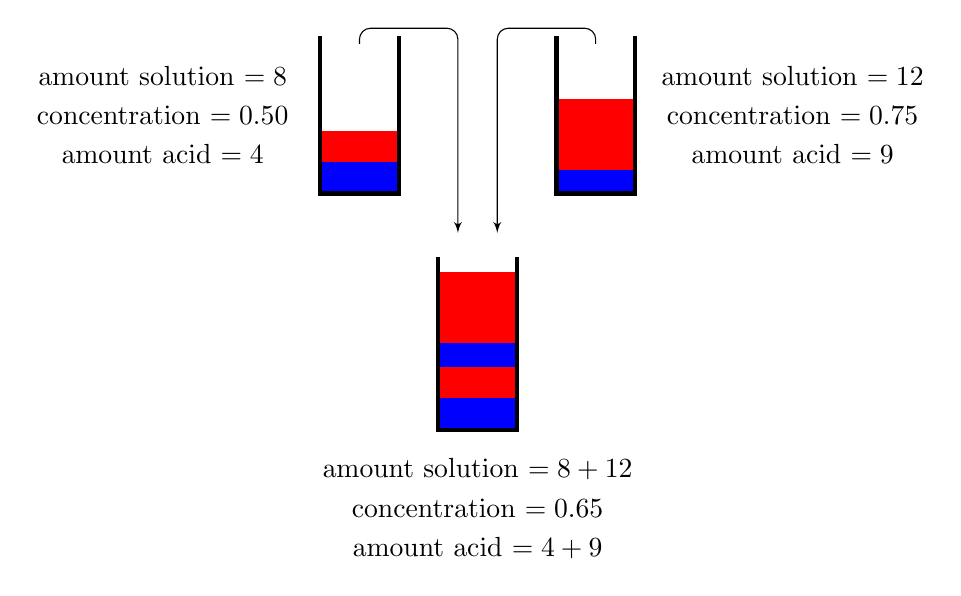
\begin{tikzpicture}
\fill[blue] (-1,0) -- (-2,0) -- (-2,.4) -- (-1,.4) -- cycle;
\fill[red] (-1,.4) -- (-2,.4) -- (-2,.8) -- (-1,.8) -- cycle;
\draw[ultra thick] (-1,2) -- (-1,0) -- (-2,0) -- (-2,2);
%
\fill[blue] (1,0) -- (2,0) -- (2,.3) -- (1,.3) -- cycle;
\fill[red] (1,.3) -- (2,.3) -- (2,1.2) -- (1,1.2) -- cycle;
\draw[ultra thick] (1,2) -- (1,0) -- (2,0) -- (2,2);
%
\fill[blue] (-.5,-3) -- (.5,-3) -- (.5,-2.6) -- (-.5,-2.6) -- cycle;
\fill[red] (-.5,-2.6) -- (.5,-2.6) -- (.5,-2.2) -- (-.5,-2.2) -- cycle;
\fill[blue] (-.5,-2.2) -- (.5,-2.2) -- (.5,-1.9) -- (-.5,-1.9) -- cycle;
\fill[red] (-.5,-1.9) -- (.5,-1.9) -- (.5,-1) -- (-.5,-1) -- cycle;
\draw[ultra thick] (-.5,-0.8) -- (-.5,-3) -- (.5,-3) -- (.5,-0.8);
%
\path[line, rounded corners] (-1.5, 1.9) -- (-1.5,2.1) -- (-0.25,2.1) -- (-0.25,-0.5);
\path[line, rounded corners] (1.5, 1.9) -- (1.5,2.1) -- (0.25,2.1) -- (0.25,-0.5);
%
\node at (-4,1.5) {amount solution $= 8$};
\node at (-4,1.0) {concentration $= 0.50$};
\node at (-4,0.5) {amount acid $= 4$};
%
\node at (4,1.5) {amount solution $= 12$};
\node at (4,1.0) {concentration $= 0.75$};
\node at (4,0.5) {amount acid $= 9$};
%
\node at (0,-3.5) {amount solution $= 8+12$};
\node at (0,-4.0) {concentration $= 0.65$};
\node at (0,-4.5) {amount acid $= 4+9$};
\end{tikzpicture}
\end{center}


%\newpage


\begin{exm}
How many liters of a $20\%$ acid solution should be mixed with $80$ liters of a $61\%$ acid solution to make a $45\%$ acid solution?
\end{exm}
\vskip10pt
\begin{exm}
How many liters of a $20\%$ acid solution and how many liters of a $61\%$ acid solution should be mixed together to make $80$ liters of a $45\%$ acid solution?
\end{exm}
\vskip10pt

%\newpage

\begin{bmethod}{Mixture}{}
Every mixture problem can be rephrased as taking the contents of one beaker and the contents of another beaker and dumping both into a bucket. Since the concentration equation must be applied to each container, for each container, you must keep track of the \underline{amount of solution}, the \underline{concentration of acid}, and the \underline{amount of acid}. Be sure to address the following:
\begin{itemize}
\item Apply the concentration equation to Beaker 1.
\item Apply the concentration equation to Beaker 2.
\item Apply the concentration equation to the final bucket.
\item The amount of solution in the bucket is the sum of the amount of solution in Beaker 1 and the amount of solution in Beaker 2.
\item The amount of acid in the bucket is the sum of the amount of acid in Beaker 1 and the amount of acid in Beaker 2.
\item You will always obtain two expressions for the amount of acid in the bucket, so equate these.
\end{itemize}
\end{bmethod}



Extra practice problems:
\begin{enumerate}

\item
A jar has liquid. Some of the liquid is acid, and some of the liquid is non-acid. If the jar has $8$ liters of liquid and $50\%$ of the jar is acid, how many liters of acid are in the jar?
\item
If a $5$ liter jar is $84\%$ acid, how much of the jar (in liters) is acid?
\item
You have an empty bucket. An $8$ liter jar which is $50\%$ acid is dumped into the bucket. A $5$ liter jar which is $84\%$ acid is also dumped into the bucket.
\begin{enumerate}
\item What is the total volume of liquid in the bucket (in liters)?
\item How many liters of acid are in the bucket?
\item What is the concentration (as a percent) of acid in the bucket?
\end{enumerate}
\item What amount of a 60\% acid solution must be mixed with a 30\% solution to produce $24$ liters of a 50\% solution?
\item
A manufacturer of soft drinks advertises their orange soda as ``naturally flavored,'' although it contains only 5\% orange juice. A new federal regulation stipulates that to be called ``natural,'' a drink must contain at least 10\% fruit juice. How much pure orange juice must this manufacturer add to $500$ gallons of orange soda to conform to the new regulation?
\end{enumerate}



%\newpage

Additional practice problems:
\everymath{\displaystyle}
\begin{exm}{A woman earns 15\% more than her husband. Together they make \$69,875. What is the husband's salary?}
\end{exm}
\begin{exm}{A plumber and his assistant work together. The plumber charges \$45 an hour and his assistant charges \$25 an hour. The plumber works twice as long as his assistant on a job and the final bill for both workers is\$4,025. How long did the plumber and his assistant work?}
\end{exm}
\begin{exm}{A man walking away form a lamppost with a light source 6 meters above the ground. The man is 2 meters tall. How long is the man's shadow when he is 10 meters from the lamppost?}
\end{exm}
\begin{exm}{A pot contains 6 liters f brine at a concentration of 120 g/L. How much water should be boiled off to increase the concentration to 200 g/L?}
\end{exm}
\begin{exm}{ Two cyclists, 90 miles apart, start riding toward each other at the same time. One cycles twice as fast as the other. If they 2 hours later, at what average speed is each cyclist traveling?}
\end{exm}
\begin{exm}{If Ben invests \$4000 at 4\% interest per year, how much additional money must he invest at 5.5\% annual interest to ensure that the interest he receives each year is 4.5\% of the total amount invested?}
\end{exm}


\renewcommand{\booksection}{The $xy$-plane}
\renewcommand{\pageheader}{\booksection }
\section*{\LARGE \pageheader}

\section{$xy$-plane and the Quadrants}
The $xy$-plane can be divided into four quadrants which are described by the behavior of $x$ and $y$. 

				\begin{center}
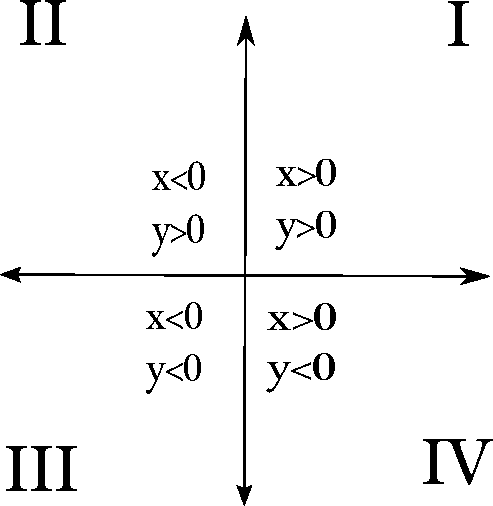
\includegraphics[scale=.85]{quad.pdf}
\end{center}

A point always has an $x$-coordinate and a $y$-coordinate, wrapped inside a set of parentheses.

\begin{bconcept}{}{}
The information about a point can be written by labelling coordinates by the point, or putting tick marks on the axes.
\end{bconcept}
\begin{exm}
Provide both representations of the point $(8,3)$.
\end{exm}

\vskip120pt

In the picture below, the point $(-5,2)$ is part of the graph, but the point $(-5,5)$ is not. The ``unfilled dot'' there is telling is we get all the points between $(-8,2)$ and $(-5,5)$ but not the point $(-8,2)$ itself or the point $(-5,5)$ itself. On the other hand, the graph includes the point $(-1,3)$, even though the point hasn't been drawn in thick.

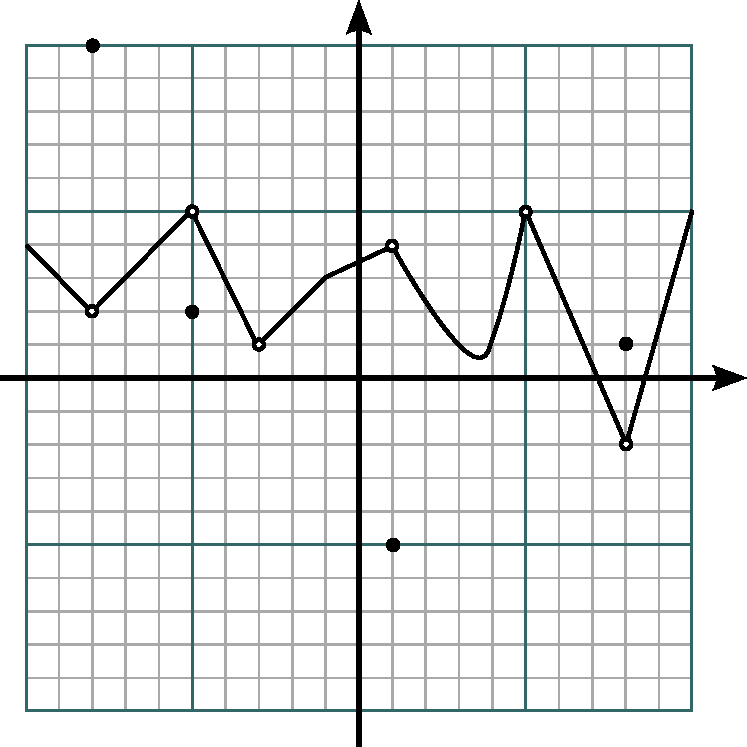
\includegraphics[width=4in]{twosided-limits}


%\newpage



\begin{bformula}{Distance Formula}
Given two points $(x_1, y_1)$ and $(x_2,y_2)$ the {\bf{distance}} between these points is given by $$d=\sqrt{(x_2-x_1)^2+(y_2-y_1)^2}.$$ 
\end{bformula}

This comes from the Pythagorean Theorem which states that a right triangle with sides $a$ and $b$ and hypotenuse $c$ satisfies the equation $$a^2+b^2=c^2,$$ 


\everymath{\displaystyle}
\begin{exm}{Show that $(-6,3),~~(-1, 5)$ and $(3,-5)$ are vertices of a right triangle. Then, find the area of that triangle.}
\end{exm}\vskip10pt

\begin{exm}{Find $x$ so that the distance between the two points, $(x,3)$ and $(4,5)$ is 5.}
\end{exm}\vskip10pt

%\newpage
\begin{bformula}{Midpoint Formula}{}
Given two points $(x_1, y_1)$ and $(x_2,y_2)$ the {\bf{midpoint}} between these points is given by $$\left(\frac{x_1+x_2}{2}, \frac{y_1+y_2}{2}\right).$$ Note that this is a point.
\end{bformula}



\everymath{\displaystyle}
\begin{exm}{Given points $A(5,-8)$ and $B(-6, 2)$, find the point on the line segment $AB$ that is $\frac{3}{4}$ of the way from $A$ to $B$.}
\end{exm}\vskip10pt

\begin{exm}{Find the point on the line $y=x$ that is equidistant from $(-2,4)$ and $(4,5)$.}
\end{exm}\vskip10pt





%\newpage
\renewcommand{\booksection}{Graphs of equations}
\renewcommand{\pageheader}{\booksection }
\section*{\LARGE \pageheader}

This section focuses on equations in $x$ and $y$.
\begin{exm}
$x^3+xy+6=x+xy^2$ is an equation in $x$ and $y$
\end{exm}
Every equation in $x$ and $y$ can be graphed on the $xy$-plane.
\begin{bconcept}{How is an equation in $x$ and $y$ related to its graph?}{}
The point $(x,y)$ is part of the graph if and only if $(x,y)$ satisfies the equation.
\end{bconcept}
\begin{exm}
Is the point $(2,3)$ part of the graph of $x^3+xy+6=x+xy^2$?
\end{exm}
\vskip10pt
\begin{exm}
Is the point $(2,1)$ part of the graph of $x^3+xy+6=x+xy^2$?
\end{exm}
\vskip10pt
\begin{exm}
Is the point $(1,4)$ part of the graph of $x^2+2y=20-4x-y^2$?
\end{exm}
\vskip10pt
\begin{exm}
Is the point $(1,3)$ part of the graph of $x^2+2y=20-4x-y^2$?
\end{exm}
\vskip10pt

%\newpage

\qrcode{https://www.desmos.com/calculator/b5c6wq2rtp}
\hskip10pt
\url{https://www.desmos.com/calculator/b5c6wq2rtp}

\begin{exm}
Find three points on the graph of $x=y^2-5$
\end{exm}
\vskip10pt
\begin{exm}
Find three points on the graph of $2y=x^3$
\end{exm}
\vskip10pt


%\newpage
\renewcommand{\booksection}{Graphs of lines}
\renewcommand{\pageheader}{\booksection }
\section*{\LARGE \pageheader}

%
%\begin{concepts}
% \item  Slopes of lines
%	\item Slope intercept equation
%	\item Point slope equation 
%\item Standard equation
%
%\end{concepts}
%



\section{Lines}

In order to find an equation of a line, you need are 2 points or a point and a slope. If you are working on a problem and it asks you to find an equation of a line, you need to ask yourself if you already have 2 points or if you have a point and a slope. This will determine which strategy you should use to answer the problem. 

\section{Slopes of Lines}
In order to find the slope of a line, you will need only two points, generically labeled $(x_1,y_1)$ and $(x_2,y_2)$. Once you have these two points, the slope is given by a formula:
\begin{bdefinition}{Slope}{slope}
$$m=\frac{y_2-y_1}{x_2-x_1} = \frac{\text{rise}}{\text{run}} = \frac{\text{change in $y$}}{\text{change in $x$}} = \frac{\triangle y}{\triangle x}$$
\end{bdefinition}
The phrase ``rise over run'' is meant to help so that we don't accidentally put $x$-values in the numerator. The word ``rise'' lets you know we are talking about the change in height, and the height is given by the $y$-value. Slope is ``rise over run'' not ``run over rise''
\begin{bwarning}{Incorrect slope}{}
$$m \not= \frac{x_2-x_1}{y_2-y_1}$$
\end{bwarning}

\begin{center}
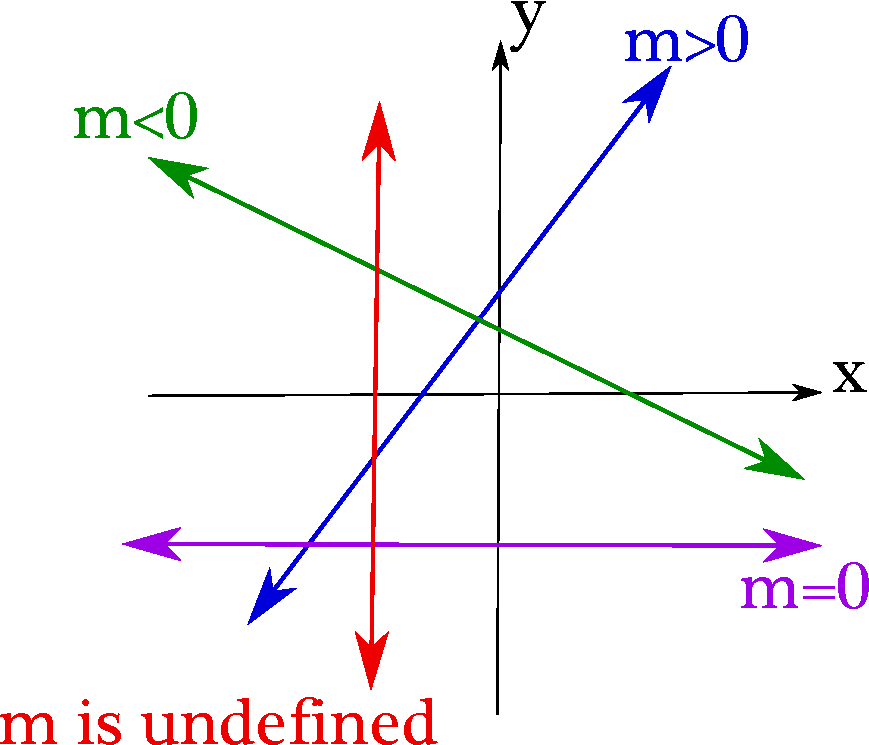
\includegraphics[scale=.4]{slope1.pdf}
\end{center}

\section{Types of Equations}
There are several types of equations of lines and ALL of them are okay to use. (However, sometimes directions to homework problems will specifically ask for one equation or another as an answer. Or, it could be that it makes sense to use one equation over another.)


\begin{bdefinition}{Point-Slope form of a line}{pointslope}
 $$y-y_1=m(x-x_1)$$
 where $m$ is the slope and $(x_1,y_1)$ is {\it any} point on the line.
\end{bdefinition}
\begin{exm}
$y-2=\frac34(x-5)$ describes the line of slope $\frac34$ going through the point $(5,2)$.
\end{exm}

\begin{bdefinition}{Slope-Intercept form of a line}{slopeintercept}
$$y=mx+b$$
where $m$ is the slope and $b$ is the $y$-intercept
\end{bdefinition}
\begin{exm}
$y=\frac67x+8$ describes the line of slope $\frac67$ with $y$-intercept $8$.
\end{exm}
\begin{bwarning}{}{mx-not-slope}
Note that $m$ is the slope in $y=mx+b$, but $mx$ is not the slope.
\end{bwarning}
\begin{exm}
Earlier, we saw that $y=\frac67x+8$ describes the line of slope $\frac67$, but it would be incorrect to report the slope as $\frac67x$. In the format $y=mx+b$, it is the content {\bf before} the $x$ that is the slope, but without including $x$ itself. 
\end{exm}



%\newpage


\everymath{\displaystyle}
\begin{exm}{}
Find the line that passes through the points $(-2,4)$ and $(9,2)$. 
\end{exm}\vskip10pt


\begin{exm}{}
Find the line that passes through the point $(1,3)$ with slope $-\frac{1}{4}$
\end{exm}\vskip10pt

%\newpage
\begin{exm}{}
Find the line that passes through the point $(2,5)$ with $x$-intercept 4.
\end{exm}\vskip10pt

\begin{exm}{}
Find the slope of the line given by $3x+4y=9$. 
\end{exm}\vskip10pt

%\newpage
\begin{exm}{}
Does the line given by $3x+4y=9$ pass through the point $(1,1)$? Explain your reasoning.
\end{exm}\vskip10pt

\begin{exm}{}
Does the line given by $3x+4y=9$ pass through the point $(3,0)$? Explain your reasoning.
\end{exm}\vskip10pt

%\newpage
\begin{exm}{}
In finding the line that passes through the points $(-2,4)$ and $(9,2)$, does it matter which point is $(x_1,y_1)$ and which point is $(x_2,y_2)$? Explain.
\end{exm}\vskip10pt

%\newpage

\begin{bfact}{Parallel lines}{}
Two lines are parallel if they have the same slope. 
\end{bfact}
\qrcode{https://www.desmos.com/calculator/taifhuenas}
\hskip10pt
\url{https://www.desmos.com/calculator/taifhuenas}

\begin{bfact}{Perpendicular lines}{}
 Two lines are perpendicular if their slopes are negative reciprocals. In other words, if line 1 has slope $m_1$ and line 2 has slope $m_2$, then $$m_1=\frac{-1}{m_2}~~~~ \mbox{or}~~~~ m_1\cdot m_2=-1$$ 
\end{bfact}
\qrcode{https://www.desmos.com/calculator/i6svrb0s6u}
\hskip10pt
\url{https://www.desmos.com/calculator/i6svrb0s6u}

%\newpage

\everymath{\displaystyle}
\begin{exm}{}Sketch a graph of the line that passes through the points $(-2,4)$ and $(9,2)$.
\end{exm}\vskip10pt

\begin{exm}{}Sketch a graph of the line line that passes through the point $(1,3)$ with slope $\frac{-1}{4}$. 
\end{exm}\vskip10pt

%\newpage
\begin{exm}{}Sketch a graph of the line that passes through the point $(2,5)$ with $x$-intercept 4.
\end{exm}\vskip10pt

\begin{exm}{}Find an equation of the line which is parallel to $3x+2y=1$ that passes through the point $(1,1)$. Then, sketch a graph of both lines.
\end{exm}\vskip10pt

%\newpage
\begin{exm}{}Find an equation of the line that is perpendicular to $y=3x+1$ that passes through the point $(-2,1)$. Then, sketch a graph of both lines.
\end{exm}\vskip10pt

\begin{exm}{}Sketch the line given by $y=2x+1$.
\end{exm}\vskip10pt

%\newpage
\begin{exm}{}Sketch the line given by $y-3=2(x+1)$.
\end{exm}\vskip10pt

\begin{exm}{}Sketch the line given by $2x-3y=1$
\end{exm}\vskip10pt

%\newpage

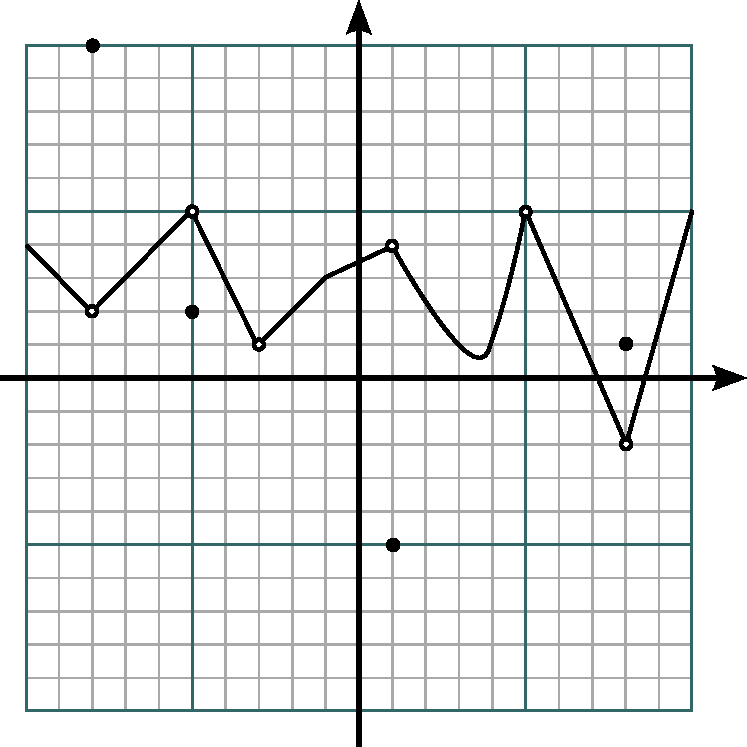
\includegraphics[width=4in]{twosided-limits}

\begin{exm}\label{interpolation}
In the graph above, find the $y$-value of the point in the graph when the $x$-value is $6$.
\end{exm}


%\newpage
\renewcommand{\booksection}{Applications of geometry in the $xy$-plane}
\renewcommand{\pageheader}{\booksection }
\section*{\LARGE \pageheader}
%\begin{concepts}
%\item applications
%\end{concepts}

\begin{exm}
The two lines $y=\frac38x+17$ and $y=-\frac14x+42$ intersect\footnote{This is a typical {\bf business} problem in the area of supply and demand. In business, supply always has positive slope and demand has negative slope. So, if $y=\frac38x+17$ represents supply and $y=-\frac14x+42$ represents demand, then the intersection point that this question asked for is called the {\bf equilibrium}.} at a point. Find the point.
\end{exm}
\vskip10pt

\begin{exm}
Find the area of the region below $y=2x$, above the $x$-axis, and between the lines $x=7$ and $x=10$. (There are at least two ways to do this.)
\end{exm}
\vskip10pt

%\newpage

% https://www.desmos.com/calculator/yocgrxjivw
\begin{exm}
In the image below, the blue line has equation $y=\frac23x+3$ and the red line has equation $y=-\frac16x+8$. The purple line is a horizontal line drawn by the intersection of the red and blue lines. Find the area of the shaded region\footnote{In {\bf economics}, if the blue line represents supply and the red line represents demand, then the area requested represent {\bf producer surplus}.}. 
\vskip1pt
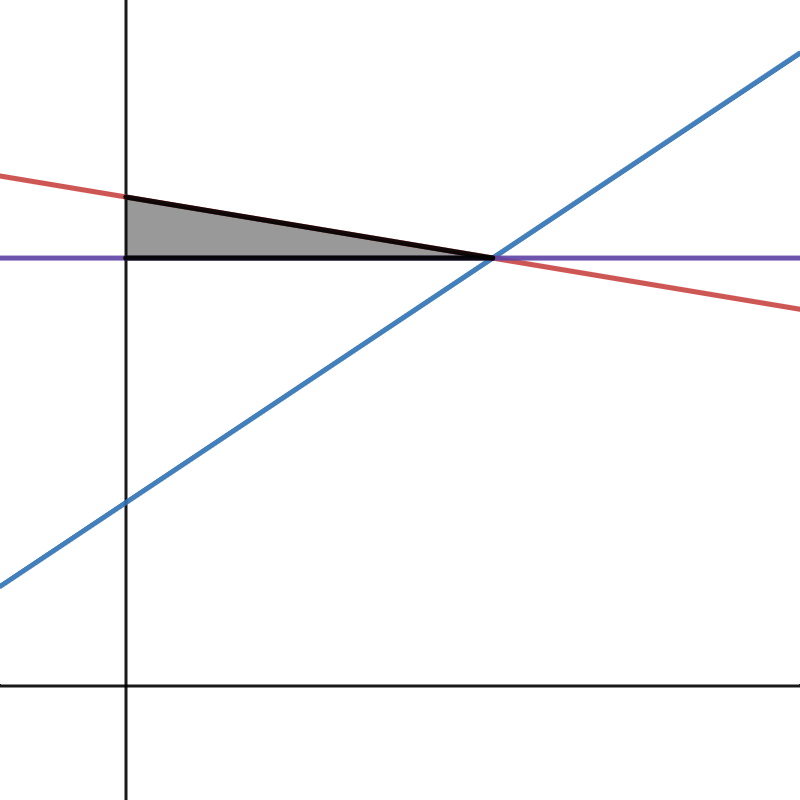
\includegraphics[width=3.0in]{psurplus}
\end{exm}

%\newpage

% https://www.desmos.com/calculator/yocgrxjivw
\begin{exm}
In the image below, the blue line has equation $y=mx+b$ and the red line has equation $y=nx+c$. Find the area\footnote{In {\bf economics}, if the blue line represents supply and the red line represents demand, then the area requested represent {\bf producer surplus}.} of the shaded region in terms of $m$, $b$, $n$, and $c$.
\vskip1pt
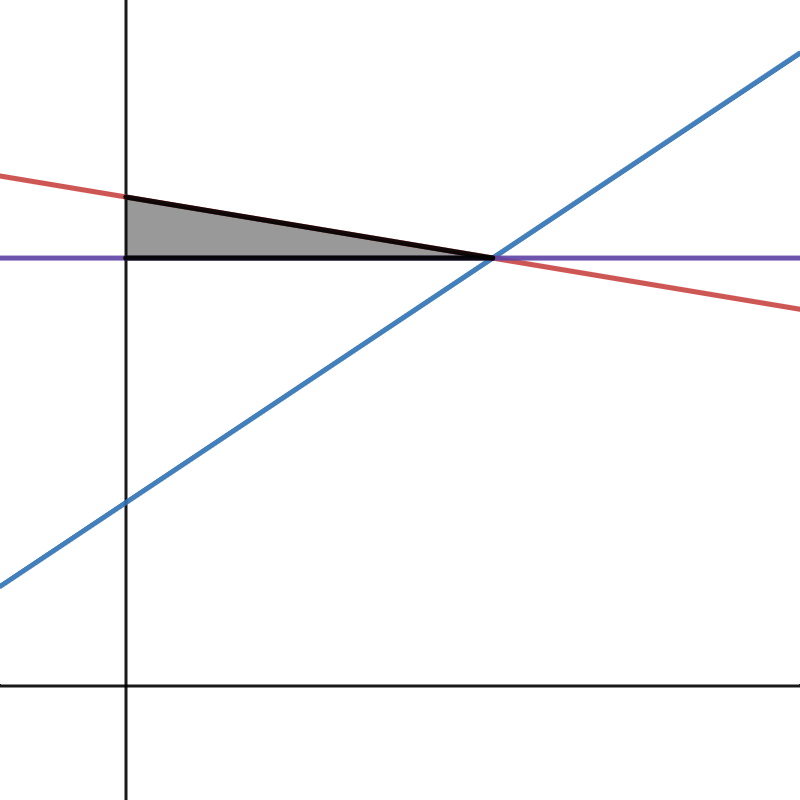
\includegraphics[width=3.0in]{psurplus}
\end{exm}

%\newpage

% https://www.desmos.com/calculator/bxdgvvqkgm
\begin{exm}
In the image below, the blue line has equation $y=10-x$ and the red line has equation $y=2x+1$. The purple horizontal line is $y=9$, and the vertical purple lines are created by the intersection of the horizontal line with the red and blue lines. Find the area of the shaded region. The purple line is a horizontal line drawn by the intersection of the red and blue lines. Find the area\footnote{In {\bf economics}, this area represents {\bf government expenditures}.} of the shaded region. 
\vskip1pt
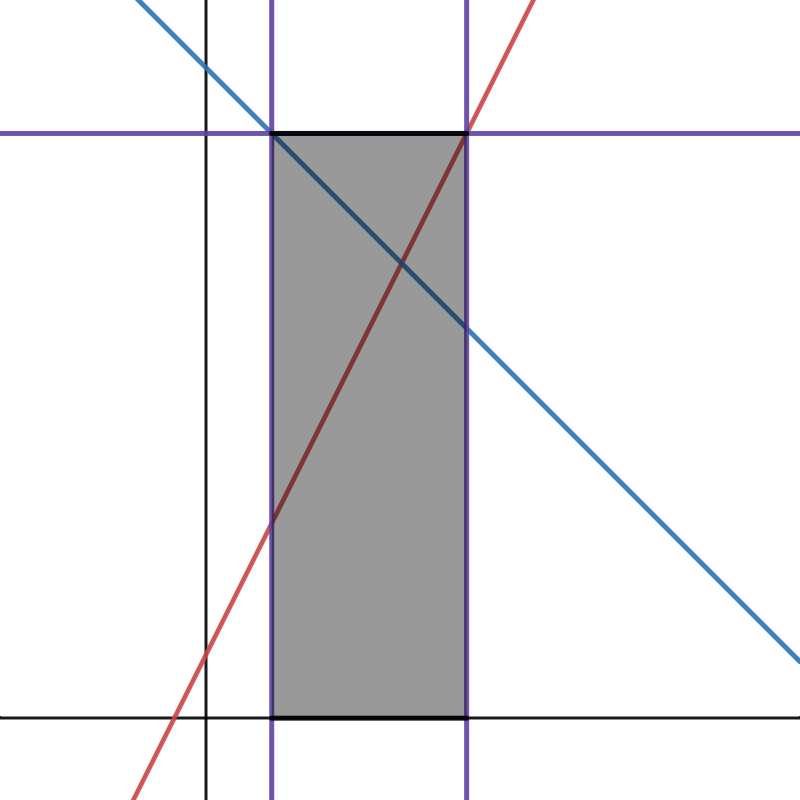
\includegraphics[width=3.0in]{govexp}
\end{exm}


%\newpage
\renewcommand{\booksection}{Graph interpretation}
\renewcommand{\pageheader}{\booksection }
\section*{\LARGE \pageheader}
%\begin{concepts}
%\item Interpret graphs
%\item Describe the growth/shrinkage of quantities
%\end{concepts}

An all areas where math gets used (economics, biology, chemistry, physics, sociology, weather forecasting, etc.) graphs are presented to show how one quantity relates to another. One quantity is labeled on the $x$-axis, and one on the $y$-axis.

Examine the following graph from NASA, originally found at 
\vskip1pt
\qrcode{https://earthobservatory.nasa.gov/features/GlobalWarming/page2.php}
\vskip1pt
\url{earthobservatory.nasa.gov/features/GlobalWarming/page2.php}

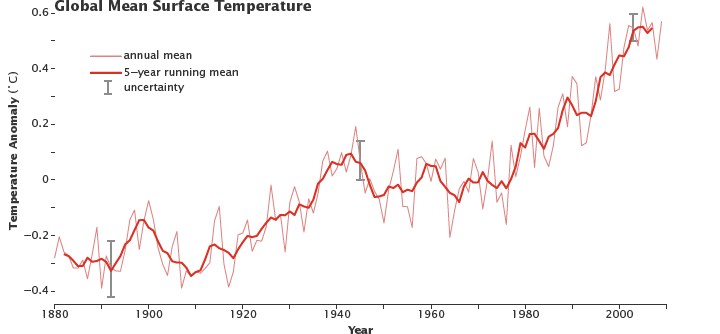
\includegraphics[width=\textwidth]{global-temperature}

The picture above has the complication that two graphs are presented together. Let's look at the thicker graph. What we are seeing is that the further into the future we look (the year, which is the $x$-value, increases), it gets hotter. (I say ``hotter'' because the $y$-axis represents temperature, and bigger temperature values means hotter rather than colder.)

Because people talk about global warming, it is too easy to come up with the correct thing to say: it is easy to say what the graph is saying without actually looking at the graph. However, in future classes where you will look at an interpret graphs, you will probably not always get to rely on your intuition.

%\newpage

Here is an actual example from {\bf economics}, slightly simplified.

\begin{exm}
Interpret the graph below
\end{exm}
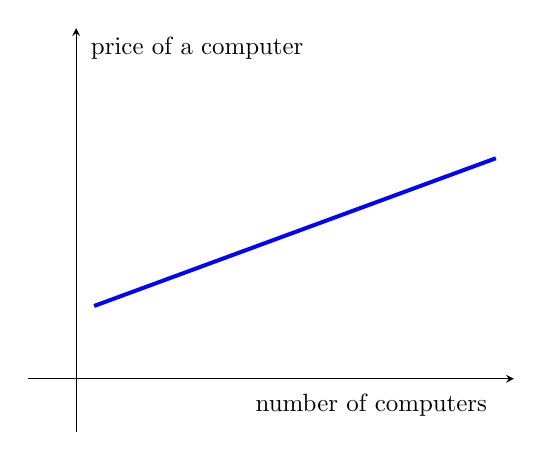
\begin{tikzpicture}[scale=0.9]
\begin{axis}[%grid=both,
 axis lines=middle,
 ticklabel style={fill=white},
 xmin=-.8,xmax=7.3,
 ymin=-.8,ymax=5.3,
 xtick={0}, ytick={0},
% xtick={-4,-2,2,4},     %<--
% ytick={-4,-2,2,4},          %<--
% minor tick = {-5,-3,...,5}, %<--
 xlabel=\(\),ylabel=\(\),
 samples=10]
\addplot[ultra thick, blue, domain=.3:7,-] {x/3+1};
\node at (axis cs: 7,-.4)[anchor=east] {number of computers};
\node at (axis cs: .1,5)[anchor=west] {price of a computer};
\end{axis}
\end{tikzpicture}
\vskip4pt
{\bf Answer:} If there are more computers, then each computer gets \underline{\phantom{................................}}

\begin{exm}
Interpret the graph below
\end{exm}
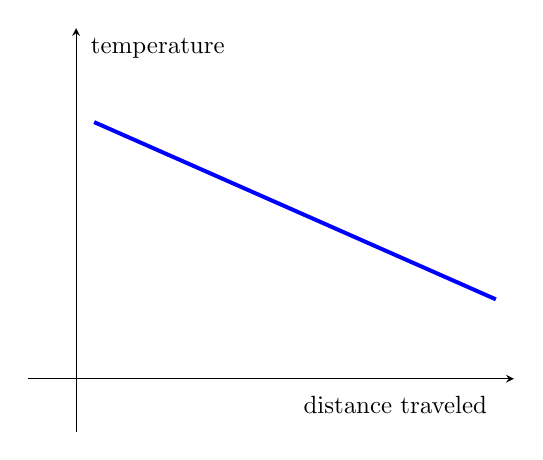
\begin{tikzpicture}[scale=0.9]
\begin{axis}[%grid=both,
 axis lines=middle,
 ticklabel style={fill=white},
 xmin=-.8,xmax=7.3,
 ymin=-.8,ymax=5.3,
 xtick={0}, ytick={0},
% xtick={-4,-2,2,4},     %<--
% ytick={-4,-2,2,4},          %<--
% minor tick = {-5,-3,...,5}, %<--
 xlabel=\(\),ylabel=\(\),
 samples=10]
\addplot[ultra thick, blue, domain=.3:7,-] {-x/2.5+4};
\node at (axis cs: 7,-.4)[anchor=east] {distance traveled};
\node at (axis cs: .1,5)[anchor=west] {temperature};
\end{axis}
\end{tikzpicture}
\vskip4pt
The longer the distance traveled,  the \underline{\phantom{................................}} it gets

\begin{exm}
Interpret the graph below
\end{exm}
\begin{tikzpicture}[scale=0.9]
\begin{axis}[%grid=both,
 axis lines=middle,
 ticklabel style={fill=white},
 xmin=-.8,xmax=7.3,
 ymin=-.8,ymax=5.3,
 xtick={0}, ytick={0},
% xtick={-4,-2,2,4},     %<--
% ytick={-4,-2,2,4},          %<--
% minor tick = {-5,-3,...,5}, %<--
 xlabel=\(\),ylabel=\(\),
 samples=10]
\addplot[ultra thick, blue, domain=.3:7,-] {-x/3+4.5};
\node at (axis cs: 7,-.4)[anchor=east] {number of dolls};
\node at (axis cs: .1,5)[anchor=west] {price};
\end{axis}
\end{tikzpicture}
\vskip4pt
The more dolls there are, the \underline{\phantom{................................}} each doll is

\begin{exm}
Interpret the graph below
\end{exm}
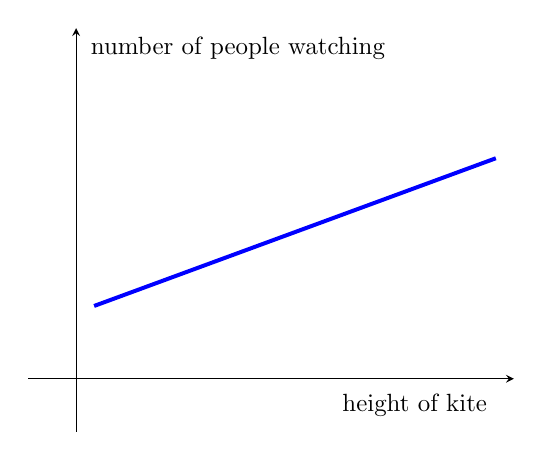
\begin{tikzpicture}[scale=0.9]
\begin{axis}[%grid=both,
 axis lines=middle,
 ticklabel style={fill=white},
 xmin=-.8,xmax=7.3,
 ymin=-.8,ymax=5.3,
 xtick={0}, ytick={0},
% xtick={-4,-2,2,4},     %<--
% ytick={-4,-2,2,4},          %<--
% minor tick = {-5,-3,...,5}, %<--
 xlabel=\(\),ylabel=\(\),
 samples=10]
\addplot[ultra thick, blue, domain=.3:7,-] {x/3+1};
\node at (axis cs: 7,-.4)[anchor=east] {height of kite};
\node at (axis cs: .1,5)[anchor=west] {number of people watching};
\end{axis}
\end{tikzpicture}
\vskip4pt
The higher a kite is, \underline{\phantom{................................}}

\begin{exm}
Interpret the graph below
\end{exm}
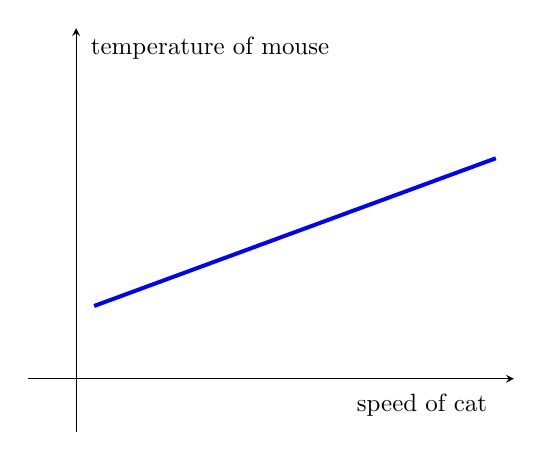
\begin{tikzpicture}[scale=0.9]
\begin{axis}[%grid=both,
 axis lines=middle,
 ticklabel style={fill=white},
 xmin=-.8,xmax=7.3,
 ymin=-.8,ymax=5.3,
 xtick={0}, ytick={0},
% xtick={-4,-2,2,4},     %<--
% ytick={-4,-2,2,4},          %<--
% minor tick = {-5,-3,...,5}, %<--
 xlabel=\(\),ylabel=\(\),
 samples=10]
\addplot[ultra thick, blue, domain=.3:7,-] {x/3+1};
\node at (axis cs: 7,-.4)[anchor=east] {speed of cat};
\node at (axis cs: .1,5)[anchor=west] {temperature of mouse};
\end{axis}
\end{tikzpicture}
\vskip4pt
As the cat moves faster, \underline{\phantom{................................}}

\begin{exm}
Interpret the graph below
\end{exm}
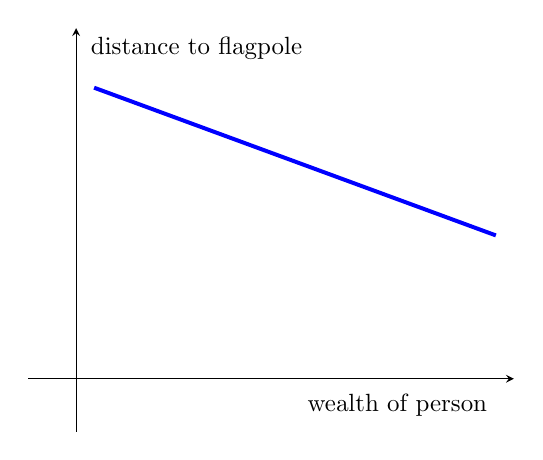
\begin{tikzpicture}[scale=0.9]
\begin{axis}[%grid=both,
 axis lines=middle,
 ticklabel style={fill=white},
 xmin=-.8,xmax=7.3,
 ymin=-.8,ymax=5.3,
 xtick={0}, ytick={0},
% xtick={-4,-2,2,4},     %<--
% ytick={-4,-2,2,4},          %<--
% minor tick = {-5,-3,...,5}, %<--
 xlabel=\(\),ylabel=\(\),
 samples=10]
\addplot[ultra thick, blue, domain=.3:7,-] {-x/3+4.5};
\node at (axis cs: 7,-.4)[anchor=east] {wealth of person};
\node at (axis cs: .1,5)[anchor=west] {distance to flagpole};
\end{axis}
\end{tikzpicture}
\vskip4pt




%\newpage
\renewcommand{\booksection}{Quadratic Equations}
\renewcommand{\pageheader}{\booksection }
\section*{\LARGE \pageheader}

%A \underline{quadratic equation} is an equation of the form: $$ax^2+bx+c=0,$$ where $a,b,c$ are real numbers and $a\neq0$.  A quadratic is a polynomial of degree $2$. 

Our goal is to solve equations such as $5x^2+8x-1=6$


%There are many ways to solve a quadratic such as factoring, quadratic formula, completing the square. Not all of them will work the same way, so you must choose carefully.
%
% To solve an equation means to find numbers that can be substituted into the equation for the variables so that the equation remains true. Here are some examples: 
%\begin{itemize}
%    \item $-3$ is a solution to $x+3=0$ since $-3+3=0$
%    \item $3$ is not a solution to $x+3=0$ since $3+3\neq 0$
%    \item $2$ is a solution to the equation $x^2=4$ since $2^2=4$
%    \item $1$ is not a solution to $x^2+1=0$ since $1^1+1\neq 0$
%\end{itemize}
%
%
%\section{Factoring by Grouping}
%Let's look at an example in which we want to find the solutions to $x$: $$x^2-x-6=0$$.
%We need to find two numbers that sum to $b$ and multiply to give $c$ in the general expression $$x^2+bx+c=0.$$ For this example, we want 2 numbers that sum to -1 and multiply to give -6. These numbers are -3 and 2. 
% 
% Next, we rewrite the quadratic using these 2 numbers: $$x^2-x-6=x^2+2x+ -3x+(2\cdot -3)$$
%and factor by grouping: $$x^2+2x+ -3x+(2\cdot -3)=x(x+2)+-3(x+2) =(x+2)(x-3)$$
%
%Now, since the product $(x+2)(x-3)$ equals 0, we set each term equal to zero and solve for $x$: 
%$$x-3=0~~~~~~~~~~~~x+2=0\Longrightarrow x=3~~~~~~~~~~~x=-2$$
%
% When solving an equation, you should always check your work: $$(3)^2-(3)-6=0~~~~~~~~~~~~~~~~~~~~~~~~(-2)^2-(-2)-6=0.$$
%
%\everymath{\displaystyle}
%\begin{exm}{}Solve $x^2-9=0$
%\end{exm}\vskip10pt
%
%\everymath{\displaystyle}
%\begin{exm}{}Solve $x^2+13=30$
%\end{exm}\vskip10pt
%
%%\newpage
%\everymath{\displaystyle}
%\begin{exm}{}Solve $6x^2=1-x$
%\end{exm}\vskip10pt
%
%\everymath{\displaystyle}
%\begin{exm}{}Try to solve $x^2+3x-5=0$. What can you conclude?
%\end{exm}\vskip10pt

\begin{bmethod}{Zero Product Property}{}
If $ab=0$ then $a=0$ or $b=0$
\end{bmethod}
\begin{exm}
Justify the Zero Product Property based on the geometric interpretation of multiplication.
\end{exm}
\vskip10pt
\begin{exm}
If $ab = 14$, can we conclude $a=14$ or $b=14$?
\end{exm}
\vskip10pt
\begin{exm}
Solve $x^2-8x+15=0$
\end{exm}
\vskip10pt
\begin{exm}
Solve $x^2-3x=0$
\end{exm}
\vskip10pt

%\newpage

\begin{exm}
Solve $x^2-x=6$
\end{exm}
\vskip10pt
\begin{bmethod}{Zero Product Property, extended version}{}
If $abc=0$ then $a=0$ or $b=0$ or $c=0$
\end{bmethod}
\begin{exm}
Solve $x^3+12x=7x^2$
\end{exm}
\vskip10pt

%\newpage

\begin{bmethod}{}{}
\begin{enumerate}
\item
Take a given equation and add/subtract on both sides to get one side to be $0$.
\item If the other side factors, then apply the Zero Product Property. (If the other side does not factor, then try something else, since we're stuck.)
\end{enumerate}
\end{bmethod}

\begin{exmref}\label{x249}
Solve $x^2-49=0$
\end{exmref}
\vskip10pt
\begin{exm}
Solve $x^2-10x+21=0$
\end{exm}
\vskip10pt
\begin{exm}
Solve $x^2+16=8x$
\end{exm}
\vskip10pt
\begin{exmref}\label{x2144}
Solve $x^2=144$
\end{exmref}
\vskip10pt

%\newpage

\begin{bmethod}{Square rooting both sides of an equation}{}
Given an equation, make a copy of the equation one line below, and square root both sides, placing a $\pm$ sign on one side.
\end{bmethod}
Note that simplifying a square root {\bf expression} (See Concept\ref{concept:radical-mean}) does not involve $\pm$, but taking the action of square rooting both sides of an {\bf equation} introduces $\pm$

\begin{bmethod}{Quadratic equations without linear terms}{}
To solve a quadratic equation with no linear term,
\begin{enumerate}
\item Add/subtract to get the quadratic term on one side and the constant term on the other side.
\item Square root both sides.
\end{enumerate}
\end{bmethod}

Though the first two questions questions on this page were on the previous page (Example \ref{x249} and Example \ref{x2144}), solve using the method introduced on this page.
\begin{exm}
Solve $x^2-49=0$
\end{exm}
\vskip10pt

\begin{exm}
Solve $x^2=144$
\end{exm}
\vskip10pt

\begin{exm}
Solve $(x-6)^2=19$
\end{exm}
\vskip10pt

%\newpage

\begin{exm}
Solve $(x+3)^2=5$
\end{exm}
\vskip10pt

\begin{exm}
Geometrically justify $(a+b)(c+d)=ac+ad+bc+bd$
\end{exm}
\vskip10pt

\begin{exm}
Draw $x \cdot x$, also known as $x^2$
\end{exm}
\vskip10pt

%\newpage

\begin{exm}
Draw $(x+y)(x+y)$, and show the contribution of each term in the expanded form.
\end{exm}
\vskip10pt

\begin{exm}
Draw $(x+5)(x+5)$, and show the contribution of each term in the expanded form.
\end{exm}
\vskip10pt

%\newpage


\begin{tikzpicture}
\draw (0,0) -- (3,0) -- (3,3) -- (0,3) -- cycle;
\draw (3,0) -- (4,0) -- (4,3) -- (3,3);
\draw (0,0) -- (0,-1) -- (3,-1) -- (3,0);
\draw (3,-1) -- (4,-1) -- (4,0); % new
%
\node at (-.3,1.5) {$x$};
\node at (-.3,-.5) {$7$};
\node at (1.5,3.3) {$x$};
\node at (3.5,3.6) {$7$};
%
\node at (1.5,1.5) {$x^2$};
\node at (3.5,1.5) {$7x$};
\node at (1.5,-.5) {$7x$};
\node at (3.5,-.5) {$49$}; % new
\end{tikzpicture}

In the picture above, we see\\ $(x+7)^2 = (x+7)(x+7) = x^2 + 7x + 7x + 49 = x^2+14x + 49$
\begin{bconcept}{}{}
\begin{itemize}
\item The length of the second stick is $7$
\item The linear coefficient is $14$, double the length of the second stick.
\item The constant is $49$, the square of the length of the second stick.
\end{itemize}
\end{bconcept}

\vskip40pt
\begin{exm}
Draw $x^2+20x+100$, but first rewrite the linear term.
\end{exm}

%\newpage


\begin{tikzpicture}
\draw (0,0) -- (3,0) -- (3,3) -- (0,3) -- cycle;
\draw (3,0) -- (4,0) -- (4,3) -- (3,3);
\draw (0,0) -- (0,-1) -- (3,-1) -- (3,0);
%
\node at (-.3,1.5) {$x$};
\node at (-.3,-.5) {$3$};
\node at (1.5,3.3) {$x$};
\node at (3.5,3.6) {$3$};
%
\node at (1.5,1.5) {$x^2$};
\node at (3.5,1.5) {$3x$};
\node at (1.5,-.5) {$3x$};
\end{tikzpicture}

\begin{exm}
In the picture above, what is the missing amount that if added would complete the square?
\end{exm}

%\newpage

If you see $x^2+6x$, think of this as $x^2+3x+3x$. Adding $9$ to $x^2+3x+3x$ would make a square.
\vskip10pt

\begin{exm}
What should be added to $x^2+16x$ to complete the square? Draw a picture of $x^2+16x$ and draw a picture of the completed square after adding.
\end{exm}
\vskip10pt

\begin{exm}
What should be added to $x^2+12x$ to complete the square? Draw the before and after pictures.
\end{exm}
\vskip10pt

%\newpage

\begin{exm}
Solve $x^2+12x=5$
\end{exm}
\vskip10pt

\begin{exm}
Solve $x^2+6x=10$
\end{exm}
\vskip10pt

\begin{exm}
Solve $x^2+22x=-20$
\end{exm}
\vskip10pt

%\newpage

\fbox{Linear coefficient} divide by $2$ $\rightarrow$ \fbox{Second stick} square $\rightarrow$ \fbox{number to add}

\begin{exm}
Solve $x^2+22x=-100$
\end{exm}
\vskip10pt

\begin{exm}
Solve $x^2+14x+3=5$
\end{exm}
\vskip10pt

%\newpage

\begin{exm}
Solve $x^2-10x-4=2$
\end{exm}
\vskip10pt

\begin{exm}
Solve $x^2-6x+1=21$
\end{exm}
\vskip10pt

%\newpage


\begin{exm}
Solve $x^2+5x=7$
\end{exm}
\vskip10pt
\vskip10pt

\begin{exm}
Solve $3x^2+5x=6$
\end{exm}
\vskip10pt
\vskip10pt
\vskip10pt

%\newpage

The last example showed us:
\begin{bmethod}{}{}
Before computing second stick, etc. if the coefficient of $x^2$ is not $1$, then divide both sides by the number that is in front of $x^2$ first.
\end{bmethod}

\begin{exm}
Solve $x^2+2x=15$ two different ways.
\end{exm}

%\newpage
\begin{exm}
Complete the square to solve for $x$ in $ax^2+bx+c=0$
\end{exm}


%\newpage

.

%\newpage

.
\vskip10pt

\fbox{
\begin{minipage}[ht]{6.5in}
\vskip4pt
\begin{itemize}
\item The linear coefficient is $\dfrac{b}{a}$, not $\dfrac{b}{a}x$. Do not include the $x$.
\item Since the linear coefficient is $\dfrac{b}{a}$, the length of the second stick is $\dfrac{b}{a} \div 2 = \dfrac{b}{a} \div \dfrac21 = \dfrac{b}{a} \cdot \dfrac12 = \dfrac{b}{2a}$
\item Since the second stick is $\dfrac{b}{2a}$, the constant to add to both sides is $\left(\dfrac{b}{2a}\right)^2 = \dfrac{b^2}{(2a)^2} = \dfrac{b^2}{2^2a^2} = \dfrac{b^2}{4a^2}$
\end{itemize}

\begin{center}
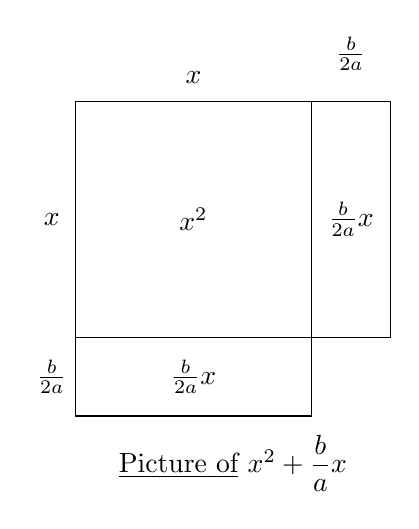
\begin{tikzpicture}
\node at (2,-1.6) {\underline{Picture of} $x^2+\dfrac{b}{a}x$};
\draw (0,0) -- (3,0) -- (3,3) -- (0,3) -- cycle;
\draw (3,0) -- (4,0) -- (4,3) -- (3,3);
\draw (0,0) -- (0,-1) -- (3,-1) -- (3,0);
%
\node at (-.3,1.5) {$x$};
\node at (-.3,-.5) {$\frac{b}{2a}$};
\node at (1.5,3.3) {$x$};
\node at (3.5,3.6) {$\frac{b}{2a}$};
%
\node at (1.5,1.5) {$x^2$};
\node at (3.5,1.5) {$\frac{b}{2a}x$};
\node at (1.5,-.5) {$\frac{b}{2a}x$};
\end{tikzpicture}
\hskip60pt
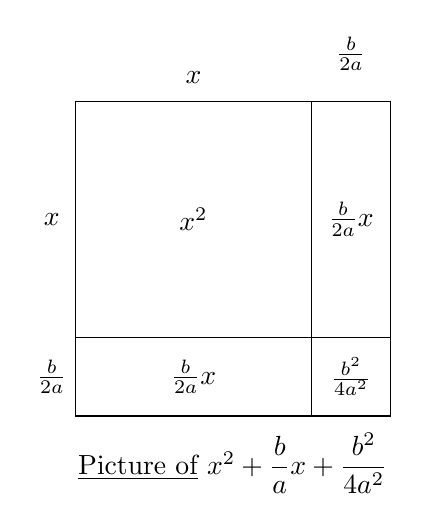
\begin{tikzpicture}
\node at (2,-1.6) {\underline{Picture of} $x^2+\dfrac{b}{a}x+\dfrac{b^2}{4a^2}$};
\draw (0,0) -- (3,0) -- (3,3) -- (0,3) -- cycle;
\draw (3,0) -- (4,0) -- (4,3) -- (3,3);
\draw (0,0) -- (0,-1) -- (3,-1) -- (3,0);
\draw (3,-1) -- (4,-1) -- (4,0); % new
%
\node at (-.3,1.5) {$x$};
\node at (-.3,-.5) {$\frac{b}{2a}$};
\node at (1.5,3.3) {$x$};
\node at (3.5,3.6) {$\frac{b}{2a}$};
%
\node at (1.5,1.5) {$x^2$};
\node at (3.5,1.5) {$\frac{b}{2a}x$};
\node at (1.5,-.5) {$\frac{b}{2a}x$};
\node at (3.5,-.5) {$\frac{b^2}{4a^2}$}; % new
\end{tikzpicture}
\end{center}
\end{minipage}}

%\newpage

\begin{bformula}{Quadratic Formula}{qf}
Given any quadratic equation $ax^2+bx+c=0$,\\ the two solutions of this equation are $$x=\frac{-b\pm\sqrt{b^2-4ac}}{2a}$$ 
\end{bformula}
We just obtained this formula (and you can see the work in the appendix on page~\pageref{derive-qf}).

The expression \fbox{$b^2-4ac$} found inside the square root is called the {\it discriminant} and can be used to tell you the \textbf{number} of solutions.     
\begin{itemize}
\item If $b^2-4ac<0$, then the quadratic equation has 0 real solutions. 
			\item   If $b^2-4ac=0$, then there is 1 real solution:$$x=\frac{-b}{2a}$$
		\item  If $b^2-4ac>0$, there are 2 real solutions:$$x=\frac{-b+\sqrt{b^2-4ac}}{2a}~~~~~~~~~~~~~x=\frac{-b-\sqrt{b^2-4ac}}{2a}$$
\end{itemize}	

\everymath{\displaystyle}
\begin{exm}{}How many solutions does $x^2+3x-5=0$ have?
\end{exm}\vskip10pt

\everymath{\displaystyle}
\begin{exm}{}How many solutions does $x^2+x-1=0$ have?
\end{exm}\vskip10pt

%\newpage
\everymath{\displaystyle}
\begin{exm}{}Solve $x^2+x-1$. Then, use the solutions to write $x^2+x-1$ in factored form.
\end{exm}\vskip10pt

\everymath{\displaystyle}
\begin{exm}{}Solve $\frac{2x}{x-2}+\frac{5}{x+2}=\frac{36}{x^2-4}$.
\end{exm}\vskip10pt

%\newpage
\section{Completing the Square}
Completing the square is a process that allows us to rewrite and solve quadratics. In this class, we will typically not use it to solve quadratics. Nevertheless, we will need it to rewrite quadratics to help us graph them and also find centers of circles. It is also the method used to derive the quadratic formula.

The idea behind completing the square are the following perfect squares:
\begin{itemize}
	\item   $x^2+2x+1=(x+1)^2$ 
	\item   $x^2+4x+4=(x+2)^2$  
		\item  $x^2+6x+9=(x+3)^2$ 
		\item   $x^2+8x+16=(x+4)^2$ 
	\item   $x^2+10x+25=(x+5)^2$ 
 \end{itemize}	
Notice that I could try to use one of these to ''factor" $x^2+10x+26$. Now, I can rewrite 26 as 25+1 and then I have: 

$$x^2+10x+26=x^2+10x+25+1=(x+5)^2+1.$$

Let's look at the following example. Suppose we wanted to solve  $x^2+4x-2=0$. Notice that I can add 0 without changing the expression: 
$$ x^2+4x+(0)-2=x^2+4x+(4-4)-2$$

Now, group the terms that will give you a perfect square and factor: 
$$(x^2+4x+4)-6=(x+2)^2-6.$$

This allows us to solve the quadratic equation: 
	$$x^2+4x-2=0~~~~\Leftrightarrow~~~~ x^2+4x+4-6=0~~~~\Leftrightarrow (x+2)^2-6=0~~~~$$
 We now solve using our regular techniques: $$(x+2)^2=6~~~~\Leftrightarrow~~~~ x+2=\pm\sqrt{6}~~~~\Leftrightarrow~~~~ x=-2\pm\sqrt{6}.$$



%\newpage
\everymath{\displaystyle}
\begin{exm}{}Solve $x^2+3x-5=0$ using the quadratic formula.
\end{exm}\vskip10pt

\begin{exm}{}Solve $x^2+3x-5=0$ by completing the square. Then, verify your last two answers are equivalent.
\end{exm}\vskip10pt






%\newpage

\begin{exm}
Solve\footnote{This is the math behind a {\bf molar solubility} question from {\bf chemistry}.} for $s$ in $3.7 \times 10^{-6} = s(2s)^2$. 
\end{exm}
\vskip10pt

\begin{exm}
Solve\footnote{This equation is part of a chemistry problem.} for $x$ in $8.1 \times 10^{-10} = \dfrac{x^2}{0.882}$
\end{exm}




%\newpage
\renewcommand{\booksection}{Circles}
\renewcommand{\pageheader}{\booksection }
\section*{\LARGE \pageheader}
%
%\begin{concepts}
% \item  Equation of a circle
%	\item Equation of a half-circle
%	\item Completing the square
%\end{concepts}
%\vspace{1cm}



\section{Graphs of Circles}
 A {\bf circle} with center $(a,b)$ and radius $r$  is the graph of an equation given by $(x-a)^2+(y-b)^2=r^2$.  
 Notice that we can rewrite this as $$r=\sqrt{(x-a)^2+(y-b)^2}.$$
 So, a circle consists of all points $(x,y)$ that are a distance of $r$ from the point $(a,b)$.


\everymath{\displaystyle}
\begin{exm}{Sketch the circle whose diameter has end points at $(1,5)$ and $(-3,9)$.}
\end{exm}\vskip10pt

%\newpage
\begin{exm}{Find the center and radius of the circle given by $2x^2+2y^2-12x+4y-15=0$. }
\end{exm}\vskip10pt



\everymath{\displaystyle}
\begin{exm}{Find the center and radius of the circle given by $x^2+y^2-6x-4y-13=0$. Then, sketch its graph.}
\end{exm}\vskip10pt

\begin{exm}{Graph the equation $y=2+\sqrt{9-(x-1)^2}$.}
\end{exm}\vskip10pt


%\newpage
\renewcommand{\booksection}{Complex Numbers}
\renewcommand{\pageheader}{\booksection }
\section*{\LARGE \pageheader}

\begin{bfact}{}{}
$i = \sqrt{-1}$
\end{bfact}
Thus, $\sqrt{-4} = i \cdot \sqrt{4} = i \cdot 2 = 2i$. Taking the equation stated in the previous fact, we can square both sides to get
\begin{bfact}{}{}
$i^2=-1$
\end{bfact}
\begin{exm}
Simplify $(3+4i)(5+2i)$
\end{exm}
\vskip10pt
\begin{exm}
Solve $x^2 + 25 = 0$
\end{exm}
\vskip10pt
\begin{exm}
Solve $x^2 + 6x = -52$
\end{exm}
\vskip10pt


%\newpage
\renewcommand{\booksection}{Solving additional equations}
\renewcommand{\pageheader}{\booksection }
\section*{\LARGE \pageheader}
%\begin{concepts}
%\item Solve more involved equations
%\end{concepts}

When you have an equation and there is a variable (like $x$ or $y$), you can solve the equation for that variable by isolating the variable on one side of the equation and everything else to the other.  

A {\underline{solution}} to an equation is a value that when substituted in for the variable, makes the expression true. For example, $0$ is not a solution to $x^2-1=0$ because $0^2-1\neq0$. And,  $2$ is not a solution to $1=\frac{x-2}{x^2+x-6}$ because $1\neq \frac{0}{0}$ and we cannot divide by $0$).  The expression $\frac{0}{0}$ is undefined.  This is why it is super important to always check your work. 

You can {\bf always} check your work solving an equation, but here is one time you {\bf must} check your work:
\begin{bhabit}{}{}
If the original equation had variables in the denominator, check to ensure there are no false solutions. (Any solution which causes division by zero to occur is a false solution.)
\end{bhabit}


\everymath{\displaystyle}
\begin{exm}{Find the solutions to $\frac{6}{2x+11}+5=5$}
\end{exm}\vskip10pt

%\newpage
\begin{exm}{Find the solutions to $ \frac{4}{x+2}+\frac{1}{x-2}=\frac{5x-6}{x^2-4} $}
\end{exm}\vskip10pt



\everymath{\displaystyle}
\begin{exm}{Solve $\frac{4}{2u-3}+\frac{10}{4u^2-9}=\frac{1}{2u+3}$.}
\end{exm}\vskip10pt

%\newpage
\begin{exm}{Solve $\frac{4}{5x+2}-\frac{12}{5x+6}=0$.}
\end{exm}\vskip10pt

%\newpage

\subsection{Multiple variables}

\begin{exm}{}
Solve for $x$ in $16 = 3x + 1$
\end{exm}
\vskip50pt
\begin{exm}{}
Solve for $x$ in $a = 3x + 1$
\end{exm}
\begin{bconcept}{}{}
We can still add/subtract/multiply/divide the same thing on both sides.
\end{bconcept}
\vskip50pt
\begin{exm}{}
Solve for $x$ in $a = 3x + b$
\end{exm}
\vskip50pt
\begin{exm}{}
Solve for $x$ in $a = cx + b$
\end{exm}
\vskip50pt

\begin{exm}{}
Solve for $s$ in $as+bs+8=cs+d$
\end{exm}
Recall Concept~\ref{concept:collecting} about justifying collecting like terms.
\vskip80pt
\begin{exm}{}
Solve for $w$ in $A=2\ell w + 2 w h + 2 \ell h$
\end{exm}

%\newpage

 \begin{exm}{Solve for $\alpha$: $\beta=\frac{\alpha}{1-\alpha}$}
\end{exm}\vspace{4cm}


\begin{exm}{Solve $\frac{1}{w}=\frac{1}{x}+\frac{1}{y}+\frac{1}{z}$ for $x$.  }
\end{exm}\vspace{4cm}

\begin{exm}Solve\footnote{In {\bf physics}, the equation shown is Newton's Law of Gravitation.} for $r$ in $F = G \cdot \frac{Mm}{r^2}$.
\end{exm}\vspace{4cm}




%\newpage

\subsection{Hidden Quadratics}

 A \underline{hidden quadratic} is a type of equation that might not look like a quadratic, but can be solved using quadratic methods.  For example:  consider $x-\sqrt{x}-6=0$.  Notice that
$$x-\sqrt{x}-6=0$$ is the same as $$(\sqrt{x})^2-\sqrt{x}-6=0.$$   		
 So, we have a {\it quadratic} in $\sqrt{x}$.   To help you see this, let $y=\sqrt{x}$. Then,   
 $$(\sqrt{x})^2-\sqrt{x}-6=0$$ is the same as $$y^2-y-6=0$$

 which is an equation that we can solve:
$$(y-3)(y+2)=0  ~~~~~~\Rightarrow~~~~~~ y=3 \mbox{ and } y=-2$$
Remember that $y=\sqrt{x}$. So, we have $\sqrt{x}=3$ and $\sqrt{x}=-2$. While $\sqrt{x}=3$ makes sense, there is no solution to $\sqrt{x}=-2$.

%\newpage
\everymath{\displaystyle}
\begin{exm}{Solve the following equation: $2y^{1/3}-3y^{1/6}+1=0$}
\end{exm}\vskip10pt

\begin{exm}{Solve the following equation: $e^x+e^{-x}-2=0$}
\end{exm}\vskip10pt



%\newpage
\subsection{Equations with multiple square roots}

Consider the following example: $$2\sqrt{x}-\sqrt{x-3}=\sqrt{5+x}$$
These are time intensive and require {\it a lot} of attention. And, as with hidden quadratics, we will always need to check our work. Here are some steps to follow: 
		\begin{itemize}
	\item Isolate one of the square roots on one side of the equation  
	\item  Square both sides.
		\item Simplify and repeat until you don't have anymore square roots. 
			\item  Solve and check your answer in {\it original} equation 
\end{itemize}
\begin{bhabit}{}{}
If the original equation had variables in a square root, check to ensure there are no false solutions. (Any solution which causes us to square root a negative is a false solution.)
\end{bhabit}


Let's look at an example: Suppose we were asked to solve $2\sqrt{x}-\sqrt{x-3}=\sqrt{5+x}$

\begin{align*}
    (2\sqrt{x}-\sqrt{x-3})^2&=(\sqrt{5+x})^2\\
    (2\sqrt{x})^2-2(2\sqrt{x})(\sqrt{x-3})+(\sqrt{x-3})^2&=5+x\\
    4x-4(\sqrt{x})(\sqrt{x-3})+x-3&=5+x\\
    -4(\sqrt{x})(\sqrt{x-3})&=8-4x\\
    (\sqrt{x})(\sqrt{x-3})&=2-x\\
    (\sqrt{x}\sqrt{x-3})^2&=(2-x)^2\\
    (\sqrt{x}\sqrt{x-3})^2&=(2-x)^2\\
    (x)(x-3)&=4-4x+x^2\\
    x^2-3x&=4-4x+x^2\\
    x&=4 \\
\end{align*}

Remember to check your work: 
$$2\sqrt{4}-\sqrt{4-3}=\sqrt{5+4}\Leftrightarrow 4-1=3$$


%\newpage

\subsection{Equations using Factoring}
 Consider the equation: $y^{4/3}=4y$. It may be tempting to divide by $y$. However, this requires that $y\neq 0$. Instead, a better way is to   rewrite as $y^{4/3}-4y=0$, factor out a $y$: $$y(y^{1/4}-4)=0,$$
 and then solve each piece: 
	$$y=0~~~~ \mbox{and} ~~~~y^{1/4}-4=0~~~~\Rightarrow ~~~~  y=0 ~~~~~\mbox{and} ~~~~~y=64$$ 





\everymath{\displaystyle}
\begin{exm}{Solve the following equation: $\sqrt{3-x}-x=3$}
\end{exm}\vskip10pt

\begin{exm}{Solve the following equation: $ 6x^{-1/2}-13x^{-1/4}+6=0  $}
\end{exm}\vskip10pt

%\newpage
\everymath{\displaystyle}
\begin{exm}{Solve the following equation: $ 2\sqrt{x}-\sqrt{x-3}=\sqrt{5+x}    $}
\end{exm}\vskip10pt

\begin{exm}{Solve the following equation: $  \sqrt{x+3}=\sqrt[4]{2x+6} $ }
\end{exm}\vskip10pt







%\newpage
\renewcommand{\booksection}{Inequalities}
\renewcommand{\pageheader}{\booksection}
\section*{\LARGE \pageheader}
%\begin{concepts}
%\item 
%\item 
%\item 
%\item 
%\end{concepts}


\section{Inequalities}
Inequalities are a way to order numbers. In other words, they are a way to know when one number is bigger, smaller, or equal to another number. We use the following symbols:
\begin{itemize}
	\item  $<$ is read ``less than''  
	\item  $\leq$ is read ``less than or equal to''   
		\item $>$ is read ``greater than'' 
			\item $\geq$ is read ``greater than or equal to''   
\end{itemize}	

For example: $2<9$ and $-5\geq-6$. Notice, though, that $x\geq y$ is equivalent to $y\leq x$     

One way to remember which way the inequality goes is to ``eat the biggest Number''

\begin{center}
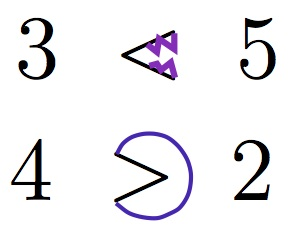
\includegraphics[scale=1]{inequal51.jpg}
\end{center}

Here is some terminology:  
\begin{itemize}
	\item $a>b$ means $a$ is greater than $b$.
	\item $a\geq b$ means $a$ is greater than or equal to $b$.
	\item $a<b$ means $a$ is less than $b$.
	\item $a\leq b$ means $a$ is less than or equal to $b$.
\end{itemize}	

Some things to remember with inequalities are that if  $0<a<b$, then $\frac{1}{a}>\frac{1}{b}$. Also, when you multiply or divide by negative numbers, the inequality sign switches.  Can you think of why this is the case? 


%\newpage
\section{Interval Notation}
We can use inequalities to describe \underline{sets} of numbers. For example, if we were to write $1<x<3$, the $x$ represents any number that is greater than $1$ and less than $3$. While there is nothing wrong with using inequalities to describe sets of numbers, we can also use a shorthand method called interval notation. Interval notation is preferred in college-level mathematics. Below are the corresponding inequalities and intervals:


\begin{itemize}
	\item   $a<x<b$ corresponds to $(a,b)$  
	\begin{center}
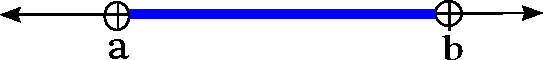
\includegraphics[scale=1]{ab1.pdf}
\end{center}

	\item   $a\leq x<b$ corresponds to $[a,b)$ 
		\begin{center}
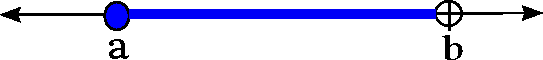
\includegraphics[scale=1]{ab2.pdf}
\end{center}
		\item  $a<x\leq b$ corresponds to $(a,b]$ 
			\begin{center}
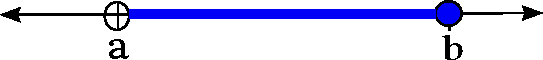
\includegraphics[scale=1]{ab3.pdf}
\end{center}
			\item  $a\leq x\leq b$ corresponds to $[a,b]$  
				\begin{center}
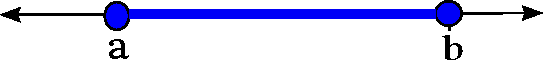
\includegraphics[scale=1]{ab4.pdf}
\end{center}

	\item    $a\leq x$ corresponds to $[a,\infty)$
		\begin{center}
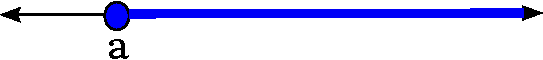
\includegraphics[scale=1]{ab5.pdf}
\end{center}
	\item  $x\leq b$ corresponds to $(-\infty, b]$ 
		\begin{center}
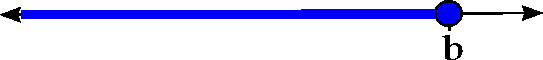
\includegraphics[scale=1]{ab6.pdf}
\end{center}
\end{itemize}	


Here are some comments:
\begin{itemize}
	\item  The smallest number always goes to the left and the largest number always goes to the right.  For example, $(2,8)$ is okay , but $(8,2)$ is not okay. 
	
	\item   If you {\bf{DON'T}} include the endpoint, use either ``('' or ``)'' 
		\item If you {\bf{DO}} include the endpoint, use either ``['' or ``]'' 
			\item   $\infty$ and $-\infty$ always use ``('' and ``)'' 
				\item  This is what WeBWork wants you to use (unless stated otherwise)  
					\item  If you have multiple intervals, you use a ``U'' to combine them: $-1\leq x<4$ or $x>9$ is represented by $$[-1,4)\cup (9,\infty)$$   
\end{itemize}

\vspace{1cm}







\everymath{\displaystyle}
\begin{exm}{}
What is the interval notation that corresponds to the following set of numbers?
\begin{itemize}
    \item $x>1$ or $x<-1$\vspace{3cm}
    \item $x\leq1$ or $x>-1$\vspace{3cm}
        \item All real numbers, $x$, so that $x\neq 1,2$\vspace{3cm}
    \item $x$ so that $x^2\neq 2$\vspace{3cm}
    \end{itemize}
\end{exm}\vskip10pt




\section{Review}
Recall the following facts about inequalities:
\begin{itemize}
	\item  $x\geq y$ is equivalent to $y\leq x$ 
 	\item   If $0<a<b$, then $\frac{1}{a}>\frac{1}{b}$
	\item  If $a<b$, then $-a>-b$
 \item Eat the biggest number
 \begin{center}
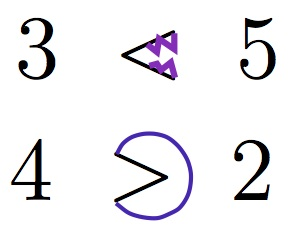
\includegraphics[scale=1]{inequal51.jpg}
\end{center}
\end{itemize}

\everymath{\displaystyle}
\begin{exm}{}Find all $x$ so that  $2x+5<4$. Provide your answer as both an inequality and in interval notation.
\end{exm}\vskip10pt

\begin{exmref}\label{2xplus10geq0}Find all $x$ so that  $2x+10 \geq 0$. Provide your answer as both an inequality and in interval notation.
\end{exmref}\vskip10pt




%\newpage
\begin{exm}{}Find all $x$ so that  $-3<-2x+5\leq 5$. Provide your answer as both an inequality and in interval notation.
\end{exm}\vskip10pt

\begin{exm}{}Find all $x$ so that  $4x-3\leq 2x+5$. Provide your answer as both an inequality and in interval notation.
\end{exm}\vskip10pt

\begin{exm}{}Find all $x$ so that  $-6<2x-4\leq 2$. Provide your answer as both an inequality and in interval notation.
\end{exm}\vskip10pt

%\newpage
\begin{exm}{}Find all $x$ so that  $-5\leq \frac{4-3x}{2}<1$. Provide your answer as both an inequality and in interval notation.
\end{exm}\vskip10pt

\begin{exm}{}Find all $x$ so that  $9+\frac{1}{3}x\geq4-\frac{1}{2}x$. Provide your answer as both an inequality and in interval notation.
\end{exm}\vskip10pt

%\newpage
\begin{exm}{}Find all $x$ so that  $4>\frac{2-3x}{7}\geq-2$. Provide your answer as both an inequality and in interval notation.
\end{exm}\vskip10pt


%\newpage
\renewcommand{\booksection}{Absolute Value Equations}
\renewcommand{\pageheader}{\booksection }
\section*{\LARGE \pageheader}
%\begin{concepts}
% \item  Solving linear absolute value equations
%\end{concepts}

\everymath{\displaystyle}
\begin{exm}{}Solve  $|x|=5$, with final answer not mentioning absolute value.
\end{exm}\vskip10pt

\begin{exm}{}Solve  $|u|=6$, with final answer not mentioning absolute value.
\end{exm}\vskip10pt

%\newpage

\begin{exm}{}Solve  $|x|-2= 5$
\end{exm}\vskip10pt

\begin{exm}{}Solve  $|x-2|= 5$
\end{exm}
\begin{bwarning}{}{}
Taking $|x -2| =5$ and adding $2$ on both sides does not lead to $|x|=7$. This instead leads to $|x -2|+2 = 7$, and unfortunately, the $-2$ inside the absolute value and the $+2$ outside the absolute value don't interact.
\end{bwarning}
{\bf Answer:} Replace every \fbox{$x-2$} with \fbox{$u$}
\[ |u| = 5 \]
State the values of $u$ which satisfy this equation.
\[ u= -5 \quad\text{or}\quad u=5\]
Replace every \fbox{$u$} with \fbox{$x-2$}
\[ x-2= -5 \quad\text{or}\quad x-2=5\]
Solve each equation independently
\[ x= -3 \quad\text{or}\quad x=7\]

\vskip10pt

%\newpage

\everymath{\displaystyle}

\begin{exm}{}Solve  $|x+8|= 10$
\end{exm}\vskip10pt

\begin{exm}{}Solve  $|3x-4|=5$
\end{exm}\vskip10pt


%\newpage
\everymath{\displaystyle}
\begin{exm}{}Solve  $3|4x+1|= -3$
\end{exm}\vskip10pt

\begin{exm}{}Solve  $\biggm|\frac{x}{2}-\frac{2}{3}\biggm|=4$
\end{exm}\vskip10pt

\begin{exm}{}Solve  $\biggm|\frac{x}{3}-12\biggm|= 10$
\end{exm}\vskip10pt


%\newpage

\begin{exm} Solve for $x$ in
\[
\left(\frac{|3(x^4-x^2)+1|-4}{5}-9\right)^2+4\left(\frac{|3(x^4-x^2)+1|-4}{5}-9\right)=21\]
\end{exm}
{\bf Answer:}
 Let $u=\frac{|3(x^4-x^2)+1|-4}{5}-9$.
 \[ u^2+4u=21\]
 \[u^2+4u-21=0\]
 \[(u+7)(u-3)=0\]
 \[u+7=0 \text{ or } u-3=0\]
 \[u=-7 \text{ or } u=3\]
 \[\frac{|3(x^4-x^2)+1|-4}{5}-9=-7 \quad\text{ or }\quad \frac{|3(x^4-x^2)+1|-4}{5}-9=3\]

\[\frac{|3(x^4-x^2)+1|-4}{5}=2 \quad\text{ or }\quad \frac{|3(x^4-x^2)+1|-4}{5}=12\]
\[|3(x^4-x^2)+1|-4=10 \quad\text{ or }\quad |3(x^4-x^2)+1|-4=60\]
\[|3(x^4-x^2)+1|=14 \quad\text{ or }\quad |3(x^4-x^2)+1|=64\]
 Let $m=3(x^4-x^2)+1$
\[|m|=14 \quad \text{ or } \quad |m|=64\]
\[m=14 \text{ or } m = -14 \quad \text{ or } \quad m=64 \text{ or } m = -64\]
 {\footnotesize\[3(x^4-x^2)+1=14 \text{ or } 3(x^4-x^2)+1 = -14  \text{ or }  3(x^4-x^2)+1=64 \text{ or } 3(x^4-x^2)+1 = -64\]}
 {\[3(x^4-x^2)=13 \text{ or } 3(x^4-x^2) = -15  \text{ or }  3(x^4-x^2)=63 \text{ or } 3(x^4-x^2) = -65\]}
 {\[x^4-x^2=\frac{13}{3} \text{ or } x^4-x^2 = -5  \text{ or }  x^4-x^2=21 \text{ or } x^4-x^2 = -\frac{65}{3}\]}
 {\[(x^2)^2-x^2=\frac{13}{3} \text{ or } (x^2)^2-x^2 = -5  \text{ or }  (x^2)^2-x^2=21 \text{ or } (x^2)^2-x^2 = -\frac{65}{3}\]}
 Let $s=x^2$
 {\[s^2-s=\frac{13}{3} \text{ or } s^2-s = -5  \text{ or } s^2-s=21 \text{ or } s^2-s = -\frac{65}{3}\]}
Now, solve these four quadratic equations (each by completing the square). Once values of $s$ are found, go replace $s$ with $x^2$.



%\newpage
\renewcommand{\booksection}{Absolute Value Inequalities}
\renewcommand{\pageheader}{\booksection }
\section*{\LARGE \pageheader}

\everymath{\displaystyle}
\begin{exm}{}Solve  $|x| \leq 3$, stating an answer without absolute values.
\end{exm}\vskip10pt
\begin{exm}{}Solve  $|x| \geq 3$, stating an answer without absolute values.
\end{exm}\vskip10pt
\begin{exm}{}Solve  $|x| < 3$, stating an answer without absolute values.
\end{exm}\vskip10pt
\begin{exm}{}Solve  $|r| > 3$, stating an answer without absolute values.
\end{exm}\vskip10pt
\begin{exmref}\label{uleq7}Solve  $|u| \leq 7$, stating an answer without absolute values.
\end{exmref}\vskip10pt

%\newpage

\begin{exm}{}Solve  $|x| + 3 \leq 10$
\end{exm}\vskip10pt


\begin{exm}{}Solve  $|x + 3| \leq 10$
\end{exm}
\begin{bwarning}{}{}
Taking $|x + 3| \leq 10$ and subtracting $3$ on both sides does not lead to $|x| \leq 7$. This instead leads to $|x + 3|-3 \leq 7$, and unfortunately, the $+3$ inside the absolute value and the $-3$ outside the absolute value don't interact.
\end{bwarning}
How can we use Example~\ref{uleq7}?
\vskip10pt



%\newpage

\begin{exm}{}Solve  $|3x-4|<5$
\end{exm}\vskip10pt

\begin{exmref}\label{absx2geq10}Solve  $|x-2| \geq 10$
\end{exmref}\vskip10pt

%\newpage
\everymath{\displaystyle}
\begin{exm}{}Solve  $|x-2| + 2 \geq 10$
\end{exm}\vskip10pt

\begin{exm}{}Solve  $-4|4x+1|\leq -3$
\end{exm}\vskip10pt

%\newpage
\everymath{\displaystyle}
\begin{exm}{}Solve  $\biggm|\frac{x}{2}-\frac{2}{3}\biggm|\geq -4$
\end{exm}\vskip10pt

\begin{exm}{}Solve  $\biggm|12-\frac{x}{3}\biggm|< 10$
\end{exm}\vskip10pt







%\newpage
\renewcommand{\booksection}{Functions}
\renewcommand{\pageheader}{\booksection }
\section*{\LARGE \pageheader}

\section{Functions }

\begin{bdefinition}{Function}{function}
A function is a rule that describe exactly one output for each input.
\end{bdefinition}
Each input has \underline{one} output. We cannot have an input with \underline{two} outputs, and we cannot have an input with \underline{no} outputs.

\begin{exm}
\begin{center}
    \begin{overpic}{math-practice-test-on-function.jpg}
\put(15,55){\textcolor{red}{NO}}
\put(15,-5){\textcolor{red}{NO}}
\put(52,55){\textcolor{green}{YES}}
\put(52,-5){\textcolor{green}{YES}}
\put(81,55){\textcolor{red}{NO}}
\put(81,-5){\textcolor{red}{NO}}
\end{overpic}
\end{center}
\end{exm}

A \underline{function} consists of three things: 
\begin{itemize}
	\item A set of inputs (stuff that goes into the function) called the {\bf domain}
		\item  A set of outputs (stuff that comes out of the function) called the {bf range} 
		\item  A rule assigning each input to exactly one output 
\end{itemize}
\begin{center}
  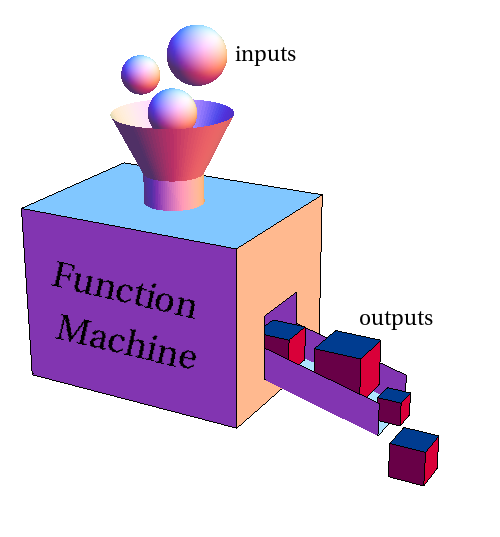
\includegraphics[scale=.4]{function_machine.png} 
\end{center}	

We have specific notation for functions: 
\begin{center}
  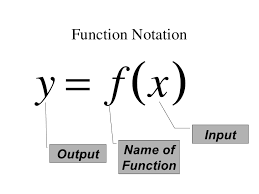
\includegraphics[scale=1]{download.png} 
\end{center}	

%\newpage

\begin{exm}{If $f(x)=x^2+6$, find $f(10)$}
\end{exm}
{\bf Answer:} $f(10)=(10)^2+6$.

After simplifying, we have $f(10)=100+6$ and simplifyng further, $f(10)=106$.
\begin{blanguage}{}{}
Use the words \underline{input} and \underline{output} when talking about a function.
\end{blanguage}
\begin{exm}
For the function $f(x)=x^2+6$,\\ if the input is $10$, the output is $106$.\\
This is summarized by writing $f(10)=106$.
\end{exm}
\begin{exm}
For the function $f(x)=x^2+6$,\\ if the input is $5$, the output is $31$.\\
This is summarized by writing $f(5)=31$.
\end{exm}

\begin{blanguage}{Function}{fofx}
When seeing/writing $f(x)$ say ``$f$ of $x$'' and do not skip the word \underline{of}. Similarly, $f(5)$ should be said ``$f$ of $5$''. If you skip the \underline{of}, it leads to the error of thinking we have ``$f$ times $5$'' but there is no multiplication going on between $f$ and $5$ at all!
\end{blanguage}


\vskip16pt
\hrule
\vskip16pt

\begin{exm}
Given $f(x)=10^x+6x$ find $f(2)$
\end{exm}
{\bf Answer:} $f(2) = 10^2+6(2)$. Simplified, $f(2)=112$. In words, the input $2$ leads to the output $112$.
\begin{bwarning}{}{}
In the last example, we wrote \fbox{$f(2)=10^2+6(2)$} which is correct.\\
Writing \fbox{$f(x)=10^2+6(2)$} is incorrect.
\end{bwarning}

\begin{bmethod}{Finding the output for an input}{}
{\bf Task:} $f(x)=10^x+6x$ find $f(2)$.\vskip10pt

{\bf How to restate the task:} Notice the $2$ inside parentheses.

While writing \fbox{$f(x)=10^x+6x$} replace every \fbox{$x$} you see with~\fbox{$2$}. This even applies to the $x$ that is on the left of the equal sign.
\end{bmethod}

%\newpage


\includegraphics[width=3in]{oodle}

\vskip10pt


\includegraphics[width=3in]{chomponzoo}
\vskip10pt
\vskip10pt

%\newpage

Replace every \fbox{vowel} in \fbox{your name} with \fbox{oodle}

\vskip40pt

Given $f(x)=10^x+6x$ to find $f(2)$ you must:\\
Replace every \fbox{\phantom{...AAAAA.A........}} in \fbox{\phantom{....A..AAAAA......}} with \fbox{\phantom{......AA......}}

\vskip20pt

Given $f(x)=10^x+6x$ to find $f(c)$ you must:\\
Replace every \fbox{\phantom{...AAAAA.A........}} in \fbox{\phantom{....A..AAAAA......}} with \fbox{\phantom{......AA......}}

\vskip80pt

Given $f(x)=x^2+x+3$ to find $f(a+h)$ you must:\\
Replace every \fbox{\phantom{...AAAAA.A........}} in \fbox{\phantom{....A..AAAAA......}} with \fbox{\phantom{......AA......}}

\vskip20pt

Given $f(x)=x^2+x+3$ to find $f(x+h)$ you must:\\
Replace every \fbox{\phantom{...AAAAA.A........}} in \fbox{\phantom{....A..AAAAA......}} with \fbox{\phantom{......AA......}}


%\newpage

\begin{exm}{If $f(x)=x^2+x+3$, find $f(3)$, $f(c)$, and $f(x+h)$}
\end{exm}\vskip10pt

%\newpage
 Notice that if you are asked to find $f(x+h)$, {\it all} of $x+h$ is put into the function.

\everymath{\displaystyle}
\begin{exm}{If $f(x)=x^2$, find $f(x+h)$ and $f(x)+h$.}
\end{exm}\vskip10pt
 
\begin{bwarning}{Function does not ``distribute''}{}
$f(x+h) \not= f(x)+f(h)$
\end{bwarning}

%\newpage


\begin{exm}
Given the function $f(x)=3x+1$, find $\dfrac{f(x+h)-f(x)}{h}$.
\end{exm}
We see that 
$$f(x+h)=3(x+h)+1 ~~~~\mbox{and}~~~~~ f(x)=3x+1.$$
Therefore, 
\begin{align*}
    \frac{f(x+h)-f(x)}{h}&=\frac{3(x+h)+1-(3x+1)}{h}\\
    &=\frac{3x+3h+1-3x-1}{h}\\
    &=\frac{3h}{h}\\
    &=3\\
\end{align*}

\vskip10pt

%\begin{exm}
%For the function $f(x)=\sqrt{x-2}$, find $\dfrac{f(x+h)-f(x)}{h}$
%\end{exm}
%We see that 
%	$$f(x+h)=\sqrt{x+h-2}~~~~\mbox{and}~~~ f(x)=\sqrt{x-2}$$
% Therefore, 
%\begin{align*}
%\frac{f(x+h)-f(x)}{h}&=\frac{\sqrt{x+h-2}-\sqrt{x-2}}{h}\\
%&=\frac{\sqrt{x+h-2}-\sqrt{x-2}}{h}\left(\frac{\sqrt{x+h-2}+\sqrt{x-2}}{\sqrt{x+h}-2+\sqrt{x-2}}\right)\\
%&=\frac{h}{h(\sqrt{x+h}-2+\sqrt{x-2})}\\
%&=\frac{1}{\sqrt{x+h}-2+\sqrt{x-2}}\\
%\end{align*}

\begin{exm}
Given the function $f(x)=\frac{1}{x}$, find $\dfrac{f(x+h)-f(x)}{h}$
\end{exm}
$$f(x+h)=\frac{1}{x+h} ~~~~\mbox{and}~~~~ f(x)=\frac{1}{x}$$ 
So, 
\begin{align*}
\frac{f(x+h)-f(x)}{h}&=\frac{\frac{1}{x+h}-\frac{1}{x}}{h}\\   
	&=\frac{1}{h}\left(\frac{x}{x(x+h)}-\frac{x+h}{x(x+h)}\right)\\
 &=\frac{-1}{x(x+h)}\\
\end{align*}

\vskip10pt

%\newpage
\everymath{\displaystyle}
%\begin{exm}{For the function $f(x)=\frac{1}{\sqrt{4-x^2}}$, find $\dfrac{f(x+h)-f(x)}{h}$}
%\end{exm}\vskip10pt

%\begin{exm}{For the function $g(x)=\sqrt{x^2-4}$, find $\dfrac{f(g+h)-g(x)}{h}$}
%\end{exm}\vskip10pt

%%\newpage
%\everymath{\displaystyle}
%\begin{exm}{For the function $f(x)=\frac{1}{\sqrt{x-2}}$, find $\dfrac{f(x+h)-f(x)}{h}$}
%\end{exm}\vskip10pt

\begin{exm}Given the function $f(x)=-10x^2+3x$, find $\dfrac{f(x+h)-f(x)}{h}$ and simplify\footnote{In {\bf business}, $f(x)=-10x^2+3x$ is typical of a {\bf revenue function} looks. The expression we found is called the {\bf average revenue}}. 
\end{exm}\vskip10pt



%\newpage


\subsection{Domains}
  The set of numbers that make sense in the function is called the domain. 
 Unless the domain is given to you, assume it's as large as possible.  
 For example, if $f(x)=\sqrt{x}$,  $f(-2)=\sqrt{-2}$ doesn't make sense so $-2$ is not in the domain of this function.  

\begin{bmethod}{How to find domain}{domain}
\begin{itemize}
\item Avoid diving by zero. (In other words, what values of $x$ cause the denominator to be zero? We must exclude these $x$-values.)
\item Avoid square rooting a negative number. Rephrased, we want/need what we are square rooting to be greater than or equal to $0$. In other words, we need the content \emph{inside} a square root to be $\geq0$.
\end{itemize}
\end{bmethod}

\begin{exm}
Find the domain of $f(x) = \sqrt{2x+10}$
\end{exm}
{\bf Answer:} We need $2x+10 \geq 0$. In Example~\ref{2xplus10geq0}, we saw the answer to this was $[-5,\infty)$. So the domain of $f$ is $[-5,\infty)$.

\begin{exm}[Follow up]
If $f(x) = \sqrt{2x+10}$ find $f(-3)$
\end{exm}
{\bf Note:} Though the $x$-value $x=-3$ is negative, we are not square rooting $x$ itself. We are square rooting $2x+10$. We already note that the domain was found to be $[-5,\infty)$, and $-3$ is in this interval.
\vskip50pt

\begin{exm}
Find the domain of $f(x) = \sqrt{|x-2| - 10}$
\end{exm}
{\bf Answer:} We need $|x-2|-10 \geq 0$. So $|x-2| \geq 10$. We solved this inequality in Example~\ref{absx2geq10} and got $(-\infty,-8) \cup (12,\infty)$ as our answer. Thus, the domain of $f$ is $(-\infty,-8) \cup (12,\infty)$.

\begin{exm}
Find the domain of $f(x) = \frac{x^2+5x+6}{x^2+2x-24}$
\end{exm}

%\newpage

\begin{exm}
Find the domain of $f(x) = \frac{2x + \sqrt{3x+21}}{x^2+2x-24}$
\end{exm}

%\newpage

\subsection{Graphs of Functions}
Given a function $f$, a point on the graph of $f$ is given by $(x,f(x))$. The $x$-axis is the ``input'' axis and the $y$-axis is the ``output'' axis. In other words:
\begin{bconcept}{}{}
$f(a)=b$ if and only if the point $(a,b)$ is on the graph of $f$
\end{bconcept}

Lots of graphs do not represent functions. A graph must pass the \underline{Vertical Line Test (VLT)} in order to be a graph of a function. The  \underline{Vertical Line Test} states that every vertical line must pass through the graph at {\it most} one time.

\begin{exm}
Find three points on the graph of $f(x) = x^2+6$
\end{exm}

%\newpage

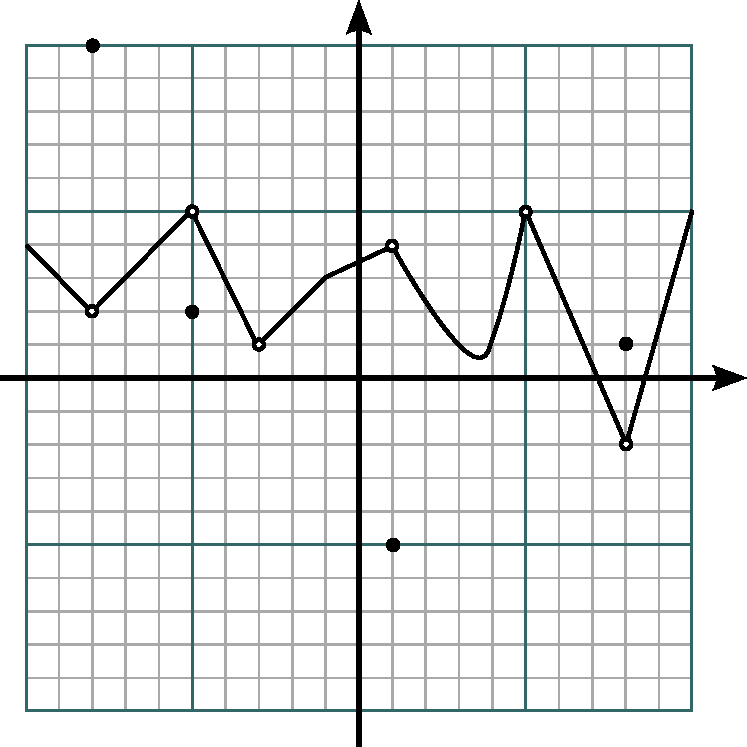
\includegraphics[width=4in]{twosided-limits}

\begin{exm}
The graph above passes the Vertical Line Test, so let us say that this graph introduces to us a function $y=f(x)$. Find $f(6)$.
\end{exm}
Note: we have done this task using different language in Example~\ref{interpolation}.


%\newpage

\subsection{Linear Functions}
 A {\bf{linear function}} is a function of the form: $$f(x)=mx+b.$$  The value $m$ is the slope of the line and $b$ is the $y$-intercept.Here, the $f(x)$ is the output just like $y$ in the equation $y=mx+b$.  

%\newpage
\everymath{\displaystyle}
\begin{exm}{Let $f$ be a linear function given by $f(x)=3x+5$. Find $f(0), f(2), f(-10)$}
\end{exm}\vskip10pt

\begin{exm}{Determine if the function $f(x)=\frac{x+1}{5}$ is a linear function. If so, identify the slope and $y$-intercept.}
\end{exm}\vskip10pt

\everymath{\displaystyle}
\begin{exm}{Determine the point of intersection of the graphs of the functions $f(x)=3x+1$ and $g(x)=-2x+5$.}
\end{exm}\vskip10pt

\begin{exm}{A pond is being filled at a rate of 10 gallons per minute. Initially the pond contains 300 gallons. Find a linear function that models this situation. Then, determine when the pond will contain 1300 gallons. }
\end{exm}\vskip10pt

%\newpage
\begin{exm}{ Find a linear function whose graph passes through $(3,-2)$ and $(2,0)$.}
\end{exm}\vskip10pt



%\newpage

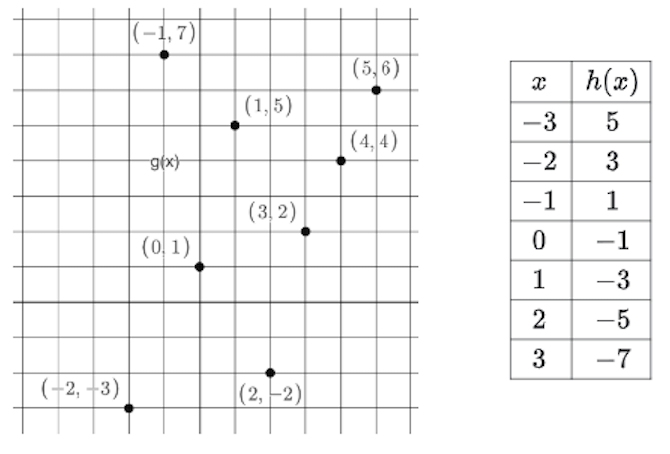
\includegraphics[width=5.0in]{warnberg-pre}

The picture in the upper left shows the graph of a function called $g(x)$ while the table on the right shows the inputs/outputs for a function called $h(x)$.

\begin{exm}
Find $g(2)$
\end{exm}
\vskip10pt
\begin{exm}
Find $h(3)$
\end{exm}
\vskip10pt
\begin{exm}
Find $h(3)+g(5)$
\end{exm}
\vskip10pt
\begin{exm}
Find $h(1)+g(2) + 10^{g(3)} + 10\,h(-3)$
\end{exm}
\vskip10pt
\begin{exm}
For what value(s) of $x$ is $g(x)$ equal to $2$? How is this question different from the first question on this page?
\end{exm}
\vskip10pt

%\newpage
\renewcommand{\booksection}{Quadratic Functions}
\renewcommand{\pageheader}{\booksection }
\section*{\LARGE \pageheader}

 A {\bf Quadratic Function} is a function whose rule is a quadratic expression. One such example would be:  $$f(x)=ax^2+bx+c, ~~~~ a\neq 0.$$
There are many ways to represent a quadratic expression. Here is another example of a quadratic function: 
		$$f(x)=a(x-h)^2+k.$$
  This last example is called the \underline{vertex form} of a quadratic function.  Every quadratic function can be written in both standard and vertex form. 	



\everymath{\displaystyle}
\begin{exm}{}Rewrite the function $f(x)=(x-2)^2+1$ in standard form
\end{exm}\vskip10pt

\begin{exm}{}Rewrite the function $f(x)=-3(x+1)^2-7$ in standard form.
\end{exm}\vskip10pt
%\newpage




\section{Standard Form to Vertex Form}
Rewriting a quadratic function from standard form to vertex form is a bit more challenging. However, the good news is that there is a formula we can use. This will be given at the end of this section. 
 Suppose we are given the quadratic function $f(x)=ax^2+bx+c$. We want to change this to $y=ax^2+bx+c$,subtract $c$,and divide by $a$.This gives you: 
		$$\frac{y-c}{a}=x^2+\frac{b}{a}x.$$ 
  
  We do this so that we can complete the square. We do this by adding $\left(\frac{b}{2a}\right)^2$ to both sides: 
	 $$\frac{y-c}{a}+\left(\frac{b}{2a}\right)^2=x^2+\frac{b}{a}x+\left(\frac{b}{2a}\right)^2$$  
		$$\frac{y-c}{a}+\left(\frac{b}{2a}\right)^2=\left(x+\frac{b}{2a}\right)^2$$
 Now, we want to solve for $y$: $$\frac{y-c}{a}=\left(x+\frac{b}{2a}\right)^2-\left(\frac{b}{2a}\right)^2$$
	    $$y-c=a\left(x+\frac{b}{2a}\right)^2-\frac{b^2}{4a}$$
	  $$y=a\left(x+\frac{b}{2a}\right)^2+c-\frac{b^2}{4a}$$
 Our last step is to write $y$ as $f(x)$: $$f(x)=a\left(x+\frac{b}{2a}\right)^2+c-\frac{b^2}{4a}.$$
You will; notice that given a standard form of a quadratic function, $f(x)=ax^2+bx+c$, the corresponding vertex form is:  
$$f(x)=a\left(x+\frac{b}{2a}\right)^2+c-\frac{b^2}{4a}.$$









\everymath{\displaystyle}
\begin{exm}{}Write $f(x)=-x^2-4x+5$ in vertex form.
\end{exm}\vskip10pt

%\newpage
\begin{exm}{}Rewrite the function $f(x)=x^2+8x-2$ in vertex form.
\end{exm}\vskip10pt

\begin{exm}{}Rewrite the function $f(x)=2x^2+3x-1$ in vertex form.
\end{exm}\vskip10pt



\renewcommand{\booksection}{ Graphing Quadratic Functions  }    % Need to separately identify this for
                                    % example labeling
\renewcommand{\pageheader}{\booksection }
\resetcounters

\section*{\LARGE \pageheader}

$$f(x)=ax^2+bx+c~~~~~~~~~~~~~~~~~~~~~~~f(x)=a(x-h)^2+k$$


%\begin{concepts}
% \item  Domain and range of quadratic functions
%	\item Vertex of a quadratic function 
%	\item Min/Max values of a quadratic
%\end{concepts}
%\vspace{1cm}



\section{Vertex Form}
When working with quadratic functions, we prefer to use the vertex form for many reasons such as it allows us to find the range and min/max values. Given a quadratic in vertex form $f(x)=a(x-h)^2+k$,  the vertex is the point $(h,k)$.

\begin{center}
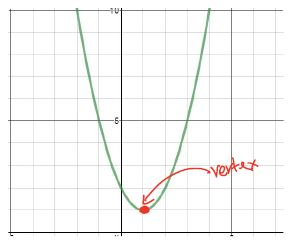
\includegraphics[scale=.4]{vertex1.JPG}
\end{center}
We also know that
\begin{itemize}
		\item if $a<0$, then the quadratic opens downwards,  
		\item if $a>0$, then the quadratic opens upwards.  
\end{itemize}	


\everymath{\displaystyle}
\begin{exm}{}Sketch the graph of $f(x)=(x-2)^2+1$. Then, find the domain and range of $f(x)$.
\end{exm}\vskip10pt

%\newpage
\begin{exm}{}Sketch the graph of $y=-x^2-3$. Then, find the domain and range of $y$.
\end{exm}\vskip10pt

\begin{exm}{}Sketch the graph of $f(x)=x^2+2x+5$. Then, find the domain and range of $f(x)$.
\end{exm}\vskip10pt

%\newpage
\subsection{Standard Form to Vertex Form}
 Given a quadratic in standard form, $f(x)=ax^2+bx+c$, the vertex is given by $$(h,k)=\left( \frac{-b}{2a}  , f\left(\frac{-b}{2a}\right)   \right)$$
 This allows you to write a standard quadratic in vertex form without completing the square. 
The vertex is a point on the graph of a function, if you can remember the $x$-coordinate is $\frac{-b}{2a}$, then you can find the $y$-coordinate by putting this $x$-value into the function $f$ to get a $y$-value.


\everymath{\displaystyle}
\begin{exm}{}Write $f(x)=-x^2+4x+5$ in vertex form. Graph the function $f(x)$. Then state which $x$-value leads to the largest $y$-value\footnote{In business, the function $f(x)=-x^2+4x+5$ is the typical look of a {\bf profit function}. Finding the point on the graph which has the largest $y$-value is maximizing the profit of a business.}.
\end{exm}\vskip10pt

%\newpage
\begin{exm}{}Graph the function $f(x)=x^2-4x+5$. Then, find the minimum of $f(x)$. 
\end{exm}\vskip10pt


\everymath{\displaystyle}
\begin{exm}{}Find the $x$ and $y$ intercepts of  $f(x)=x^2-4x+5$.
\end{exm}\vskip10pt

\begin{exm}{}Graph the function $h(x)=-4x^2+9x+a$. Determine the maximum of $g(x)$.
\end{exm}\vskip10pt

%\newpage
\everymath{\displaystyle}
\begin{exm}{}Find the quadratic that has vertex $(2,4)$ and passes through the point $(1,2)$.
\end{exm}\vskip10pt

\everymath{\displaystyle}
\begin{exm}{}Find the quadratic with a minimum $y=3$, that is symmetric about the line $x=1$ and passes through the point $(5, 9)$.
\end{exm}\vskip10pt

Let's suppose that we want to find $x$ so that $x^2-4x-15\leq6$. We can use technology to see the values of $x$ that satisfy this inequality. However, by rewriting $x^2-4x-15<6$ as $x^2-4x-21<0$, we can factor this quadratic to get  $$(x-7)(x+3)<0$$
It is tempting to solve this similar to a quadratic, however we must use a sign chart and test values. 

\begin{bmethod}{Solving a polynomial inequality}{}
\begin{itemize}
\item Set one side of the inequality to $0$  
\item  Find the values of $x$ that make the quadratic equal to $0$   
		\item  Put these numbers on a number line 
	\item Find numbers in each of the regions
\item  Plug the test values into the quadratic  
\item      Determine when the quadratic is positive or negative 
\item      Choose the region that satisfies the inequality.
\item If there are multiple separate intervals, write down intervals using $\cup$
\end{itemize}
\end{bmethod}

\begin{exm}
\begin{itemize}
	\item  Set one side of the inequality to $0$  
	$$x^2-4x-21<0$$
	
	\item  Find the values of $x$ that make the quadratic equal to $0$   
	$$(x-7)(x+3)=0\leftrightarrow x=7,~~x=-3$$
	
		\item  Put these numbers on a number line 
				\begin{center}
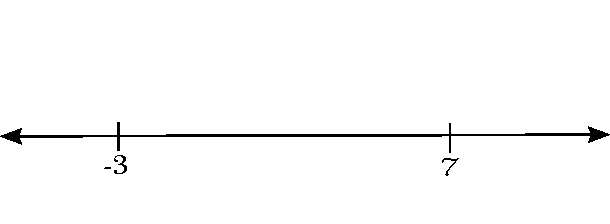
\includegraphics[scale=.9]{371.pdf}
\end{center}

	\item Find numbers in each of the regions
				\begin{center}
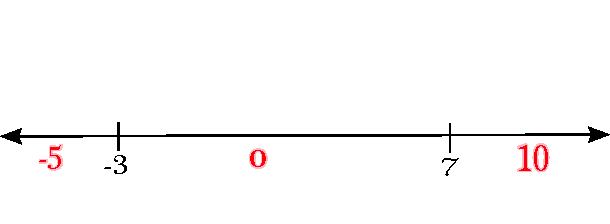
\includegraphics[scale=.9]{372.pdf}
\end{center}

\item  Plug the test values into the quadratic  

				\begin{center}
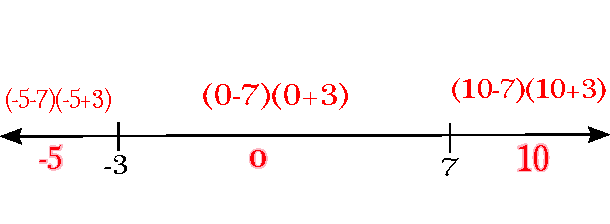
\includegraphics[scale=.9]{373.pdf}
\end{center}

\item      Determine when the quadratic is positive or negative 
				\begin{center}
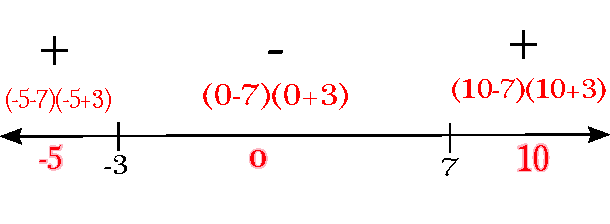
\includegraphics[scale=.9]{374.pdf}
\end{center}

\item      Choose the region that satisfies the inequality 
				\begin{center}
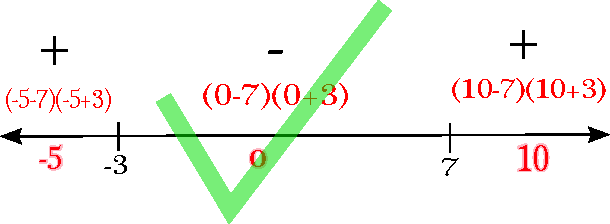
\includegraphics[scale=.9]{375.pdf}
\end{center}

\item For this problem, the answer is $(-3,7)$.
\end{itemize}	
\end{exm}

%\newpage
\everymath{\displaystyle}
\begin{exm}{Solve $x^2+4x+3\leq 0$ }
\end{exm}\vskip10pt

\begin{exm}{Solve $x(3x-1)\geq 4$ }
\end{exm}\vskip10pt

%\newpage
\begin{exm}{Solve $2x^3-3x^2-2x+3\leq 0$.}
\end{exm}\vskip10pt



%\newpage
\renewcommand{\booksection}{Polynomial functions, zeroes}
\renewcommand{\pageheader}{\booksection }
\section*{\LARGE \pageheader}
%\begin{concepts}
% \item  Distributive property
%	\item leading term, roots, degree
%\end{concepts}
%\vspace{1cm}


A polynomial function is a function of the form: $$f(x)=a_nx^n+a_{n-1}x^{n-1}+a_{n-2}x^{n-2}+\dots a_2x^2+a_1x^1+a_0,$$ where the $a_i$'s are constants and the exponents, $n$, are non-negative integers. The largest exponent of $x$ is called the \underline{\bf degree} of the polynomial $f$. 
The coefficient (ie the number) in front of the term with the highest exponent for $x$ is called the  \underline{\bf leading coefficient} for the polynomial $f$.  


\everymath{\displaystyle}
\begin{exm}{}Identify the degree and leading coefficient for the polynomials $f(x)=27x^4+\sqrt{\pi}x-100x^{10}$, $g(x)=x+2$ and $h(x)=x^5+x^4+x^3+x^2+x^1+1$.
\end{exm}\vspace{6cm}

Suppose that the polynomial is in factored form: $$f(x)=a(x-r_1)^{k_1}(x-r_2)^{k_2}\dots(x-r_j)^{k_j}$$
We can easily graph these polynomials know the $r_i$'s, leading coefficient, and degree.

\section{Factors of Polynomials}
 Suppose that the polynomial is in factored form: $$f(x)=a(x-r_1)^{k_1}(x-r_2)^{k_2}\dots(x-r_j)^{k_j}$$  We know that $r_i$ are roots. This means:     \begin{itemize}
	\item $(r_i,0)$ is on the graph of $f$ ($r_i$ are $x$-intercepts)   
	\item  $f(r_i)=0$  
\end{itemize}
The corresponding exponent, $k_i$, for the factor $(x-r_i)$ is called the \underline{\bf multiplicity} of the root $r_i$.  

%\newpage
\everymath{\displaystyle}
\begin{exm}{Is $x+4$ a factor of $x^3+64$? Find all roots with multiplicities of $x^3+64$.}
\end{exm}\vskip10pt

\begin{exm}{Give an example of a polynomial of degree $7$ with roots at $x=-3, 0, 1, 5$. }
\end{exm}\vskip10pt

%\newpage



\subsection{Terminology}
Let's go over some vocabulary. The words {\bf zero}, {\bf root}, and {\bf $x$-intercept} all mean the same thing: Given a polynomial $p(x)$, a zero is {\it any} value of $x$ so that $p(x)=0$. A zero is also  {\it any} value of $x$ where the graph of $p(x)$ touches/crosses the $x$-axis.



%\newpage

\renewcommand{\booksection}{ Graphing Polynomials  }
\renewcommand{\pageheader}{\booksection }
\resetcounters

\section*{\LARGE \pageheader}

\begin{intro}
\begin{abstract}
%$$\lim_{x\to a}f(x)=L$$
\end{abstract}
\end{intro}
%
%
%\begin{concepts}
% \item  Degree of polynomial
%	\item Roots and multiplicities of polynomials
%	\item graphing polynomials
%\end{concepts}
%\vspace{1cm}



\section{Vocabulary of Polynomials}
 A polynomial function is a function of the form: $$f(x)=a_nx^n+a_{n-1}x^{n-1}+a_{n-2}x^{n-2}+\dots a_2x^2+a_1x^1+a_0,$$ where the $a_i$'s are constants and the exponents, $n$, are non-negative integers.  The largest exponent of $x$ is called the \underline{\bf degree} of the polynomial $f$. The coefficient (ie the number) in front of the term with the highest exponent for $x$ is called the  \underline{\bf leading coefficient} for the polynomial $f$. 

 Polynomials are {\bf continuous functions}. This means that you can draw it without picking up your pencil.    

\begin{center}
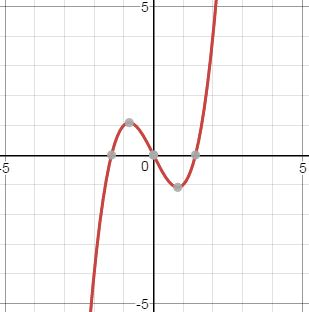
\includegraphics[scale=.75]{poly.jpg}
\end{center}

%\newpage
\subsection{Degree of Polynomials}
Suppose that the degree of a polynomial is {\it even}, then we can say something about the ends of the graph:   
	\begin{figure}[ht]
\begin{center}
\begin{overpic}[scale=.5]{poly_even.pdf}
\put(10, 0){$a_n>0$}
\put(70,0){$a_n<0$}
\end{overpic}
\end{center}
\end{figure}

Suppose that the degree of a polynomial is {\it odd} then we can say something about the ends of the graph:   
		\begin{figure}[ht]
\begin{center}
\begin{overpic}[scale=.5]{poly_odd.pdf}
\put(10, 0){$a_n>0$}
\put(70,0){$a_n<0$}
\end{overpic}
\end{center}
\end{figure}
Here, the $a_n$ represents the leading coefficient for $f$.





\section{Factors of Polynomials}
 Suppose that the polynomial is in factored form: $$f(x)=a(x-r_1)^{k_1}(x-r_2)^{k_2}\dots(x-r_j)^{k_j}.$$  
 We know that $r_i$ are roots. This means the points $(r_i,0)$ are on the graph of $f$ ($r_i$ are $x$-intercepts) and  $f(r_i)=0$. 
 The corresponding exponent, $k_i$, for the factor $(x-r_i)$ is called the \underline{\bf multiplicity} of the root $r_i$. 

It turns out that if $r_i$ has multiplicity that is {\it even}, then the graph looks like teh graph below  near the root $r_i$. In other words, the graph touches, but does not cross the $x$ axis.  
\begin{center}
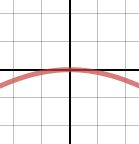
\includegraphics[scale=.5]{mult1.jpg}\hspace{60pt}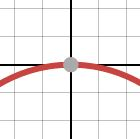
\includegraphics[scale=.5]{mult2.jpg}
\end{center}  

However, if $r_i$ has multiplicity that is {\it odd}, then the graph crosses the $x$ axis near $r_i$, similar to the graph below. 
\begin{center}
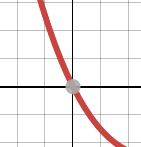
\includegraphics[scale=.5]{mult3.jpg}\hspace{60pt}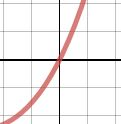
\includegraphics[scale=.5]{mult4.jpg}
\end{center}  



\subsection{Degrees of Polynomials}
Suppose that the polynomial is in factored form: $$f(x)=a(x-r_1)^{k_1}(x-r_2)^{k_2}\dots(x-r_j)^{k_j}.$$   We can find the degree of the polynomial $f$ by summing up all of the multiplicities: $$k_1+k_2+k_3+\dots k_{j}.$$ The leading coefficient for the polynomial $f$ is the number $a$. 


\everymath{\displaystyle}
\begin{exm}{Sketch the graph of $f(x)=x^2(x-1)(x-3)^2$}
\end{exm}\vskip10pt

\begin{exm}{Sketch the graph of $f(x)=-x^2-4x^4$}
\end{exm}\vskip10pt

%\newpage

\everymath{\displaystyle}
\begin{exm}Sketch the graph of $f(x)=(x^2-2)(x+7)(x-4)$ %$x^4+3x^3-30x^2-6x+56$
\end{exm}\vskip10pt







%\newpage
\renewcommand{\booksection}{Graph Transformations}
\renewcommand{\pageheader}{\booksection }
\section*{\LARGE \pageheader}

%
%\begin{concepts}
% \item  Vertical and horizontal shifts
%	\item Vertical and horizontal stretches
%	\item Reflections
%\item Even and Off functions
%\item Piece-wise functions
%
%\end{concepts}
%\vspace{1cm}



\section{Graph Transformations}
Given a function $f$, a point on the graph of $f$ is given by $(x,f(x))$.    The $x$-axis is the ``input'' axis and the $y$-axis is the ``output'' axis.   

The old method of graphing: take different values of $x$ and find the corresponding $y$ ($f(x)$) values, plot points, then sketch a graph. This is the least preferred method because it takes too much time and is not accurate. The new method is to use base graphs and modify them accordingly




\noindent {\bf Vertical transformations}\\Our example uses $f(x)=x^2$. Because $(a,b)$ is on the graph of $y=f(x)$ if and only if $f(a)=b$, we get...

\begin{center}
\begin{tabular}{|c|c|c|c|}\hline

& $y=f(x)$ original & & $y=f(x)+c$\\
& Ex: $y=x^2$ original & &Ex: $y=x^2+1$ \\
\begin{tikzpicture}
\node at (0,3.0) {$y=f(x)$};
\node at (0,2.6) {vs.};
\node at (0,2.2) {$y=f(x)+c$};
\node at (0,0) {\phantom{.}};
\end{tikzpicture}
&
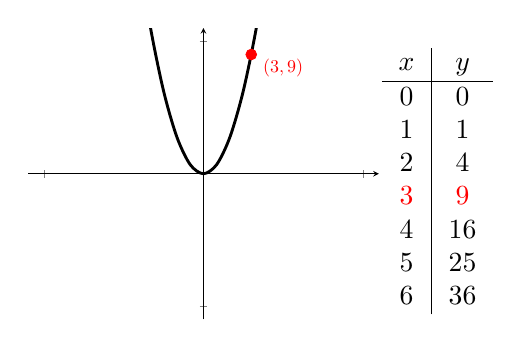
\begin{tikzpicture}[scale=0.65]
    \begin{axis}[
    axis x line=center,
    axis y line=center,
    ytick={-10,10},
    yticklabels={},
    xtick={-10,10},
    xticklabels={},
    xmin=-11, xmax=11, ymin=-11, ymax=11,
    ]
\plot[domain=-10:10, smooth, ultra thick, black]{x^2};
\filldraw[red] (axis cs:3,9) circle(3pt);
\node[red] at (axis cs: 5,8) {$(3,9)$};
\end{axis}
\node[anchor=north] at (8,5.5) {
\begin{tabular}{c|c}
$x$ & $y$ \\\hline
$0 $ & $0 $ \\
$1 $ & $1 $ \\
$2 $ & $4 $ \\
{\color{red}$3$} & ${\color{red}9} $ \\
$4$ & $16 $ \\
$5$ & $25 $ \\
$6$ & $36$ \\
\end{tabular}
};
\end{tikzpicture}
&
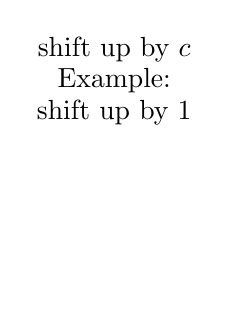
\begin{tikzpicture}
\node at (0,3.0) {shift up by $c$};
\node at (0,2.6) {Example:};
\node at (0,2.2) {shift up by $1$};
\node at (0,0) {\phantom{.}};
\end{tikzpicture}
&
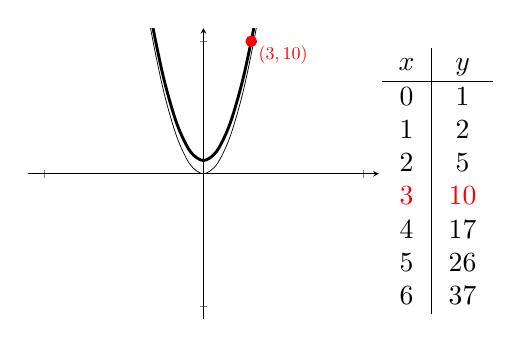
\begin{tikzpicture}[scale=0.65]
    \begin{axis}[
    axis x line=center,
    axis y line=center,
    ytick={-10,10},
    yticklabels={},
    xtick={-10,10},
    xticklabels={},
    xmin=-11, xmax=11, ymin=-11, ymax=11,
    ]
\plot[domain=-10:10, smooth]{x^2};
\plot[domain=-10:10, smooth, ultra thick, black]{x^2+1};
\filldraw[red] (axis cs:3,10) circle(3pt);
\node[red] at (axis cs: 5,9) {$(3,10)$};
\end{axis}
\node[anchor=north] at (8,5.5) {
\begin{tabular}{c|c}
$x$ & $y$ \\\hline
$0 $ & $1 $ \\
$1 $ & $2 $ \\
$2 $ & $5 $ \\
{\color{red}$3$} & ${\color{red}10} $ \\
$4$ & $17 $ \\
$5$ & $26 $ \\
$6$ & $37$ \\
\end{tabular}
};
\end{tikzpicture}
\\\hline
\end{tabular}
\end{center}


\begin{center}
\begin{tabular}{|c|c|c|c|}\hline
& $y=f(x)$ original &&  $y=f(x)-c$\\
& Ex: $y=x^2$ original && Ex: $y=x^2-1$\\
\begin{tikzpicture}
\node at (0,3.0) {$y=f(x)$};
\node at (0,2.6) {vs.};
\node at (0,2.2) {$y=f(x)-c$};
\node at (0,0) {\phantom{.}};
\end{tikzpicture}
&
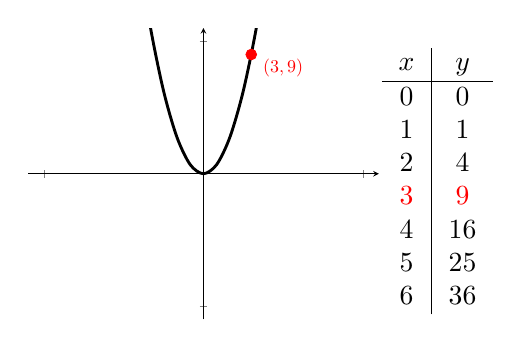
\begin{tikzpicture}[scale=0.65]
    \begin{axis}[
    axis x line=center,
    axis y line=center,
    ytick={-10,10},
    yticklabels={},
    xtick={-10,10},
    xticklabels={},
    xmin=-11, xmax=11, ymin=-11, ymax=11,
    ]
\plot[domain=-10:10, smooth, ultra thick, black]{x^2};
\filldraw[red] (axis cs:3,9) circle(3pt);
\node[red] at (axis cs: 5,8) {$(3,9)$};
\end{axis}
\node[anchor=north] at (8,5.5) {
\begin{tabular}{c|c}
$x$ & $y$ \\\hline
$0 $ & $0 $ \\
$1 $ & $1 $ \\
$2 $ & $4 $ \\
{\color{red}$3$} & ${\color{red}9} $ \\
$4$ & $16 $ \\
$5$ & $25 $ \\
$6$ & $36$ \\
\end{tabular}
};
\end{tikzpicture}
&
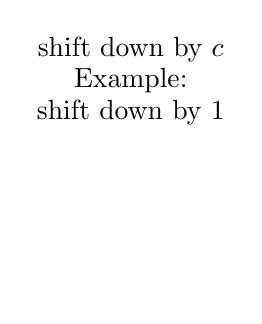
\begin{tikzpicture}
\node at (0,3.0) {shift down by $c$};
\node at (0,2.6) {Example:};
\node at (0,2.2) {shift down by $1$};
\node at (0,0) {\phantom{.}};
\end{tikzpicture}

&
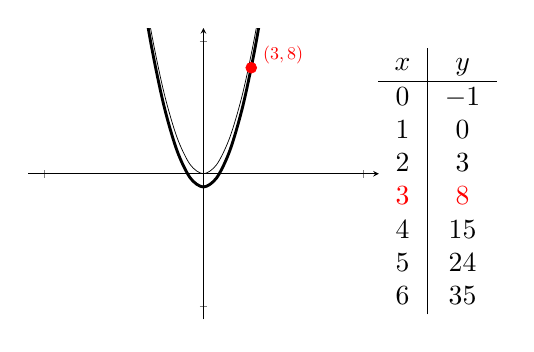
\begin{tikzpicture}[scale=0.65]
    \begin{axis}[
    axis x line=center,
    axis y line=center,
    ytick={-10,10},
    yticklabels={},
    xtick={-10,10},
    xticklabels={},
    xmin=-11, xmax=11, ymin=-11, ymax=11,
    ]
\plot[domain=-10:10, smooth]{x^2};
\plot[domain=-10:10, smooth, ultra thick, black]{x^2-1};
\filldraw[red] (axis cs:3,8) circle(3pt);
\node[red] at (axis cs: 5,9) {$(3,8)$};
\end{axis}
\node[anchor=north] at (8,5.5) {
\begin{tabular}{c|c}
$x$ & $y$ \\\hline
$0 $ & $-1 $ \\
$1 $ & $0 $ \\
$2 $ & $3 $ \\
{\color{red}$3$} & ${\color{red}8} $ \\
$4$ & $15 $ \\
$5$ & $24 $ \\
$6$ & $35$ \\
\end{tabular}
};
\end{tikzpicture}
\\\hline
\end{tabular}
\end{center}


\begin{center}
\begin{tabular}{|c|c|c|c|}\hline
& $y=f(x)$ original &&  $y=c\,f(x)$\\
& Ex: $y=x^2$ original && Ex: $y=2x^2$\\
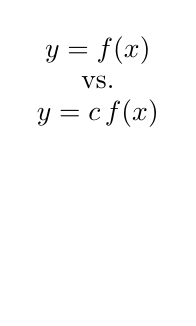
\begin{tikzpicture}
\node at (0,3.0) {$y=f(x)$};
\node at (0,2.6) {vs.};
\node at (0,2.2) {$y=c\,f(x)$};
\node at (0,0) {\phantom{.}};
\end{tikzpicture}
&
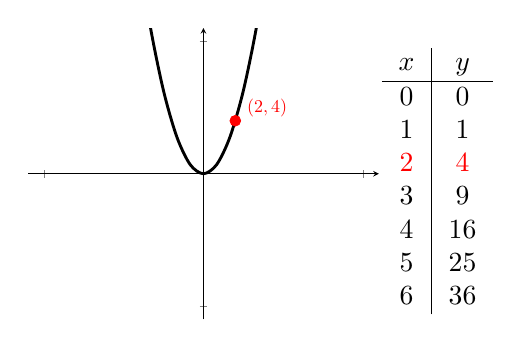
\begin{tikzpicture}[scale=0.65]
    \begin{axis}[
    axis x line=center,
    axis y line=center,
    ytick={-10,10},
    yticklabels={},
    xtick={-10,10},
    xticklabels={},
    xmin=-11, xmax=11, ymin=-11, ymax=11,
    ]
\plot[domain=-10:10, smooth, ultra thick, black]{x^2};
\filldraw[red] (axis cs:2,4) circle(3pt);
\node[red] at (axis cs: 4,5) {$(2,4)$};
\end{axis}
\node[anchor=north] at (8,5.5) {
\begin{tabular}{c|c}
$x$ & $y$ \\\hline
$0 $ & $0 $ \\
$1 $ & $1 $ \\
{\color{red}$2$} & ${\color{red}4} $ \\
$3$ & $9 $ \\
$4$ & $16 $ \\
$5$ & $25 $ \\
$6$ & $36$ \\
\end{tabular}
};
\end{tikzpicture}
&
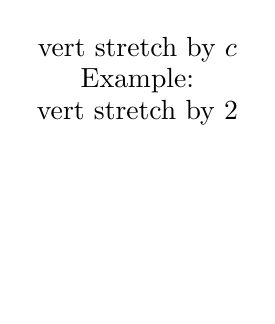
\begin{tikzpicture}
\node at (0,3.0) {vert stretch by $c$};
\node at (0,2.6) {Example:};
\node at (0,2.2) {vert stretch by $2$};
\node at (0,0) {\phantom{.}};
\end{tikzpicture}

&
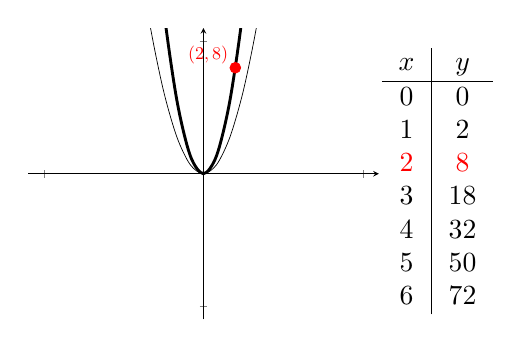
\begin{tikzpicture}[scale=0.65]
    \begin{axis}[
    axis x line=center,
    axis y line=center,
    ytick={-10,10},
    yticklabels={},
    xtick={-10,10},
    xticklabels={},
    xmin=-11, xmax=11, ymin=-11, ymax=11,
    ]
\plot[domain=-10:10, smooth]{x^2};
\plot[domain=-10:10, smooth, ultra thick, black]{2*x^2};
\filldraw[red] (axis cs:2,8) circle(3pt);
\node[red] at (axis cs: .3,9) {$(2,8)$};
\end{axis}
\node[anchor=north] at (8,5.5) {
\begin{tabular}{c|c}
$x$ & $y$ \\\hline
$0 $ & $0 $ \\
$1 $ & $2 $ \\
{\color{red}$2$} & ${\color{red}8} $ \\
$3$ & $18$ \\
$4$ & $32$ \\
$5$ & $50$ \\
$6$ & $72$ \\
\end{tabular}
};
\end{tikzpicture}
\\\hline
\end{tabular}
\end{center}


\begin{center}
\begin{tabular}{|c|c|c|c|}\hline
& $y=f(x)$ original &&  $y=\frac1cf(x)$ \\
& Ex: $y=x^2$ original && Ex: $y=\frac12x^2$\\
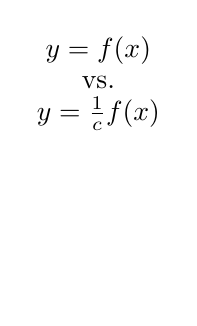
\begin{tikzpicture}
\node at (0,3.0) {$y=f(x)$};
\node at (0,2.6) {vs.};
\node at (0,2.2) {$y=\frac1cf(x)$};
\node at (0,0) {\phantom{.}};
\end{tikzpicture}
&
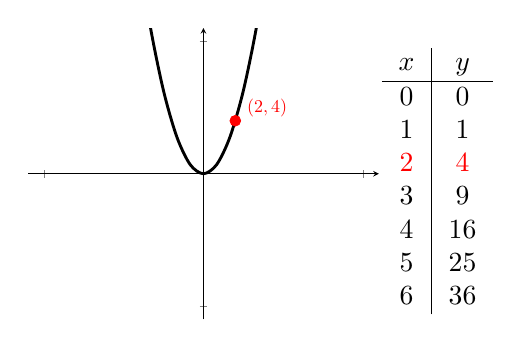
\begin{tikzpicture}[scale=0.65]
    \begin{axis}[
    axis x line=center,
    axis y line=center,
    ytick={-10,10},
    yticklabels={},
    xtick={-10,10},
    xticklabels={},
    xmin=-11, xmax=11, ymin=-11, ymax=11,
    ]
\plot[domain=-10:10, smooth, ultra thick, black]{x^2};
\filldraw[red] (axis cs:2,4) circle(3pt);
\node[red] at (axis cs: 4,5) {$(2,4)$};
\end{axis}
\node[anchor=north] at (8,5.5) {
\begin{tabular}{c|c}
$x$ & $y$ \\\hline
$0 $ & $0 $ \\
$1 $ & $1 $ \\
{\color{red}$2$} & ${\color{red}4} $ \\
$3$ & $9 $ \\
$4$ & $16 $ \\
$5$ & $25 $ \\
$6$ & $36$ \\
\end{tabular}
};
\end{tikzpicture}
&
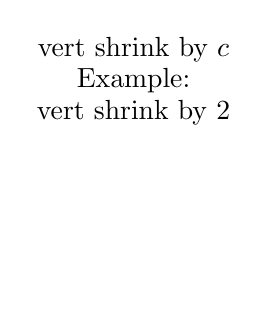
\begin{tikzpicture}
\node at (0,3.0) {vert shrink by $c$};
\node at (0,2.6) {Example:};
\node at (0,2.2) {vert shrink by $2$};
\node at (0,0) {\phantom{.}};
\end{tikzpicture}
&
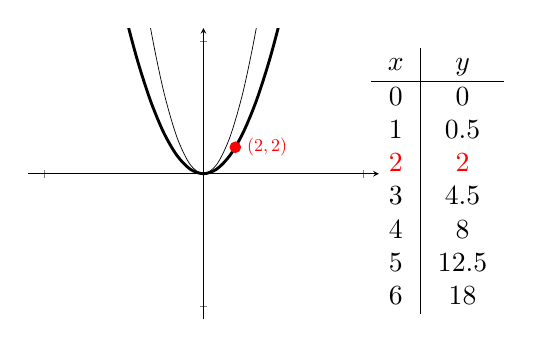
\begin{tikzpicture}[scale=0.65]
    \begin{axis}[
    axis x line=center,
    axis y line=center,
    ytick={-10,10},
    yticklabels={},
    xtick={-10,10},
    xticklabels={},
    xmin=-11, xmax=11, ymin=-11, ymax=11,
    ]
\plot[domain=-10:10, smooth]{x^2};
\plot[domain=-10:10, smooth, ultra thick, black]{x^2/2};
\filldraw[red] (axis cs:2,2) circle(3pt);
\node[red] at (axis cs: 4,2) {$(2,2)$};
\end{axis}
\node[anchor=north] at (8,5.5) {
\begin{tabular}{c|c}
$x$ & $y$ \\\hline
$0 $ & $0 $ \\
$1 $ & $0.5 $ \\
{\color{red}$2$} & ${\color{red}2} $ \\
$3$ & $4.5$ \\
$4$ & $8$ \\
$5$ & $12.5$ \\
$6$ & $18$ \\
\end{tabular}
};
\end{tikzpicture}
\\\hline
\end{tabular}
\end{center}


\begin{center}
\begin{tabular}{|c|c|c|c|}\hline
& $y=f(x)$ original & & $y=-f(x)$\\
& Ex: $y=x^2$ original && Ex: $y=-x^2$ \\
\begin{tikzpicture}
\node at (0,3.0) {$y=f(x)$};
\node at (0,2.6) {vs.};
\node at (0,2.2) {$y=-f(x)$};
\node at (0,0) {\phantom{.}};
\end{tikzpicture}
&
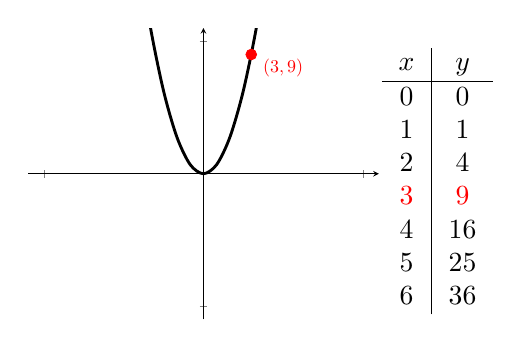
\begin{tikzpicture}[scale=0.65]
    \begin{axis}[
    axis x line=center,
    axis y line=center,
    ytick={-10,10},
    yticklabels={},
    xtick={-10,10},
    xticklabels={},
    xmin=-11, xmax=11, ymin=-11, ymax=11,
    ]
\plot[domain=-10:10, smooth, ultra thick, black]{x^2};
\filldraw[red] (axis cs:3,9) circle(3pt);
\node[red] at (axis cs: 5,8) {$(3,9)$};
\end{axis}
\node[anchor=north] at (8,5.5) {
\begin{tabular}{c|c}
$x$ & $y$ \\\hline
$0 $ & $0 $ \\
$1 $ & $1 $ \\
$2 $ & $4 $ \\
{\color{red}$3$} & ${\color{red}9} $ \\
$4$ & $16 $ \\
$5$ & $25 $ \\
$6$ & $36$ \\
\end{tabular}
};
\end{tikzpicture}
&\begin{tikzpicture}
\node at (0,2.6) {flip vert};
\node at (0,0) {\phantom{.}};
\end{tikzpicture}
&
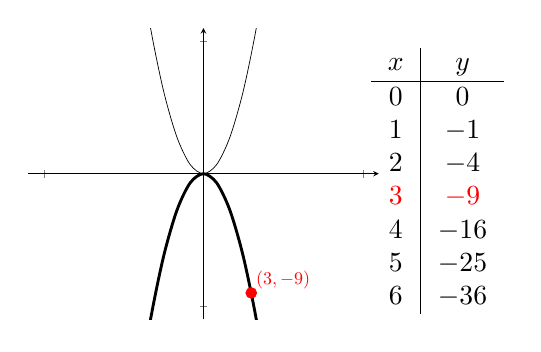
\begin{tikzpicture}[scale=0.65]
    \begin{axis}[
    axis x line=center,
    axis y line=center,
    ytick={-10,10},
    yticklabels={},
    xtick={-10,10},
    xticklabels={},
    xmin=-11, xmax=11, ymin=-11, ymax=11,
    ]
\plot[domain=-10:10, smooth]{x^2};
\plot[domain=-10:10, smooth, ultra thick, black]{-x^2};
\filldraw[red] (axis cs:3,-9) circle(3pt);
\node[red] at (axis cs: 5,-8) {$(3,-9)$};
\end{axis}
\node[anchor=north] at (8,5.5) {
\begin{tabular}{c|c}
$x$ & $y$ \\\hline
$0 $ & $0 $ \\
$1 $ & $-1 $ \\
$2 $ & $-4 $ \\
{\color{red}$3$} & ${\color{red}-9} $ \\
$4$ & $-16 $ \\
$5$ & $-25 $ \\
$6$ & $-36$ \\
\end{tabular}
};
\end{tikzpicture}
\\\hline
\end{tabular}
\end{center}

%\newpage



\noindent {\bf Horizontal transformations}\\Our example uses $f(x)=\sqrt{x}$. Because $(a,b)$ is on the graph of $y=f(x)$ if and only if $f(a)=b$, we get...
\vskip-32pt
\begin{center}
\begin{tabular}{|c|c|c|c|}\hline

& $y=f(x)$ original& &  $y=f(x+c)$\\
& Ex: $y=\sqrt{x}$ original& & Ex: $y=\sqrt{x+3}$ \\
\begin{tikzpicture}
\node at (0,3.0) {$y=f(x)$};
\node at (0,2.6) {vs.};
\node at (0,2.2) {$y=f(x+c)$};
\node at (0,0) {\phantom{.}};
\end{tikzpicture}
&
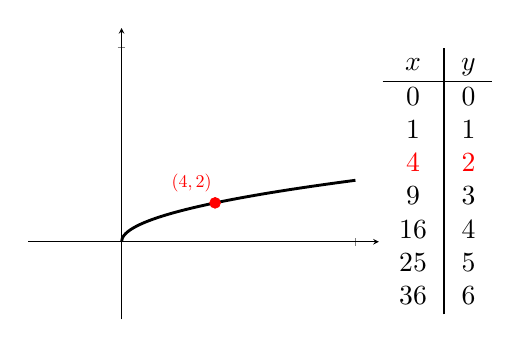
\begin{tikzpicture}[scale=0.65]
    \begin{axis}[
    axis x line=center,
    axis y line=center,
    ytick={-10,10},
    yticklabels={},
    xtick={-10,10},
    xticklabels={},
    xmin=-4, xmax=11, ymin=-4, ymax=11,
    ]
\plot[domain=0:10, smooth, ultra thick, black, samples=300]{sqrt(x)};
\filldraw[red] (axis cs:4,2) circle(3pt);
\node[red] at (axis cs: 3,3) {$(4,2)$};
\end{axis}
\node[anchor=north] at (8,5.5) {
\begin{tabular}{c|c}
$x$ & $y$ \\\hline
$0 $ & $0 $ \\
$1 $ & $1 $ \\
{\color{red}$4$} & ${\color{red}2} $ \\
$9$ & $3 $ \\
$16$ & $4 $ \\
$25$ & $5 $ \\
$36$ & $6$ \\
\end{tabular}
};
\end{tikzpicture}
&
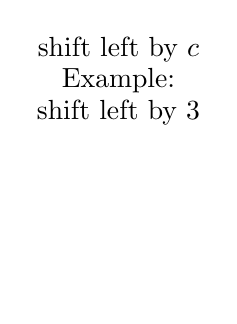
\begin{tikzpicture}
\node at (0,3.0) {shift left by $c$};
\node at (0,2.6) {Example:};
\node at (0,2.2) {shift left by $3$};
\node at (0,0) {\phantom{.}};
\end{tikzpicture}
&

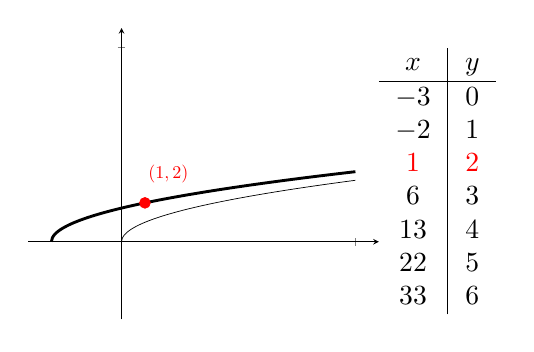
\begin{tikzpicture}[scale=0.65]
    \begin{axis}[
    axis x line=center,
    axis y line=center,
    ytick={-10,10},
    yticklabels={},
    xtick={-10,10},
    xticklabels={},
    xmin=-4, xmax=11, ymin=-4, ymax=11,
    ]
\plot[domain=0:10, smooth, black, samples=300]{sqrt(x)};
\plot[domain=-3:10, smooth, ultra thick, black, samples=300]{sqrt(x+3)};
\filldraw[red] (axis cs:1,2) circle(3pt);
\node[red] at (axis cs: 2,3.5) {$(1,2)$};
\end{axis}
\node[anchor=north] at (8,5.5) {
\begin{tabular}{c|c}
$x$ & $y$ \\\hline
$-3 $ & $0 $ \\
$-2 $ & $1 $ \\
{\color{red}$1$} & ${\color{red}2} $ \\
$6$ & $3 $ \\
$13$ & $4 $ \\
$22$ & $5 $ \\
$33$ & $6$ \\
\end{tabular}
};
\end{tikzpicture}
\\\hline
\end{tabular}
\end{center}


\begin{center}
\begin{tabular}{|c|c|c|c|}\hline
& $y=f(x)$ original &&  $y=f(x-c)$\\
& Ex: $y=\sqrt{x}$ original && Ex: $y=\sqrt{x-3}$ \\
\begin{tikzpicture}
\node at (0,3.0) {$y=f(x)$};
\node at (0,2.6) {vs.};
\node at (0,2.2) {$y=f(x-c)$};
\node at (0,0) {\phantom{.}};
\end{tikzpicture}
&
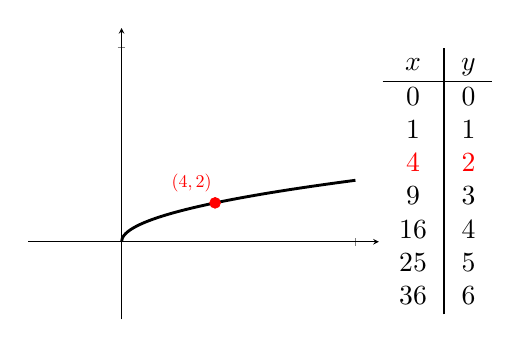
\begin{tikzpicture}[scale=0.65]
    \begin{axis}[
    axis x line=center,
    axis y line=center,
    ytick={-10,10},
    yticklabels={},
    xtick={-10,10},
    xticklabels={},
    xmin=-4, xmax=11, ymin=-4, ymax=11,
    ]
\plot[domain=0:10, smooth, ultra thick, black, samples=300]{sqrt(x)};
\filldraw[red] (axis cs:4,2) circle(3pt);
\node[red] at (axis cs: 3,3) {$(4,2)$};
\end{axis}
\node[anchor=north] at (8,5.5) {
\begin{tabular}{c|c}
$x$ & $y$ \\\hline
$0 $ & $0 $ \\
$1 $ & $1 $ \\
{\color{red}$4$} & ${\color{red}2} $ \\
$9$ & $3 $ \\
$16$ & $4 $ \\
$25$ & $5 $ \\
$36$ & $6$ \\
\end{tabular}

};
\end{tikzpicture}
&
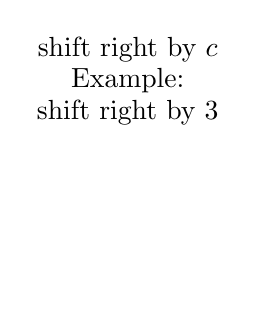
\begin{tikzpicture}
\node at (0,3.0) {shift right by $c$};
\node at (0,2.6) {Example:};
\node at (0,2.2) {shift right by $3$};
\node at (0,0) {\phantom{.}};
\end{tikzpicture}
&

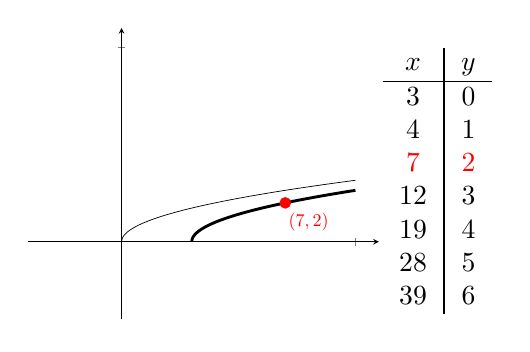
\begin{tikzpicture}[scale=0.65]
    \begin{axis}[
    axis x line=center,
    axis y line=center,
    ytick={-10,10},
    yticklabels={},
    xtick={-10,10},
    xticklabels={},
    xmin=-4, xmax=11, ymin=-4, ymax=11,
    ]
\plot[domain=0:10, smooth, black, samples=300]{sqrt(x)};
\plot[domain=3:10, smooth, ultra thick, black, samples=300]{sqrt(x-3)};
\filldraw[red] (axis cs:7,2) circle(3pt);
\node[red] at (axis cs: 8,1) {$(7,2)$};
\end{axis}
\node[anchor=north] at (8,5.5) {
\begin{tabular}{c|c}
$x$ & $y$ \\\hline
$3 $ & $0 $ \\
$4 $ & $1 $ \\
{\color{red}$7$} & ${\color{red}2} $ \\
$12$ & $3 $ \\
$19$ & $4 $ \\
$28$ & $5 $ \\
$39$ & $6$ \\
\end{tabular}
};
\end{tikzpicture}
\\\hline
\end{tabular}
\end{center}


\begin{center}
\begin{tabular}{|c|c|c|c|}\hline
& $y=f(x)$ original &&  $y=f(cx)$ \\
& Ex: $y=\sqrt{x}$ original && Ex: $y=\sqrt{2x}$ \\
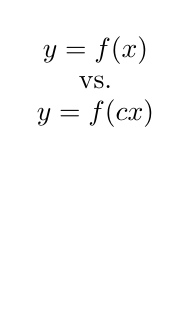
\begin{tikzpicture}
\node at (0,3.0) {$y=f(x)$};
\node at (0,2.6) {vs.};
\node at (0,2.2) {$y=f(cx)$};
\node at (0,0) {\phantom{.}};
\end{tikzpicture}
&
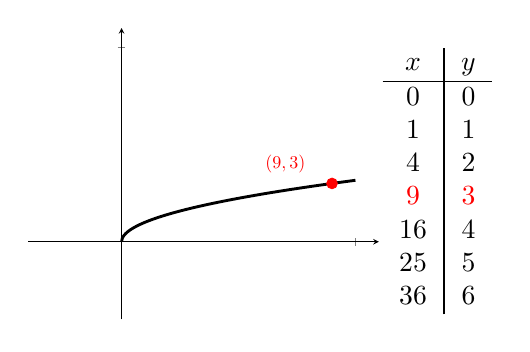
\begin{tikzpicture}[scale=0.65]
    \begin{axis}[
    axis x line=center,
    axis y line=center,
    ytick={-10,10},
    yticklabels={},
    xtick={-10,10},
    xticklabels={},
    xmin=-4, xmax=11, ymin=-4, ymax=11,
    ]
\plot[domain=0:10, smooth, ultra thick, black, samples=300]{sqrt(x)};
\filldraw[red] (axis cs:9,3) circle(3pt);
\node[red] at (axis cs: 7,4) {$(9,3)$};
\end{axis}
\node[anchor=north] at (8,5.5) {
\begin{tabular}{c|c}
$x$ & $y$ \\\hline
$0 $ & $0 $ \\
$1 $ & $1 $ \\
$4 $ & $2 $ \\
{\color{red}$9$} & ${\color{red}3} $ \\
$16$ & $4 $ \\
$25$ & $5 $ \\
$36$ & $6$ \\
\end{tabular}
};
\end{tikzpicture}
&
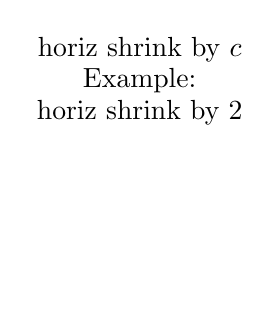
\begin{tikzpicture}
\node at (0,3.0) {horiz shrink by $c$};
\node at (0,2.6) {Example:};
\node at (0,2.2) {horiz shrink by $2$};
\node at (0,0) {\phantom{.}};
\end{tikzpicture}
&

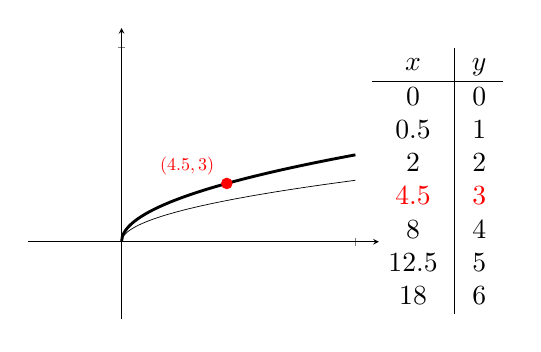
\begin{tikzpicture}[scale=0.65]
    \begin{axis}[
    axis x line=center,
    axis y line=center,
    ytick={-10,10},
    yticklabels={},
    xtick={-10,10},
    xticklabels={},
    xmin=-4, xmax=11, ymin=-4, ymax=11,
    ]
\plot[domain=0:10, smooth, black, samples=300]{sqrt(x)};
\plot[domain=0:10, smooth, ultra thick, black, samples=300]{sqrt(2*x)};
\filldraw[red] (axis cs:4.5,3) circle(3pt);
\node[red] at (axis cs: 2.8,3.9) {$(4.5,3)$};
\end{axis}
\node[anchor=north] at (8,5.5) {
\begin{tabular}{c|c}
$x$ & $y$ \\\hline
$0 $ & $0 $ \\
$0.5 $ & $1 $ \\
$2 $ & $2 $ \\
{\color{red}$4.5$} & ${\color{red}3} $ \\
$8$ & $4 $ \\
$12.5$ & $5 $ \\
$18$ & $6$ \\
\end{tabular}
};
\end{tikzpicture}
\\\hline
\end{tabular}
\end{center}


\begin{center}
\begin{tabular}{|c|c|c|c|}\hline
& $y=f(x)$ original &&  $y=f(\frac1cx)$\\
& Ex: $y=\sqrt{x}$ original && Ex: $y=\sqrt{\frac12x}$ \\
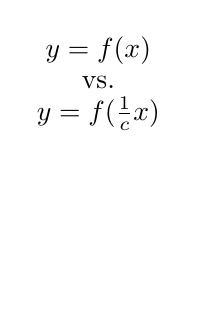
\begin{tikzpicture}
\node at (0,3.0) {$y=f(x)$};
\node at (0,2.6) {vs.};
\node at (0,2.2) {$y=f(\frac1c x)$};
\node at (0,0) {\phantom{.}};
\end{tikzpicture}
&
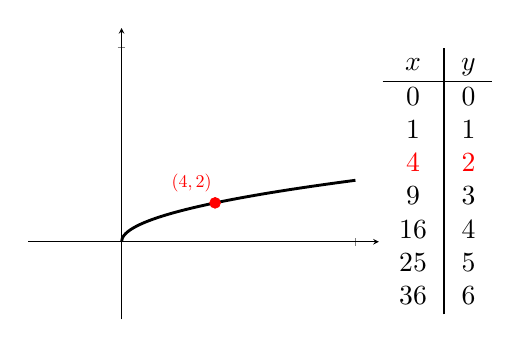
\begin{tikzpicture}[scale=0.65]
    \begin{axis}[
    axis x line=center,
    axis y line=center,
    ytick={-10,10},
    yticklabels={},
    xtick={-10,10},
    xticklabels={},
    xmin=-4, xmax=11, ymin=-4, ymax=11,
    ]
\plot[domain=0:10, smooth, ultra thick, black, samples=300]{sqrt(x)};
\filldraw[red] (axis cs:4,2) circle(3pt);
\node[red] at (axis cs: 3,3) {$(4,2)$};
\end{axis}
\node[anchor=north] at (8,5.5) {
\begin{tabular}{c|c}
$x$ & $y$ \\\hline
$0 $ & $0 $ \\
$1 $ & $1 $ \\
{\color{red}$4$} & ${\color{red}2} $ \\
$9$ & $3 $ \\
$16$ & $4 $ \\
$25$ & $5 $ \\
$36$ & $6$ \\
\end{tabular}
};
\end{tikzpicture}
&
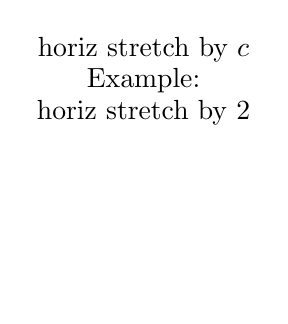
\begin{tikzpicture}
\node at (0,3.0) {horiz stretch by $c$};
\node at (0,2.6) {Example:};
\node at (0,2.2) {horiz stretch by $2$};
\node at (0,0) {\phantom{.}};
\end{tikzpicture}
&

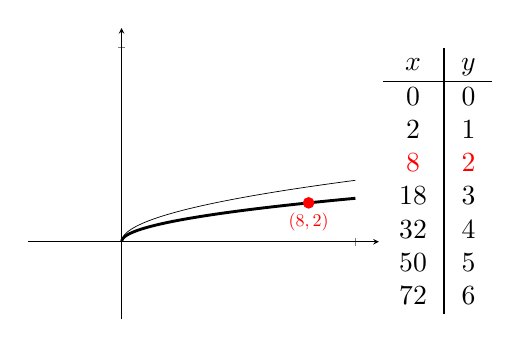
\begin{tikzpicture}[scale=0.65]
    \begin{axis}[
    axis x line=center,
    axis y line=center,
    ytick={-10,10},
    yticklabels={},
    xtick={-10,10},
    xticklabels={},
    xmin=-4, xmax=11, ymin=-4, ymax=11,
    ]
\plot[domain=0:10, smooth, black, samples=300]{sqrt(x)};
\plot[domain=0:10, smooth, ultra thick, black, samples=300]{sqrt(x/2)};
\filldraw[red] (axis cs:8,2) circle(3pt);
\node[red] at (axis cs: 8,1) {$(8,2)$};
\end{axis}
\node[anchor=north] at (8,5.5) {
\begin{tabular}{c|c}
$x$ & $y$ \\\hline
$0 $ & $0 $ \\
$2 $ & $1 $ \\
{\color{red}$8$} & ${\color{red}2} $ \\
$18$ & $3 $ \\
$32$ & $4 $ \\
$50$ & $5 $ \\
$72$ & $6$ \\
\end{tabular}
};
\end{tikzpicture}
\\\hline
\end{tabular}
\end{center}


\begin{center}
\begin{tabular}{|c|c|c|c|}\hline
& $y=f(x)$ original &&  $y=f(-x)$\\
& Ex: $y=\sqrt{x}$ original && Ex: $y=\sqrt{-x}$\\
\begin{tikzpicture}
\node at (0,3.0) {$y=f(x)$};
\node at (0,2.6) {vs.};
\node at (0,2.2) {$y=f(-x)$};
\node at (0,0) {\phantom{.}};
\end{tikzpicture}
&
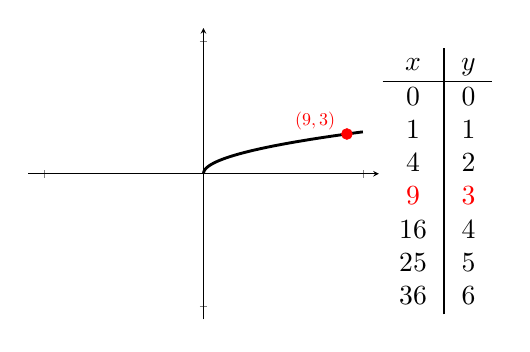
\begin{tikzpicture}[scale=0.65]
    \begin{axis}[
    axis x line=center,
    axis y line=center,
    ytick={-10,10},
    yticklabels={},
    xtick={-10,10},
    xticklabels={},
    xmin=-11, xmax=11, ymin=-11, ymax=11,
    ]
\plot[domain=0:10, smooth, ultra thick, black, samples=300]{sqrt(x)};
\filldraw[red] (axis cs:9,3) circle(3pt);
\node[red] at (axis cs: 7,4) {$(9,3)$};
\end{axis}
\node[anchor=north] at (8,5.5) {
\begin{tabular}{c|c}
$x$ & $y$ \\\hline
$0 $ & $0 $ \\
$1 $ & $1 $ \\
$4 $ & $2 $ \\
{\color{red}$9$} & ${\color{red}3} $ \\
$16$ & $4 $ \\
$25$ & $5 $ \\
$36$ & $6$ \\
\end{tabular}
};
\end{tikzpicture}
&
\begin{tikzpicture}
\node at (0,2.6) {flip horiz};
\node at (0,0) {\phantom{.}};
\end{tikzpicture}
&

\begin{tikzpicture}[scale=0.65]
    \begin{axis}[
    axis x line=center,
    axis y line=center,
    ytick={-10,10},
    yticklabels={},
    xtick={-10,10},
    xticklabels={},
    xmin=-11, xmax=11, ymin=-11, ymax=11,
    ]
\plot[domain=0:10, smooth, black, samples=300]{sqrt(x)};
\plot[domain=-10:0, smooth, ultra thick, black, samples=300]{sqrt(-x)};
\filldraw[red] (axis cs:-9,3) circle(3pt);
\node[red] at (axis cs: -7,4) {$(-9,3)$};
\end{axis}
\node[anchor=north] at (8,5.5) {
\begin{tabular}{c|c}
$x$ & $y$ \\\hline
$0 $ & $0 $ \\
$-1 $ & $1 $ \\
$-4 $ & $2 $ \\
{\color{red}$-9$} & ${\color{red}3} $ \\
$-16$ & $4 $ \\
$-25$ & $5 $ \\
$-36$ & $6$ \\
\end{tabular}
};
\end{tikzpicture}
\\\hline
\end{tabular}
\end{center}




%\newpage


\begin{tikzpicture}[scale=0.4]
\draw[step=1cm,gray,very thin] (-6.5,-6.5) grid (6.5,6.5);
\draw[thick, ->] (-6.5,0) -- (7,0);
\draw[thick, ->] (0,-6.5) -- (0,7);
\node at (0,-7.2) {Graph of $y=f(x)$};
\node at (6.5,.5) {$x$};
\node at (.5,6.5) {$y$};
\node at (5,-.5) {$5$};
\node at (-.5,5) {$5$};
\draw[thick, <->] (-5,-6) -- (-1,2) -- (3,-2) -- (6,4);
\end{tikzpicture}
\qquad\qquad
\begin{tikzpicture}[scale=0.4]
\draw[step=1cm,gray,very thin] (-6.5,-6.5) grid (6.5,6.5);
\draw[thick, ->] (-6.5,0) -- (7,0);
\draw[thick, ->] (0,-6.5) -- (0,7);
\node at (0,-7.2) {Graph of $y=f(x)+3$};
\node at (6.5,.5) {$x$};
\node at (.5,6.5) {$y$};
\node at (5,-.5) {$5$};
\node at (-.5,5) {$5$};
\end{tikzpicture}
\qquad\qquad
\begin{tikzpicture}[scale=0.4]
\draw[white] (-2,-6.5) -- (2,7);
\node at (0,6) {Based on the ``original function''};
\node at (0,5) {on the left, sketch the graph};
\node at (0,4) {of the graph transformation};

\node at (0,2.5) {Carefully determine if the};
\node at (0,1.5) {transformation is vertical};
\node at (0,.5) {or horizontal};
\end{tikzpicture}


\vskip10pt

\begin{tikzpicture}[scale=0.4]
\draw[step=1cm,gray,very thin] (-6.5,-6.5) grid (6.5,6.5);
\draw[thick, ->] (-6.5,0) -- (7,0);
\draw[thick, ->] (0,-6.5) -- (0,7);
\node at (0,-7.2) {Graph of $y=g(x)$};
\node at (6.5,.5) {$x$};
\node at (.5,6.5) {$y$};
\node at (5,-.5) {$5$};
\node at (-.5,5) {$5$};
\draw[thick, <->] (-6,-6) -- (-3,2) -- (3,4) -- (6,1);
\end{tikzpicture}
\qquad\qquad
\begin{tikzpicture}[scale=0.4]
\draw[step=1cm,gray,very thin] (-6.5,-6.5) grid (6.5,6.5);
\draw[thick, ->] (-6.5,0) -- (7,0);
\draw[thick, ->] (0,-6.5) -- (0,7);
\node at (0,-7.2) {Graph of $y=g(x+3)$};
\node at (6.5,.5) {$x$};
\node at (.5,6.5) {$y$};
\node at (5,-.5) {$5$};
\node at (-.5,5) {$5$};
\end{tikzpicture}
\qquad\qquad
\begin{tikzpicture}
\end{tikzpicture}



\vskip10pt



\begin{tikzpicture}[scale=0.4]
\draw[step=1cm,gray,very thin] (-6.5,-6.5) grid (6.5,6.5);
\draw[thick, ->] (-6.5,0) -- (7,0);
\draw[thick, ->] (0,-6.5) -- (0,7);
\node at (0,-7.2) {Graph of $y=h(x)$};
\node at (6.5,.5) {$x$};
\node at (.5,6.5) {$y$};
\node at (5,-.5) {$5$};
\node at (-.5,5) {$5$};
\draw[thick, <->] (-6,-3) -- (-4,3) -- (-2,-3) -- (0,3) -- (2,-3) -- (4,3) -- (6,-3);
\end{tikzpicture}
\qquad\qquad
\begin{tikzpicture}[scale=0.4]
\draw[step=1cm,gray,very thin] (-6.5,-6.5) grid (6.5,6.5);
\draw[thick, ->] (-6.5,0) -- (7,0);
\draw[thick, ->] (0,-6.5) -- (0,7);
\node at (0,-7.2) {Graph of $y=2\,h(x)$};
\node at (6.5,.5) {$x$};
\node at (.5,6.5) {$y$};
\node at (5,-.5) {$5$};
\node at (-.5,5) {$5$};
\end{tikzpicture}
\qquad\qquad
\begin{tikzpicture}
\end{tikzpicture}




\vskip10pt



\begin{tikzpicture}[scale=0.4]
\draw[step=1cm,gray,very thin] (-6.5,-6.5) grid (6.5,6.5);
\draw[thick, ->] (-6.5,0) -- (7,0);
\draw[thick, ->] (0,-6.5) -- (0,7);
\node at (0,-7.2) {Graph of $y=k(x)$};
\node at (6.5,.5) {$x$};
\node at (.5,6.5) {$y$};
\node at (5,-.5) {$5$};
\node at (-.5,5) {$5$};
\draw[thick, <->] (-6,4) -- (-4,2) -- (2,2) -- (4,5) -- (6,-3);
\end{tikzpicture}
\qquad\qquad
\begin{tikzpicture}[scale=0.4]
\draw[step=1cm,gray,very thin] (-6.5,-6.5) grid (6.5,6.5);
\draw[thick, ->] (-6.5,0) -- (7,0);
\draw[thick, ->] (0,-6.5) -- (0,7);
\node at (0,-7.2) {Graph of $y=k(2x)$};
\node at (6.5,.5) {$x$};
\node at (.5,6.5) {$y$};
\node at (5,-.5) {$5$};
\node at (-.5,5) {$5$};
\end{tikzpicture}
\qquad\qquad
\begin{tikzpicture}[scale=0.4]
\draw[white] (-2,-6.5) -- (2,7);
\node at (0,1) {The suggested order:};
\node at (0,0) {1st, horiz stretch/shrink};
\node at (0,-1) {2nd, horiz shift};
\node at (0,-2) {3rd, vert stretch/shrink};
\node at (0,-3) {4th, vert shift};
\end{tikzpicture}


%\newpage

\fbox{
\begin{tikzpicture}[scale=0.35]
\draw[step=1cm,gray,very thin] (-6.5,-6.5) grid (6.5,6.5);
\draw[thick, ->] (-6.5,0) -- (7,0);
\draw[thick, ->] (0,-6.5) -- (0,7);
\node at (0,-7.2) {Graph of $y=f(x)$};
\node at (6.5,.5) {$x$};
\node at (.5,6.5) {$y$};
\node at (5,-.5) {$5$};
\node at (-.5,5) {$5$};
\draw[thick, <->] (-6,5) -- (-3,2) -- (-2,3) -- (2,-1) -- (5.5,6);
\end{tikzpicture}
\qquad\qquad
\begin{tikzpicture}[scale=0.35]
\draw[step=1cm,gray,very thin] (-6.5,-6.5) grid (6.5,6.5);
\draw[thick, ->] (-6.5,0) -- (7,0);
\draw[thick, ->] (0,-6.5) -- (0,7);
\node at (0,-7.2) {Graph of $y=f(x-2)$};
\node at (6.5,.5) {$x$};
\node at (.5,6.5) {$y$};
\node at (5,-.5) {$5$};
\node at (-.5,5) {$5$};
\end{tikzpicture}
\qquad\qquad
\begin{tikzpicture}[scale=0.35]
\draw[step=1cm,gray,very thin] (-6.5,-6.5) grid (6.5,6.5);
\draw[thick, ->] (-6.5,0) -- (7,0);
\draw[thick, ->] (0,-6.5) -- (0,7);
\node at (0,-7.2) {Graph of $y=f(x-2)-3$};
\node at (6.5,.5) {$x$};
\node at (.5,6.5) {$y$};
\node at (5,-.5) {$5$};
\node at (-.5,5) {$5$};
\end{tikzpicture}
}

\vskip10pt


\fbox{
\begin{tikzpicture}[scale=0.35]
\draw[step=1cm,gray,very thin] (-6.5,-6.5) grid (6.5,6.5);
\draw[thick, ->] (-6.5,0) -- (7,0);
\draw[thick, ->] (0,-6.5) -- (0,7);
\node at (0,-7.2) {Graph of $y=g(x)$};
\node at (6.5,.5) {$x$};
\node at (.5,6.5) {$y$};
\node at (5,-.5) {$5$};
\node at (-.5,5) {$5$};
\draw[thick, <->] (-6,-4) -- (-2,2) -- (4,-4) -- (6,-1);
\end{tikzpicture}
\qquad\qquad
\begin{tikzpicture}[scale=0.35]
\draw[step=1cm,gray,very thin] (-6.5,-6.5) grid (6.5,6.5);
\draw[thick, ->] (-6.5,0) -- (7,0);
\draw[thick, ->] (0,-6.5) -- (0,7);
\node at (0,-7.2) {Graph of $y=g(2x)$};
\node at (6.5,.5) {$x$};
\node at (.5,6.5) {$y$};
\node at (5,-.5) {$5$};
\node at (-.5,5) {$5$};
\end{tikzpicture}
\qquad\qquad
\begin{tikzpicture}[scale=0.35]
\draw[step=1cm,gray,very thin] (-6.5,-6.5) grid (6.5,6.5);
\draw[thick, ->] (-6.5,0) -- (7,0);
\draw[thick, ->] (0,-6.5) -- (0,7);
\node at (0,-7.2) {Graph of $y=g(2x)+1$};
\node at (6.5,.5) {$x$};
\node at (.5,6.5) {$y$};
\node at (5,-.5) {$5$};
\node at (-.5,5) {$5$};
\end{tikzpicture}
}

\vskip10pt

%\newpage

\fbox{
\begin{tikzpicture}[scale=0.35]
\draw[step=1cm,gray,very thin] (-6.5,-6.5) grid (6.5,6.5);
\draw[thick, ->] (-6.5,0) -- (7,0);
\draw[thick, ->] (0,-6.5) -- (0,7);
\node at (0,-7.2) {Graph of $y=h(x)$};
\node at (6.5,.5) {$x$};
\node at (.5,6.5) {$y$};
\node at (5,-.5) {$5$};
\node at (-.5,5) {$5$};
\draw[thick, <->] (-6,-5) -- (-2,-5) -- (2,2) -- (6,4);
\end{tikzpicture}
\qquad\qquad
\begin{tikzpicture}[scale=0.35]
\draw[step=1cm,gray,very thin] (-6.5,-6.5) grid (6.5,6.5);
\draw[thick, ->] (-6.5,0) -- (7,0);
\draw[thick, ->] (0,-6.5) -- (0,7);
\node at (0,-7.2) {Graph of $y=h(x+3)$};
\node at (6.5,.5) {$x$};
\node at (.5,6.5) {$y$};
\node at (5,-.5) {$5$};
\node at (-.5,5) {$5$};
\end{tikzpicture}
\qquad\qquad
\begin{tikzpicture}[scale=0.35]
\draw[step=1cm,gray,very thin] (-6.5,-6.5) grid (6.5,6.5);
\draw[thick, ->] (-6.5,0) -- (7,0);
\draw[thick, ->] (0,-6.5) -- (0,7);
\node at (0,-7.2) {Graph of $y=-\,h(x+3)$};
\node at (6.5,.5) {$x$};
\node at (.5,6.5) {$y$};
\node at (5,-.5) {$5$};
\node at (-.5,5) {$5$};
\end{tikzpicture}
}

\vskip10pt


% Precursor to $y = 3 \cos(x) -1$
\fbox{
\begin{tikzpicture}[scale=0.35]
\draw[step=1cm,gray,very thin] (-6.5,-6.5) grid (6.5,6.5);
\draw[thick, ->] (-6.5,0) -- (7,0);
\draw[thick, ->] (0,-6.5) -- (0,7);
\node at (0,-7.2) {Graph of $y=k(x)$};
\node at (6.5,.5) {$x$};
\node at (.5,6.5) {$y$};
\node at (5,-.5) {$5$};
\node at (-.5,5) {$5$};
\draw[thick, <->] (-6,-1) -- (-4,1) -- (-2,-1) -- (0,1) -- (2,-1) -- (4,1) -- (6,-1);
\end{tikzpicture}
\qquad\qquad
\begin{tikzpicture}[scale=0.35]
\draw[step=1cm,gray,very thin] (-6.5,-6.5) grid (6.5,6.5);
\draw[thick, ->] (-6.5,0) -- (7,0);
\draw[thick, ->] (0,-6.5) -- (0,7);
\node at (0,-7.2) {Graph of $y=3\, k(x)$};
\node at (6.5,.5) {$x$};
\node at (.5,6.5) {$y$};
\node at (5,-.5) {$5$};
\node at (-.5,5) {$5$};
\end{tikzpicture}
\qquad\qquad
\begin{tikzpicture}[scale=0.35]
\draw[step=1cm,gray,very thin] (-6.5,-6.5) grid (6.5,6.5);
\draw[thick, ->] (-6.5,0) -- (7,0);
\draw[thick, ->] (0,-6.5) -- (0,7);
\node at (0,-7.2) {Graph of $y=3\,k(x)-1$};
\node at (6.5,.5) {$x$};
\node at (.5,6.5) {$y$};
\node at (5,-.5) {$5$};
\node at (-.5,5) {$5$};
\end{tikzpicture}
}

\vskip10pt

%\newpage


\section{Base Graphs}
\subsection{$f(x)=x$}
\begin{center}
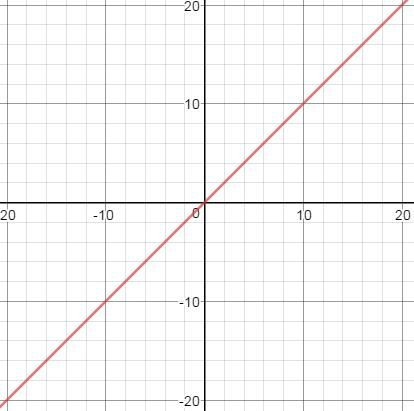
\includegraphics[scale=.4]{line.JPG}
\end{center}
\begin{itemize}
	\item  Domain: $(-\infty, \infty)$   
	\item  Range: $(-\infty, \infty)$ 
		\item $x$-intercepts: $(0,0)$ 
				\item $y$-intercepts: $(0,0)$  
\end{itemize}	


\subsection{$f(x)=x^2$}

\begin{center}
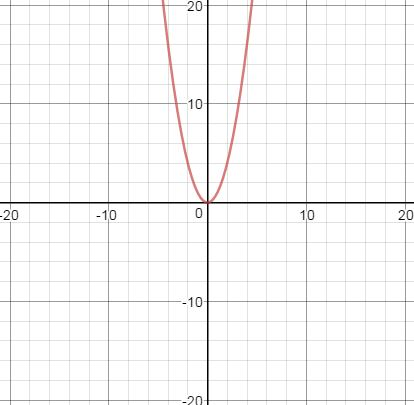
\includegraphics[scale=.4]{quad.JPG}
\end{center}

\begin{itemize}
	\item  Domain:  $(-\infty, \infty)$ 
	\item  Range: $[0,\infty)$
		\item $x$-intercepts: $(0,0)$
				\item $y$-intercepts: $(0,0)$ 
\end{itemize}	


\subsection{$f(x)=x^3$}

\begin{center}
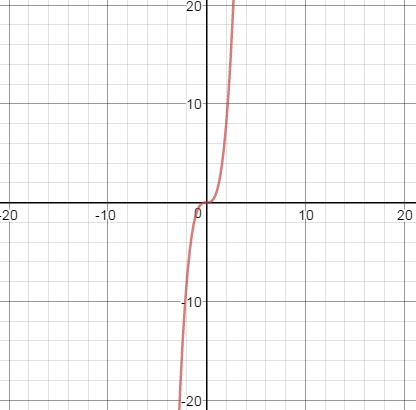
\includegraphics[scale=.4]{cubic.JPG}
\end{center}

\begin{itemize}
	\item  Domain: $(-\infty, \infty)$
	\item  Range: $(-\infty, \infty)$ 
		\item $x$-intercepts: $(0,0)$ 
				\item $y$-intercepts: $(0,0)$ 
\end{itemize}	


\subsection{$f(x)=\sqrt{x}$}

\begin{center}
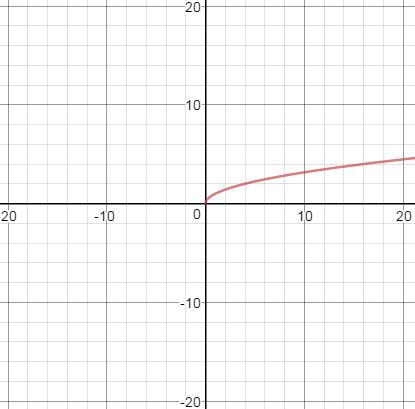
\includegraphics[scale=.4]{squareroot.JPG}
\end{center}

\begin{itemize}
	\item  Domain:  $[0,\infty)$ 
	\item  Range: $[0, \infty)$ 
		\item $x$-intercepts: $(0,0)$ 
				\item $y$-intercepts: $(0,0)$
\end{itemize}	


\subsection{$f(x)=\sqrt[3]{x}$}

\begin{center}
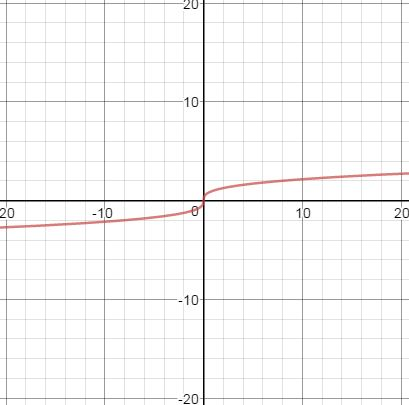
\includegraphics[scale=.4]{cuberoot.JPG}
\end{center}



\begin{itemize}
	\item  Domain: $(-\infty, \infty)$   
	\item  Range: $(-\infty, \infty)$
		\item $x$-intercepts: $(0,0)$
				\item $y$-intercepts: $(0,0)$ 
\end{itemize}	


\subsection{$f(x)=\frac{1}{x}$}

\begin{center}
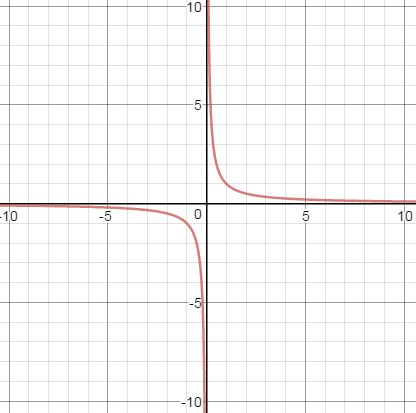
\includegraphics[scale=.4]{1overx.JPG}
\end{center}

\begin{itemize}
	\item  Domain: $(-\infty, 0)\cup(0, \infty)$   
	\item  Range: $(-\infty, 0)\cup(0, \infty)$ 
		\item $x$-intercepts: None
				\item $y$-intercepts:None  
\end{itemize}	


\subsection{$f(x)=\frac{1}{x^2}$}

\begin{center}
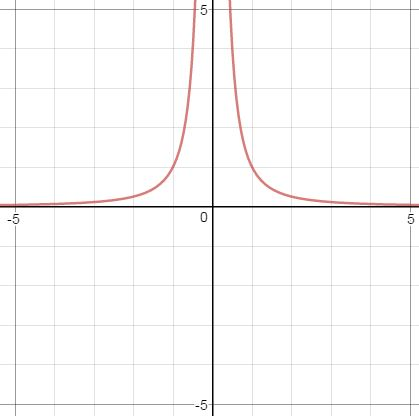
\includegraphics[scale=.4]{1overx2.JPG}
\end{center}

\begin{itemize}
	\item  Domain: $(-\infty, 0)\cup(0, \infty)$   
	\item  Range: $(0,\infty)$
		\item $x$-intercepts: None 
				\item $y$-intercepts: None
\end{itemize}	


\subsection{$f(x)=|x|$}

\begin{center}
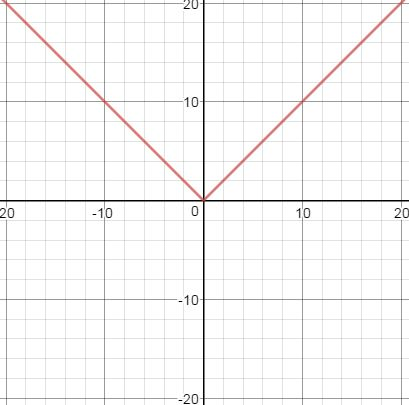
\includegraphics[scale=.4]{absolutevaluex.JPG}
\end{center}

\begin{itemize}
	\item  Domain:$(-\infty, \infty)$    
	\item  Range: $[0,\infty)$ 
		\item $x$-intercepts: $(0,0)$ 
				\item $y$-intercepts: $(0,0)$ 
\end{itemize}	



\section{Transformations of Base Graphs}
 There are several types of graph transformations:  Vertical shifts, horizontal shifts, reflections across the $x$-axis, reflections across the $y$-axis, vertical stretching, and horizontal stretching.


\subsection{Vertical Shifts}

Given a function $f(x)$, the graph of $f(x)+c$ ($c>0$) is the graph of $f(x)$ shifted {\it up} $c$ units.

Given a function $f(x)$, the graph of $f(x)-c$ ($c>0$) is the graph of $f(x)$ shifted {\it down} $c$ units.

\everymath{\displaystyle}
\begin{exm}{Sketch the graph of $g(x)=x^2+3$}
\end{exm}\vskip10pt

\begin{exm}{Sketch the graph of $h(x)=\sqrt{x}-2$}
\end{exm}\vskip10pt



%\newpage
\subsection{Horizontal Shifts}
Given a function $f(x)$, the graph of $f(x+c)$ ($c>0$) is the graph of $f(x)$ shifted {\it left} $c$ units.

Given a function $f(x)$, the graph of $f(x-c)$ ($c>0$) is the graph of $f(x)$ shifted {\it right} $c$ units.

\begin{exm}{Sketch the graph of $f(x)=\frac{1}{x+2}$}
\end{exm}\vskip10pt

\begin{exm}{Sketch the graph of $y=\frac{1}{(x-3)^2}$}
\end{exm}\vskip10pt



\subsection{Reflections}
Given a function $f(x)$, the graph of $-f(x)$ is the graph of $f(x)$ reflected across the {\it $x$-axis}.

Given a function $f(x)$, the graph of $f(-x)$ is the graph of $f(x)$ reflected across the {\it $y$-axis}.

\begin{exm}{Sketch the graph of $f(x)=|-x|$}
\end{exm}\vskip10pt

\begin{exm}{Sketch the graph of $f(x)=-|x|$}
\end{exm}\vskip10pt



%\newpage
\subsection{Vertical Stretching}
Given a function $f(x)$, the graph of $cf(x)$ ($c>1$) is the graph of $f(x)$ stretched vertically by a factor of $c$.

Given a function $f(x)$, the graph of $cf(x)$ ($0<c<1$) is the graph of $f(x)$ compressed vertically by a factor of $\frac{1}{c}$.

  \begin{exm}{Sketch the graph of $f(x)=2x^2+4x+2$}
\end{exm}\vskip10pt

\begin{exm}{Sketch the graph of $g(x)=\frac{1}{2}\left( x-1 \right)^2$}
\end{exm}\vskip10pt



\subsection{Horizontal Stretching}
Given a function $f(x)$, the graph of $f(cx)$ ($c>1$) is the graph of $f(x)$ compressed horizontally by a factor of $c$.

Given a function $f(x)$, the graph of $f(cx)$ ($0<c<1$) is the graph of $f(x)$ stretched horizontally by a factor of $\frac{1}{c}$.

 \begin{exm}{Sketch the graph of $y=\sqrt[3]{8x}$}
\end{exm}\vskip10pt

\begin{exm}{Sketch the graph of $g(x)=\frac{1}{3x}$}
\end{exm}\vskip10pt

%\newpage
\begin{exm}{Graph the function $f(x)=-2(x-4)+3$.}
\end{exm}\vskip10pt

\begin{exm}{If $P(2,-4)$ is on the graph of $f(x)$, what is the corresponding point on the graph of $g(x)=-f(2x)+3$?}
\end{exm}\vskip10pt

\begin{exm}{Below is the graph of $f(x)$. Graph $g(x)=-f(x+1)+3$.  		\begin{center}
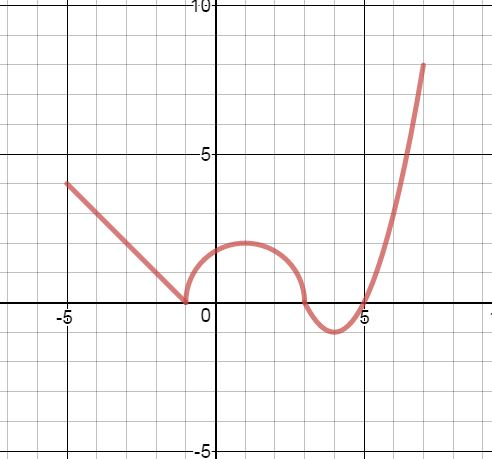
\includegraphics[scale=.3]{trans1.JPG}
\end{center}}
\end{exm}\vskip10pt


%\newpage
\subsection{Even and Odd Functions}
A function is called {\bf even} if $$f(x)=f(-x).$$ Graphically, a function is even if it is symmetric about the $y$-axis. 

A function is called {\bf odd} if $$-f(x)=f(-x).$$ Graphically, a function is even if it is symmetric about the origin. 

\begin{exm}{Give two functions which are even. Then, sketch their graphs.Verify your two functions are even by showing that $f(x)=f(-x)$.}
\end{exm}\vskip10pt


\begin{exm}{Give two functions which are odd. Then, sketch their graphs. Verify your two functions are odd by showing that $-f(x)=f(-x)$.}
\end{exm}\vskip10pt


%\newpage
\section{Piece-wise Functions}
\ A {\bf Piece-wise} defined function is a function which is defined in pieces. For example:
	
$f(x)=\left\{\begin{array}{ll}
|x-3|, &0\leq x<5\\
\frac{1}{2}x^2-10, &5\leq x\leq 6\\
1,& 6<x\leq 8\\
\sqrt{x+1}+3&, x>8\\
\end{array}\right.$   

This looks like the following:

\begin{center}
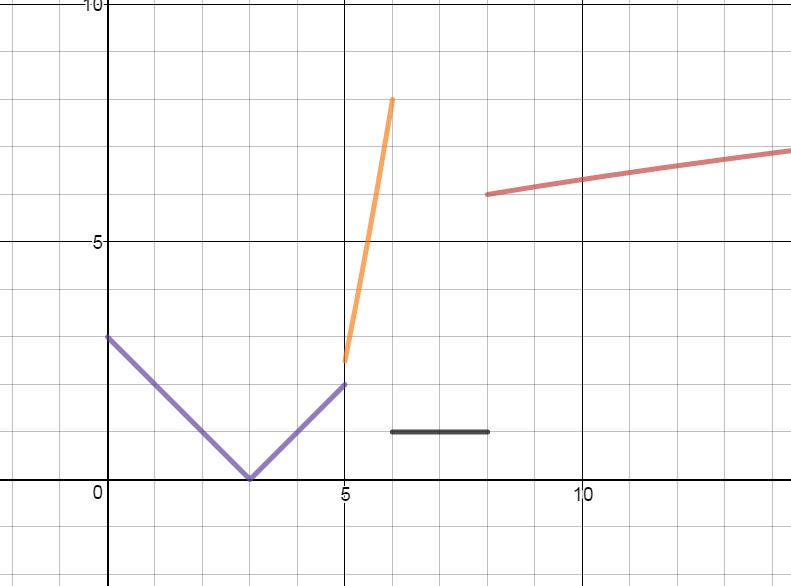
\includegraphics[scale=.3]{piecewise.JPG}
\end{center}

\begin{exm}{For the function, 

	$f(x)=\left\{\begin{array}{ll}
|x-3|, &0\leq x<5\\
\frac{1}{2}x^2-10, &5< x\leq 6\\
1,& 6<x\leq 8\\
\sqrt{x+1}+3&, x>8\\
\end{array}\right.$   
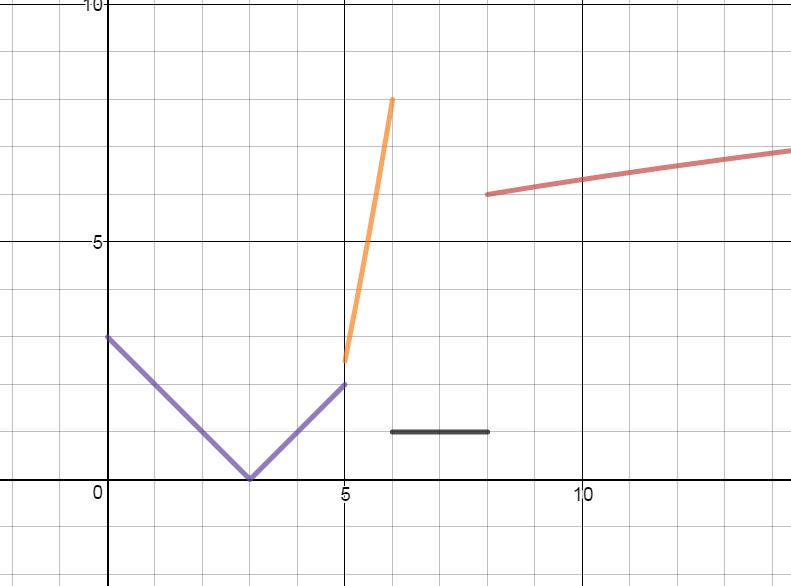
\includegraphics[scale=.2]{piecewise.JPG} 
\begin{itemize}
	\item What is the domain of this function?
	\item What is the range of this function? 
		\item  What is $f(0), ~f(1), ~f(5), ~f(20)$? 
	\item Sketch the graph of $g(x)=-f(-x)$. Then, find the rule for $g(x)$.\end{itemize}}\end{exm}\vskip10pt
	







%\newpage
\renewcommand{\booksection}{Function operations}
\renewcommand{\pageheader}{\booksection }
\section*{\LARGE \pageheader}
%\begin{concepts}
%\item Adding functions
%\item Subtracting functions
%\item Multiplyng functions
%\item Dividing functions
%\item Composition of functions
%\end{concepts}

\begin{bformula}{}{}
$(f+g)(x) = f(x)+g(x)$
\end{bformula}
\begin{bformula}{}{}
$(f-g)(x) = f(x)-g(x)$
\end{bformula}
\begin{bformula}{}{}
$(fg)(x) = f(x) \cdot g(x)$
\end{bformula}
\begin{bformula}{}{}
$(\frac{f}{g})(x) = \frac{f(x)}{g(x)}$
\end{bformula}
\vskip30pt
\begin{bformula}{Composition}{}
$(f \circ g)(x) = f(g(x))$
\end{bformula}
\begin{exm}
If $f(x) = (x+3)^x$ and $g(x) = 10(x^2-8x)$ find $(f \circ g)(x)$
\end{exm}
\vskip10pt
\begin{exm}
If $f(x) = (x+3)^x$ and $g(x) = 10(x^2-8x)$ find $(g \circ f)(x)$
\end{exm}
\vskip10pt

%\newpage

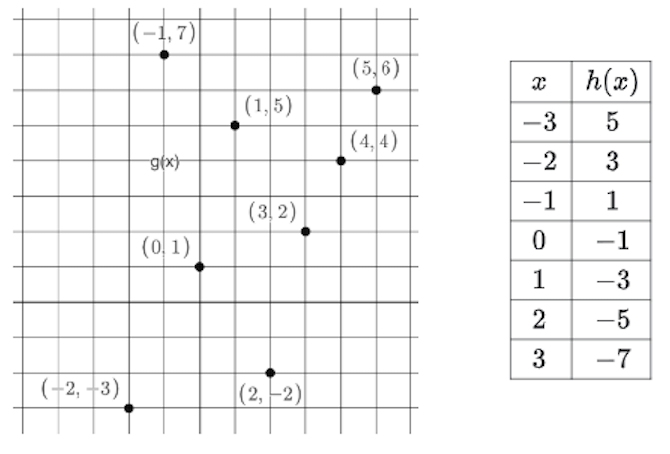
\includegraphics[width=5.0in]{warnberg-pre}

The picture in the upper left shows the graph of a function called $g(x)$ while the table on the right shows the inputs/outputs for a function called $h(x)$. Let $f(x) = x^2+6$

\begin{exm}
Find $(h \circ g)(3)$
\end{exm}
\vskip10pt
\begin{exm}
Find $(g+h)(2)$
\end{exm}
\vskip10pt
\begin{exm}
Find $(h \circ g \circ h)(-2)$
\end{exm}
\vskip10pt
\begin{exm}
Find $5 + g(5)$
\end{exm}
\vskip10pt
\begin{exm}
Find $10 + (f \circ h \circ g)(-2)$
\end{exm}
\vskip10pt

%\newpage
\renewcommand{\booksection}{One-to-one functions and Inverse Functions}
\renewcommand{\pageheader}{\booksection }
\section*{\LARGE \pageheader}
%\begin{concepts}
%\item 
%\item 
%\item 
%\item 
%\end{concepts}

%
%\begin{concepts}
% \item  Inverse functions
%	\item Horizontal line test
%\end{concepts}
%\vspace{1cm}



\section{1-1 Functions}
 A function $f(x)$ is called $1-1$ (one-to-one) if for every output, there is exactly 1 corresponding input. Said another way, if $a\neq b$, then $f(a)\neq f(b)$.   In other words, if $f(a)=f(b)$, then $a=b$.   
 It turns out that $1-1$ functions pass the \underline{Horizontal Line Test (HLT)}: every horizontal line passes through the graph at most 1 time. 


\section{Inverse Functions}
Given a $1-1$ function $f$, we define the \underline{inverse of $f$} to be the function $g$ so that 

$$g(b)=a ~~\mbox{exactly when}~~ f(a)=b. $$ The inverse of $f$ is denoted $f^{-1}$. 



\begin{center}
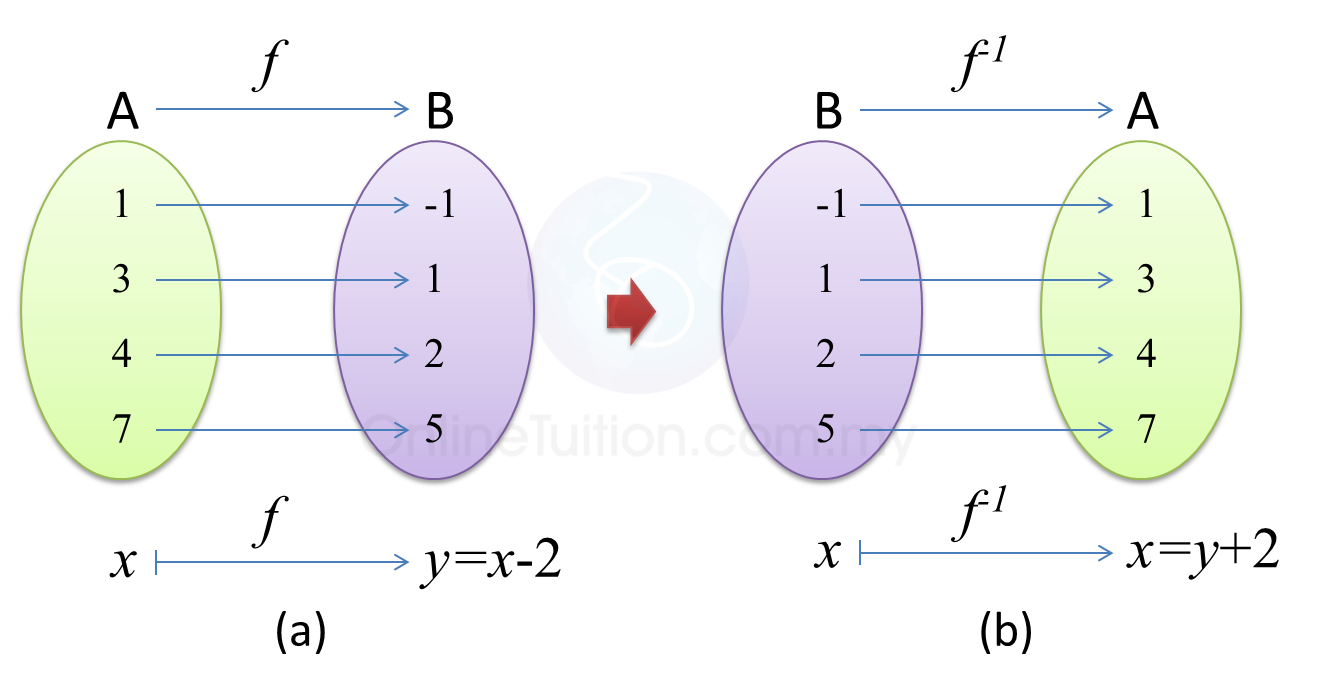
\includegraphics[scale=.4]{inversefunction.png}
\end{center}


%\newpage

\subsection{Properties of Inverses}
Here is a list of properties about inverse functions:
\begin{itemize}
	\item  The domain of $f$ is the range of $f^{-1}$.  
	\item  The range of $f$ is the domain of $f^{-1}$. 
		\item  $(f\circ f^{-1})(x)=x$ and $(f^{-1}\circ f)(x)=x$
		\item The graph of $f^{-1}$ is the graph of $f$ reflected across the line $y=x$  
		
		\begin{center}
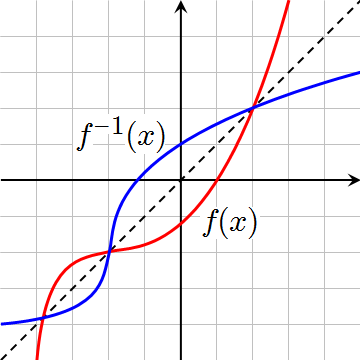
\includegraphics[scale=.25]{Inverse_Function_Graph.png}\vskip10pt
\end{center}
\end{itemize}

%\newpage
\everymath{\displaystyle}
\begin{exm}{Show that $f(x)=\frac{3}{x}$ is its own inverse.}
\end{exm}\vskip10pt

\begin{exm}{Explain why $f(x)=x^2$ and $g(x)=\sqrt{x}$ are {\it NOT} inverse functions.}
\end{exm}\vskip10pt

%\newpage
\everymath{\displaystyle}
\begin{exm}{Modify the domain of $f(x)=x^2$ so that $f(x)=x^2$ {\it IS} the inverse to $g(x)=\sqrt{x}$.}
\end{exm}\vskip10pt

\begin{exm}{If $f(2)=3, ~g^{-1}(3)=5$, and $f(5)=0$,\\ what is $(f^{-1}\circ g^{-1}\circ f)(2)$?}
\end{exm}\vskip10pt



%\newpage
\everymath{\displaystyle}
\begin{exm}{Show that $f(x)=3x+4$ and $f^{-1}(x)=\frac{x-4}{3}$ are indeed inverses by showing that $(f\circ f^{-1})(x)=x$ and $(f^{-1}\circ f)(x)=x$.}
\end{exm}\vskip10pt

\begin{exm}{Graph both  $f(x)=3x+4$ and $f^{-1}(x)=\frac{x-4}{3}$ to verify that they are reflections of each other across the line $y=x$.}
\end{exm}\vskip10pt

%\newpage

\begin{bmethod}{How to Find the Inverse Function}{}
Given a $1-1$ function $f(x)$
\begin{enumerate}
	\item  Change $f(x)$ to $y$.
	\item  Switch {\it ALL} $x$'s and $y$'s:  
		\item Solve for $y$: 
	\item  Change $y$ back to $f^{-1}(x)$ 
\end{enumerate}	
\end{bmethod}

\everymath{\displaystyle}
\begin{exm}{Find the inverse to $f(x)=\frac{2x-4}{3+x}$ and check your work.}
\end{exm}\vskip10pt

\begin{exm}{Find the inverse to $f(x)=\frac{x+3}{5x-6}$ and check your work.}
\end{exm}\vskip10pt



%\newpage
\everymath{\displaystyle}
\begin{exm}{Find the inverse to $f(x)=\sqrt[3]{x-2}+4$ and check your work.}
\end{exm}\vskip10pt

\begin{exm}{Given the graph of $f$ below, sketch the graph of $f^{-1}$.
				\begin{center}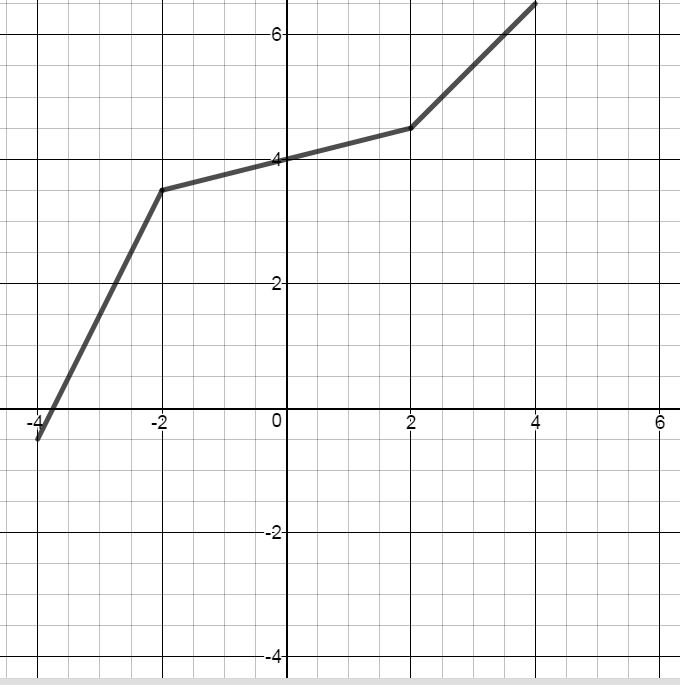
\includegraphics[scale=.3]{inverse.JPG}
\end{center}}
\end{exm}\vskip10pt


%\newpage

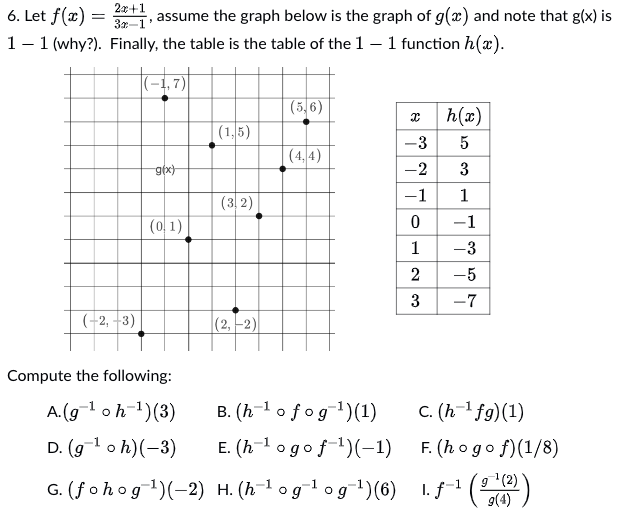
\includegraphics[width=5.5in]{warnberg-post}



%\newpage
\renewcommand{\booksection}{Exponential Functions}
\renewcommand{\pageheader}{\booksection }
\section*{\LARGE \pageheader}
%
%\begin{intro}
%\begin{abstract}
%$$e\approx 2.71828182846~~~~~~~~~~~~f(x)=a^x$$
%\end{abstract}
%\end{intro}
%
%
%\begin{concepts}
% \item  Exponential functions
%	\item The number $e$
%\end{concepts}
%\vspace{1cm}



\section{Exponential Functions}
 An \underline{exponential function} is of the form $f(x)=a^x$, for a constant $a>0$.    If $a>1$, the graph of $f(x)$ has the {\it general shape} given below: 
		\begin{center}
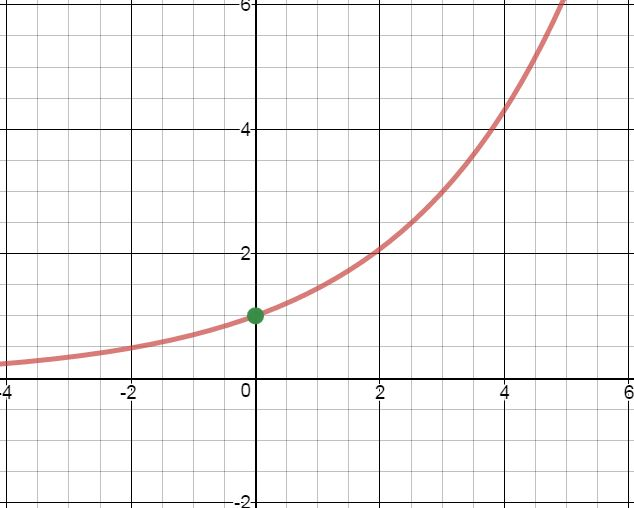
\includegraphics[scale=.25]{exp1.JPG}
\end{center}
If $0<a<1$, the graph of $f(x)$ has the {\it general shape} given below:   
		
		\begin{center}
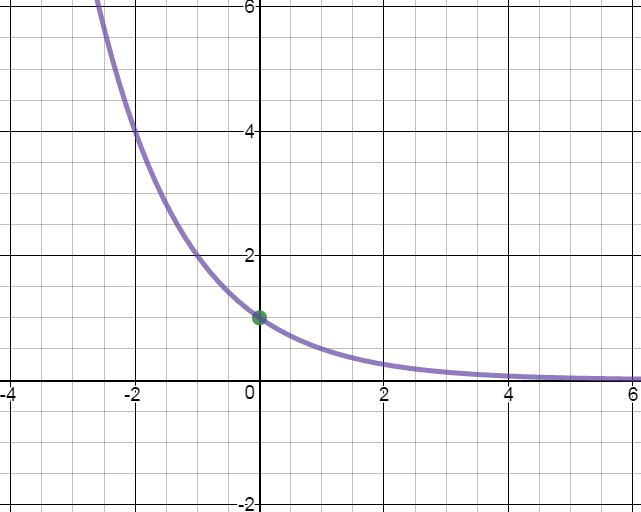
\includegraphics[scale=.25]{exp2.JPG}
\end{center}







\subsection{Properties of Exponential Functions}
   All exponential functions of the form $f(x)=a^x, a>0$ pass through the point $(0,1)$.  
	\begin{itemize}
	\item $f(0)=a^0=1\rightarrow (0,1)$ is on the graph of $f$   
\end{itemize}	
Here are some additional properties:
\begin{itemize}
		\item The domain of $f(x)=a^x$ is $(-\infty, \infty)$.  
			\item The range of $f(x)=a^x$ is $(0, \infty)$.   
				\item  $f(x)=a^x$ has a horizontal asymptote at $y=0$. 
	\item  $f(x)=a^x$ is a $1-1$ function and hence has an inverse. 
		\item   $a^x=a^y$ exactly when $x=y$.
\end{itemize}	




\subsection{The Number $e$}
The number $e$ is an irrational number between 2 and 3. In fact,
	$$e\approx 2.71828182846$$
Since $e$ is a number, it makes sense to talk about the exponential function $f(x)=e^x.$ 	

%\newpage
\everymath{\displaystyle}
\begin{exm}{Graph the function $f(x)=e^x$ and identify its domain and range.}
\end{exm}\vskip10pt

\begin{exm}{Graph the function $f(x)=2^{-x}$.}
\end{exm}\vskip10pt

%\newpage
\everymath{\displaystyle}
\begin{exm}{Graph the function $g(x)=3^{x+2}$. }
\end{exm}\vskip10pt

\begin{exm}{Graph the function $h(x)=-e^{x}-4$.}
\end{exm}\vskip10pt

%\newpage
\everymath{\displaystyle}
\begin{exm}{Graph the exponential function of the form $f(x)=Ba^{-x}+C$ that has a horizontal asymptote at $y=72$, $y$-intercept at 425, and passes through the point (1, 248.5).}
\end{exm}\vskip10pt

\begin{exm}{Solve $\left(\frac{1}{2}\right)^{6-x}=2$.}
\end{exm}\vskip10pt

%\newpage
\everymath{\displaystyle}
\begin{exm}{Solve $9^{2x}\cdot\left(\frac{1}{3}\right)^{x+2}=27\cdot(3^x)^{-2}$.}
\end{exm}\vskip10pt

\begin{exm}{Find the zeros to $f(x)=x^2(2e^{2x})+4x(e^{2x})+e^{2x}.$}
\end{exm}\vskip10pt



%\newpage

\begin{exm}
Given $A = 1000$ and $r=0.04$ and $t=5$, solve\footnote{This is a {\bf finance} problem, and the value of $P$ answers the following question: if an account earns $4\%$ interest compounded continuously, how much money should be deposited now so that the account balance is $\$1000$ in $5$ years?} for $P$ in $A=Pe^{rt}$. 
\end{exm}



%\newpage
\renewcommand{\booksection}{Logarithms}
\renewcommand{\pageheader}{\booksection }
\section*{\LARGE \pageheader}
%
%\begin{concepts}
% \item  Logarithmic functions
%	\item Log properties
%	\item Circle Trick
%\end{concepts}
%\vspace{1cm}



\section{Defining the Logarithmic Functions}

  Recall that $f(x)=a^x$ is a $1-1$ function and hence has an inverse.  In fact, we can even graph it:
\begin{center}
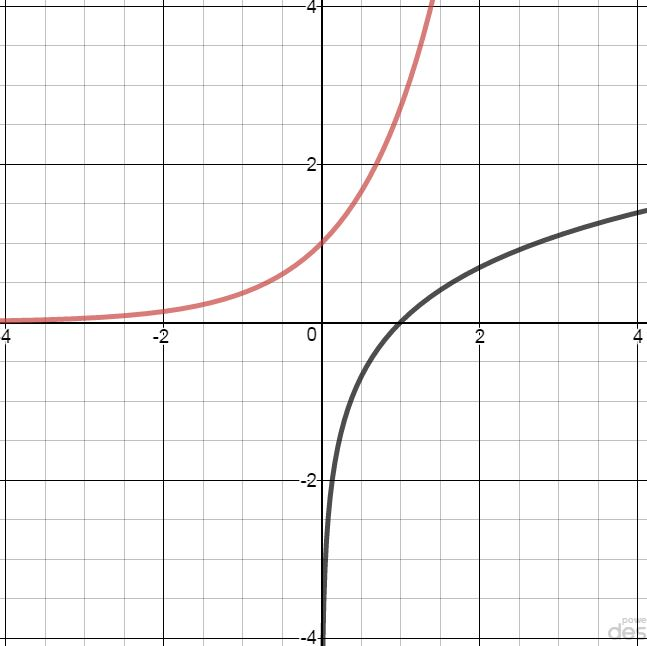
\includegraphics[scale=.4]{log2.JPG}
\end{center}

 If $f(x)=a^x$, then we know what $f^{-1}(x)$ {\it looks} like because it is reflected across the line $y=x$.  We also know that the domain of $f^{-1}(x)$ is $(0, \infty)$ and that the range of $f^{-1}(x)$ is $(-\infty, \infty)$. 
Even better, we can {\it evaluate} $f^{-1}(x)$: 
			\begin{itemize}
	\item   If $f(x)=2^x$, what is $f^{-1}\left(\frac{1}{4}\right)$?
	\item    $f^{-1}\left(\frac{1}{4}\right)=b$ exactly when $f(b)=\frac{1}{4}$ 
		\item $f(b)=\frac{1}{4}$ means $2^b=2^{-2}\rightarrow b=-2$ 
		\item  So, $f^{-1}\left(\frac{1}{4}\right)=-2$.  
\end{itemize}	

We can ask a very natural question: What is this function? it turns out that  given an exponential function $f(x)=a^x$, its inverse, $f^{-1}(x)$ is called the logarithm base $a$ and is denoted: $$f^{-1}(x)=\log_a(x).$$ 

\begin{blanguage}{Logarithm}{}
When seeing/writing $\log_a(x)$, say ``log base $a$ of $x$''.

Do not leave out the word \underline{base} and do no leave out the word \underline{of}. The \underline{of} is the same \underline{of} in Language Discussion~\ref{language:fofx} to remind you we have a function (even though the name of the function is more than just the letter $f$).
\end{blanguage}


\section{The Logarithmic Function}
 For each $a>0$, there is a different ``log base $a$'' function. And, there are two very special logarithms: 
	\begin{itemize}
	\item $\log_{10}(x)=\log(x)$ 
	\item   $\log_e(x)=\ln(x)$ 
 \end{itemize}
The domain for every log function is $(0, \infty)$. The range for every log function is $(-\infty, \infty)$. All log functions have the same shape and pass through $(1,0)$. This means $\log_a(1)=0$ for all $a>0$.  



\subsection{Circle Trick}
 For every logarithmic equation, there is a corresponding exponential equation.     This is useful because if you have an exponential equation you can't solve, convert it to a log equation. If you have a log equation you can't solve, convert it to an exponential equation.   
	Recall that $f(x)=y\Leftrightarrow f^{-1}(y)=x$. For our two functions, this means $$b^x=a\Leftrightarrow log_b(a)=x.$$

%\newpage

\begin{bmethod}{Circle Trick}{}		
		\begin{center}
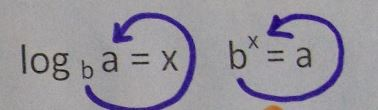
\includegraphics[scale=1]{circletrick.JPG}
\end{center}
\end{bmethod}

\everymath{\displaystyle}
\begin{exm}{Evaluate the following logarithms: $\log_9(3)$, $\log_2\left(\frac{1}{8}\right)$, $\log_4(-5)$.}
\end{exm}\vskip10pt

\begin{exm}
Given $A = 1000$ and $r=0.04$ and $P=850$, solve\footnote{This is a {\bf finance} problem, and the value of $t$ answers the following question: if an account earns $4\%$ interest compounded continuously, how many years will it take an account with starting balance $\$850$ to eventually have a balance of $\$1000$?} for $t$ in $A=Pe^{rt}$. 
\end{exm}
\vskip10pt

%\newpage
\begin{exm}{Solve $\log_2(x+9)=4$.}
\end{exm}\vskip10pt

\everymath{\displaystyle}
\begin{exm}{Sketch the graph of $\log_2|x|+2$.}
\end{exm}\vskip10pt


%\newpage
\subsection{Logarithmic Properties}
Below are a list of logarithmic properties

\begin{bformula}{}{}
$\log_a(x)=\log_a(y)$ exactly when $x=y$. 
\end{bformula}

\begin{bformula}{Laws of Logarithms}{}
\begin{itemize}
	\item   $\log_a(x^k)=k\log_a(x)$ 
		\item  $\log_a(xy)=\log_a(x)+\log_a(y)$
			\item $\log_a\left(\frac{x}{y}\right)=\log_a(x)-\log_a(y)$   
\end{itemize}	
\end{bformula}

\everymath{\displaystyle}
\begin{exm}{Use the log laws to expand the logarithms as much as possible: $$\ln\left(\frac{A^5B^3}{C^4D^2}\right)$$.}
\end{exm}\vskip10pt

\begin{exm}{Use the log laws to expand the logarithms as much as possible: $$\log\sqrt[3]{\frac{A}{B^2C^5}}$$.}
\end{exm}\vskip10pt

%\newpage
\everymath{\displaystyle}
\begin{exm}{Use the log laws to expand the logarithms as much as possible: $$\log\left(\frac{\sqrt{x+6}}{x^4e^{2x}}\right)$$.}
\end{exm}\vskip10pt

\begin{exm}{Use the log laws to expand the logarithms as much as possible: $$\ln\sqrt{\frac{x+9}{3x+1}}$$.}
\end{exm}\vskip10pt

%\newpage
\everymath{\displaystyle}
\begin{exm}{Use the log laws to expand the logarithms as much as possible: $$\log\left( \frac{x^2}{\sqrt[3]{x-2}(2x+3)^5} \right)$$.}
\end{exm}\vskip10pt

\begin{exm}{Rewrite $\log_3(x) + \log_3(y) - 7\log_3(z)$ as one logarithm.}
\end{exm}\vskip10pt

%\newpage
\everymath{\displaystyle}
\begin{exm}{Rewrite $\ln(x) + \ln(y) - 7\ln(z)$ as one \emph{natural} logarithm.}
\end{exm}\vskip10pt

%\newpage

\begin{bmethod}{}{}
If $\log_a(x)=\log_a(y)$ then $x=y$. 
\end{bmethod}

\begin{bhabit}{}{}
If the original equation had variables in an input to any logarithm, check to ensure there are no false solutions. (Any solution which causes us to take the logarithm of $0$ or negative is a false solution. This is because the input to any logarithm must be positive.)
\end{bhabit}

\begin{exm}{Solve $\ln(x+6)-\ln(10)=\ln(x-1)-\ln(2)$ for $x$.}
\end{exm}\vskip10pt

%\newpage

\begin{exm}{Solve $\log(x+4)=2-\log(x-2)$.}
\end{exm}\vskip10pt


%\newpage

\begin{bformula}{Logs and Exps are inverses}{}
\begin{itemize}
				\item  $\log_a(a^x)=x$ 
	\item   $a^{\log_a(x)}=x$  
\end{itemize}	
\end{bformula}

\begin{exm}
Simplify $2^{10 \log_2(m)}$
\end{exm}
\vskip40pt

\begin{exm}
Simplify $\log_3(9^x)$
\end{exm}
\vskip40pt


\begin{bformula}{}{}
$\log_a(1)=0$ 
\end{bformula}

%\newpage

\begin{bformula}{Change of base}{}
$\log_a(x)=\frac{\ln(x)}{\ln(a)}$ 
\end{bformula}

\begin{exm}
Solve\footnote{This is a {\bf finance} problem. For a house loan of $\$215000$ with interest compounding at a rate of $6\%$ monthly, and monthly payments of $\$1100$, finding $t$ tells you how many years a family would have this mortgage.} for $t$ in
\[ V = P \cdot \frac{1 - (1 + \frac{r}{m})^{-mt}}{\frac{r}{m}} \]
given $V=215000$ and $r=0.06$ and $m=12$ and $P=1100$. State an exact answer, and then write what should be input into a calculator which only understands natural logarithms.
\end{exm}

\vskip10pt

\begin{exm}
Write\footnote{This expression came from a chemistry problem.} how should 
$$-\log_2(3.9 \times 10^{-4}) + \log_5 \dfrac{0.038}{0.183}$$
be input into a calculator
\end{exm}

%
%\subsection{Proofs}
%All of the log properties can be proven with the assumption that the log function is the inverse to an exponential function. We will show two proofs here. First, we will prove that $\log_a(xy)=\log_a(x)+\log_a(y)$.
%\begin{align*}
%   xy&=xy\\ 
%  \Leftrightarrow a^{\log_a(xy)}&=\left(a^{\log_a(x)}\right)\left(a^{\log_a(y)}\right) \\
%   \Leftrightarrow a^{\log_a(xy)}&=a^{\log_a(x)+\log_a(y)}\\
%   \Leftrightarrow \log_a(xy)&=\log_a(x)+\log_a(y)\\
%\end{align*} 
%
%Next, we will prove that $\log_a(x)=\frac{\ln(x)}{\ln(a)}$
%\begin{align*}
%   x&=x\\ 
%   \Leftrightarrow  a^{\log_a(x)}&=x\\
%   \Leftrightarrow \left(e^{\ln(a)}\right)^{\log_a(x)}&=e^{\ln(x)}\\
%   \Leftrightarrow e^{\ln(a)\log_a(x)}&=e^{\ln(x)}\\
%   \Leftrightarrow \ln(a)\log_a(x)&=\ln(x)\\
%   \Leftrightarrow \log_a(x)&=\frac{\ln(x)}{\ln(a)}\\
%\end{align*} 







%\newpage
\everymath{\displaystyle}

\begin{exm}{Let $f(x)=\ln(x-2)$. Use transformations to sketch the graph of $f$.
    Then find the domain and vertical asymptote. Let $g(x)=\ln(x^2+2x-15)$ 
    Use algebra (including a sign chart) to find the domain and vertical asymptotes.
    Then use desmos to sketch the graph of $g$ and check your work}
\end{exm}\vskip10pt








%\newpage
\renewcommand{\booksection}{Exponential and Logarithmic Equations}
\renewcommand{\pageheader}{\booksection }
\section*{\LARGE \pageheader}
%
%\begin{concepts}
% \item  Solving equations with exponents and logarithms
%\end{concepts}
%\vspace{1cm}

\everymath{\displaystyle}
\begin{exm}{Solve for $x$ in the equation  \quad
$7^{2x+3} = 3^{x-2}$.}
\end{exm}\vskip10pt

\begin{exm}{Solve for $x$ in the equation  \quad
$\log \sqrt{x-9} = 2$.}
\end{exm}\vskip10pt

%\newpage
\everymath{\displaystyle}
\begin{exm}{Solve for $x$ in the equation \quad\\
$\log_6(x-4) - \log_6(3x-10) = \log_6(\frac1x)$.}
\end{exm}\vskip10pt

\begin{exm}{Solve for $x$ in the equation \quad
$3 \log_5 (x) = 2 \log_5(4)$.}
\end{exm}\vskip10pt

%\newpage
\everymath{\displaystyle}
\begin{exm}{Solve for $x$ in the equation\\
$\log (5x+1) = \log(100) + \log(2x -3)$}
\end{exm}\vskip10pt

\begin{exm}{Solve for $x$ in the equation  \quad
$\log(x^3) = (\log x)^3$.}
\end{exm}\vskip10pt

%\newpage
\everymath{\displaystyle}
\begin{exm}{Solve $ 6e^{2x}=1800$. }
\end{exm}\vskip10pt

\begin{exm}{Solve $ 2^t=5^{7-4t}$.}
\end{exm}\vskip10pt

%\newpage
\everymath{\displaystyle}
\begin{exm}{Solve $ e^{2z}+3e^z-40=0$.}
\end{exm}\vskip10pt

\begin{exm}{Solve $ \frac{2^x-2^{-x}}{4}=3$.}
\end{exm}\vskip10pt


%\newpage

\begin{bformula}{Exponential Growth/Decay}{}
$$n(t)=n_oe^{rt},$$ where $n(t)$ is the population at time $t$, $n_o$ is the initial size of population, $r$ is the relative rate of growth, $t$ is time.
\end{bformula}

\begin{bformula}{Newton's Law of Cooling}{}
$$T(t)=T_s+D_oe^{-kt},$$ where $D_o$ is the initial temperature difference between object and surroundings, $T_s$ is the temperature of the surroundings, $t$ is time, and $k$ is the constant dependent on object. 
\end{bformula}


\everymath{\displaystyle}
\begin{exm}{A species of bird was introduced to a certain island 25 years ago. Biologists observe that the population doubles every 10 years and now the population is 13,000. What was the initial population? What will the population be in 5 years? Graph the function that models this growth.}
\end{exm}\vskip10pt






%\newpage
\everymath{\displaystyle}
\begin{exm}{}{A certain bacteria culture has a relative growth rate of 12\% per hour but in the presence of an antibiotic, the relative growth rate is reduced to 5\% per hour. The initial number of bacteria in the culture is 22. Find the projected population after 24 hours if (a) no antibiotic is present, (b) antibiotics are present.}
\end{exm}\vskip10pt

\begin{exm}{}{The half-life of cesium-17 is 30 years. Suppose we have a 10-g sample. How much of the sample will be left in 80 years? How long will it take for the sample to decrease to 2-g?}
\end{exm}\vskip10pt




%\newpage
\everymath{\displaystyle}
\begin{exm}{}{Newton's Law of Cooling is used in homicide investigations to determine the time of death. The normal body temperature is 98.6 F. Immediately following death, the body begins to cool. It has been determined experimentally that the constant in Newton's Law of Cooling is approximately $k=0.1947$, assuming time is measured in hours. Find a function that models the temperature $t$ hours after death. Suppose the surrounding environment is 60 F. If the temperature of the body is now 72 F, how long ago was death? }
\end{exm}\vskip10pt



%\newpage
\renewcommand{\booksection}{Appendix A: Completing the Square}
\renewcommand{\pageheader}{\booksection }
\section*{\LARGE \pageheader}

{\bf Complete the square to solve a typical quadratic equation}\label{cts-example}
\begin{center}
\[3x^2+5x+7=6\]
Subtract $7$ on both sides.
\[3x^2+5x=-1\]
Divide by $3$ on both sides. Be sure to divide the \emph{entire} left side by $3$.
\[\frac{3x^2+5x}{3}=\frac{-1}{3}\]
As written, the two $3$'s on the left side above don't cancel because the $3$ in the numerator is not a factor. Rewrite.
\[\frac{3x^2}{3}+\frac{5x}{3}=\frac{-1}{3}\]
The rewrite above used the formula $\frac{r}{t}+\frac{s}{t}=\frac{r+s}{t}$. Now use $\frac{mp}{np}=\frac{m}{n}$ to cancel $3$'s.
\[x^2+\frac{5x}{3}=\frac{-1}{3}\]
Because $\frac{5x}{3}=\frac{5}{3}\cdot\frac{x}{1}=\frac{5}{3}x$ using the formula $\frac{q}{r}\frac{s}{t}=\frac{qs}{rt}$, replace $\frac{5x}{3}$ with $\frac{5}{3}x$.
\[x^2+\frac{5}{3}x=\frac{-1}{3}\]
With coefficient $\frac{5}{3}$, the length of second stick is $\frac{5}{2 \cdot 3}$. By squaring, $(\frac{5}{2 \cdot 3})^2=\frac{5^2}{(2 \cdot 3)^2}=\frac{5^2}{4 \cdot 3^2}=\frac{25}{36}$. Add $\frac{25}{36}$ to both sides.
\[x^2+\frac{5}{3}x+\frac{25}{36}=\frac{25}{36}-\frac{1}{3}\]
Factor left side. On right side, take the fraction after the minus sign and multiply by $12$ on top and bottom.
\[\left(x+\frac{5}{6}\right)^2=\frac{25}{36}-\frac{12}{36}\]
Simplify the right side by using the fraction subtraction formula $\frac{m}{p}-\frac{n}{p}=\frac{m-n}{p}$.
\[\left(x+\frac{5}{6}\right)^2=\frac{13}{36}\]
Square root both sides, and put $\pm$ on one side. %Putting $\pm$ on left side would necessitate a set of parentheses, so put $\pm$ on right side.
\[\sqrt{\left(x+\frac{5}{6}\right)^2}=\pm \sqrt{\frac{13}{36}}\]
Square root and square undo each other on the left side.
\[x+\frac{5}{6}=\pm\sqrt{\frac{13}{36}}\]
Use $\sqrt[n]{\frac{c}{d}}=\frac{\sqrt[n]{c}}{\sqrt[n]{d}}$ to rewrite everything past the $\pm$ on the right side.
\[x+\frac{5}{6}=\pm\frac{\sqrt{13}}{\sqrt{36}}\]
Simplify square root in denominator. Note that $\sqrt{36}$ is $6$ because $(6)^2=36$.
\[x+\frac{5}{6}=\pm\frac{\sqrt{13}}{6}\]
Subtract $\frac{5}{6}$ on both sides.
\[x=-\frac{5}{6}\pm\frac{\sqrt{13}}{6}\]
Use the fraction addition/subtraction rule $\frac{m}{p} \pm \frac{n}{p}=\frac{m \pm n}{p}$.
\[x=\frac{-5 \pm \sqrt{13}}{6}\]
\end{center}

%\newpage

{\bf Complete the square to get the Quadratic Formula} \label{derive-qf}
This is the same type of work done in the specific example shown starting on page \pageref{cts-example}
\begin{center}
\[ax^2+bx+c=0\]
Subtract $c$ on both sides.
\[ax^2+bx=-c\]
Divide by $a$ on both sides. Be sure to divide the \emph{entire} left side by $a$.
\[\frac{ax^2+bx}{a}=\frac{-c}{a}\]
As written, the two $a$'s on the left side above don't cancel because the $a$ in the numerator is not a factor. Rewrite.
\[\frac{ax^2}{a}+\frac{bx}{a}=\frac{-c}{a}\]
The rewrite above used the formula $\dfrac{r}{t}+\dfrac{s}{t}=\dfrac{r+s}{t}$.\\ Now use $\dfrac{mp}{np}=\dfrac{m}{n}$ to cancel $a$'s.
\[x^2+\frac{bx}{a}=\frac{-c}{a}\]
Because $\frac{bx}{a}=\frac{b}{a}\cdot\frac{x}{1}=\frac{b}{a}x$ using the formula $\frac{q}{r}\frac{s}{t}=\frac{qs}{rt}$, replace $\frac{bx}{a}$ with $\frac{b}{a}x$.
\[x^2+\frac{b}{a}x=\frac{-c}{a}\]
\fbox{
\begin{minipage}[ht]{6.5in}
\vskip4pt
\begin{itemize}
\item The linear coefficient is $\dfrac{b}{a}$, not $\dfrac{b}{a}x$. Do not include the $x$.
\item Since the linear coefficient is $\dfrac{b}{a}$, the length of the second stick is $\dfrac{b}{a} \div 2 = \dfrac{b}{a} \div \dfrac21 = \dfrac{b}{a} \cdot \dfrac12 = \dfrac{b}{2a}$
\item Since the second stick is $\dfrac{b}{2a}$, the constant to add to both sides is $\left(\dfrac{b}{2a}\right)^2 = \dfrac{b^2}{(2a)^2} = \dfrac{b^2}{2^2a^2} = \dfrac{b^2}{4a^2}$
\end{itemize}

\begin{center}
\begin{tikzpicture}
\node at (2,-1.6) {\underline{Picture of} $x^2+\dfrac{b}{a}x$};
\draw (0,0) -- (3,0) -- (3,3) -- (0,3) -- cycle;
\draw (3,0) -- (4,0) -- (4,3) -- (3,3);
\draw (0,0) -- (0,-1) -- (3,-1) -- (3,0);
%
\node at (-.3,1.5) {$x$};
\node at (-.3,-.5) {$\frac{b}{2a}$};
\node at (1.5,3.3) {$x$};
\node at (3.5,3.6) {$\frac{b}{2a}$};
%
\node at (1.5,1.5) {$x^2$};
\node at (3.5,1.5) {$\frac{b}{2a}x$};
\node at (1.5,-.5) {$\frac{b}{2a}x$};
\end{tikzpicture}
\hskip60pt
\begin{tikzpicture}
\node at (2,-1.6) {\underline{Picture of} $x^2+\dfrac{b}{a}x+\dfrac{b^2}{4a^2}$};
\draw (0,0) -- (3,0) -- (3,3) -- (0,3) -- cycle;
\draw (3,0) -- (4,0) -- (4,3) -- (3,3);
\draw (0,0) -- (0,-1) -- (3,-1) -- (3,0);
\draw (3,-1) -- (4,-1) -- (4,0); % new
%
\node at (-.3,1.5) {$x$};
\node at (-.3,-.5) {$\frac{b}{2a}$};
\node at (1.5,3.3) {$x$};
\node at (3.5,3.6) {$\frac{b}{2a}$};
%
\node at (1.5,1.5) {$x^2$};
\node at (3.5,1.5) {$\frac{b}{2a}x$};
\node at (1.5,-.5) {$\frac{b}{2a}x$};
\node at (3.5,-.5) {$\frac{b^2}{4a^2}$}; % new
\end{tikzpicture}
\end{center}
\end{minipage}}



\[x^2+\frac{b}{a}x+\frac{b^2}{4a^2}=\frac{b^2}{4a^2}-\frac{c}{a}\]
Factor left side. On right side, take the fraction after the minus sign and multiply by $4a$ on top and bottom.
\[\left(x+\frac{b}{2a}\right)^2=\frac{b^2}{4a^2}-\frac{4ac}{4a^2}\]
Simplify the right side by using the fraction subtraction formula $\frac{m}{p}-\frac{n}{p}=\frac{m-n}{p}$.
\[\left(x+\frac{b}{2a}\right)^2=\frac{b^2-4ac}{4a^2}\]
Square root both sides, and put $\pm$ sign on one side.% Putting $\pm$ on left side would necessitate a set of parentheses, so put $\pm$ on right side.
\[\sqrt{\left(x+\frac{b}{2a}\right)^2}=\pm \sqrt{\frac{b^2-4ac}{4a^2}}\]
Square root and square undo each other on the left side.
\[x+\frac{b}{2a}=\pm\sqrt{\frac{b^2-4ac}{4a^2}}\]
Use $\sqrt[n]{\frac{c}{d}}=\frac{\sqrt[n]{c}}{\sqrt[n]{d}}$ to rewrite everything past the $\pm$ on the right side.
\[x+\frac{b}{2a}=\pm\frac{\sqrt{b^2-4ac}}{\sqrt{4a^2}}\]
Simplify square root in denominator. Note that $\sqrt{4a^2}$ is $2a$ because $(2a)^2=4a^2$.
\[x+\frac{b}{2a}=\pm\frac{\sqrt{b^2-4ac}}{2a}\]
Subtract $\frac{b}{2a}$ on both sides.
\[x=-\frac{b}{2a}\pm\frac{\sqrt{b^2-4ac}}{2a}\]
Use the fraction addition/subtraction rule $\frac{m}{p} \pm \frac{n}{p}=\frac{m \pm n}{p}$.
\[x=\frac{-b \pm \sqrt{b^2-4ac}}{2a}\]
\end{center}








%
%
%%\newpage
%
%\begin{exm}
%\end{exm}
%\begin{exm}
%\end{exm}
%
%
%
%
%%\newpage
%
%\section{BORROW}
%
%\begin{bhabit}{}{part-of-speech}
%Every time you encounter a new definition, determine if the thing being defined is a noun, an adjective, a verb, etc.
%\end{bhabit}
%
%\begin{bwarning}{Do not ignore language issues and grammar}{do-not-ignore}
%Be sure to write definitions in complete sentences. Think of whether a word being defined is a noun, adjective, verb, etc. and clearly convey this when you write definitions. Adjectives should only be applied to \emph{appropriate} nouns. Do not ignore this advice regarding \end{bwarning}
%
%\begin{bhabit}{What types of objects are elements of a set?}{set-of-what}
%Every time you encounter a set, ask yourself what kind of object are elements of the set.
%\end{bhabit}
%The habit just mentioned is a clue into the following important fact: the elements of a set are not necessarily numbers. For example, $\mathbb{H}$ is a set, even though there are no numbers in this set.
%
%
%
%\begin{bmethod}{Proving $x \in S$ if $S$ is in build running through set format}{proving-element-in-set-running}
%If $S = \{f(c) : c \in R \}$, first rewrite $S$ as $S = \{z : \exists c \in R \text{ s.t. } z=f(c)\}$. To prove $x \in S$,
%Sameple text
%\end{bmethod}
%
%
%
%
%\begin{bformula}{Distributive Law}{stuf}
%$a(b+c)=ab+ac$
%\end{bformula}
%
%
%
%
%
%\begin{exercise}
%Let $T$ be the set of all $2 \times 2$ matrices (with real entries). Let us define the function $\phi : T \to \mathbb{R}$ by the rule $\phi(A)= \sqrt{2}\,\det(A)$. Prove $\phi : T \to \mathbb{R}$ is surjective, but not bijective.
%\end{exercise}

%%%%%%%%%%%%%%%%%%%%%%%%%%%%%%%%%%%%%%%%

%\printindex

\end{document}

SKIPPED
(3+x)/(x^2-9) <= 3
Graphing rational functions
rationalize denom
(2+i)/(3-i)

MAYBE
polynomial inqualities (graph polynomial functions?)


